% Version of Document Management
% $Revision: $

% Version which does not generate Table of Contents, to create a html then a chm version

\title{CodeBlocks User Manual}
\def\newcharencode{utf8}        % set character encoding
\ProvidesFile{booleans.tex}[2006/11/01 HighTec template]
\RequirePackage{snapshot}       % list dependencies in .dep
\RequirePackage{ifthen}         % control structures
\makeatletter
\@ifundefined{newcharencode}{   % cp1252
    \RequirePackage[ansinew]{inputenc}% package for input encoding under windows
}{
    %\RequirePackage{ucs}       % utf-8
    \RequirePackage[utf8]{inputenc}
}
\newboolean{html}               % specials for presentation with beamer.cls
\newboolean{book}               % print document as book
\newboolean{mathmode}           % specials for propser presentation
\newboolean{tabreg}             % for generation of list of tables otherwise set Tabreg false
\newboolean{figreg}             % for generation of list of figures otherwise set Figreg false
\newboolean{glossreg}           % for generation of glossary
\newboolean{acroreg}            % for generation of acronyms
\newboolean{nomreg}             % for generation of nomenclature
\newboolean{urlreg}             % for generation of url catalogue
\newboolean{bibreg}             % for generation of Bibliography otherwise set Bibreg false
\newboolean{multiidx}           % for generation of multiple index
\newboolean{changereg}          % list of changes
\newboolean{indreg}             % for generation of Index otherwise set Indreg false
\newboolean{shortdocu}          % use for short docu
%% set defaults %%%%%%%%%%%%%%%%%%%%%%%%%%%%%%%%%%%
\setboolean{html}{false}        % for option for common_pack.tex
\setboolean{book}{false}        % print document as book
\setboolean{mathmode}{false}    % enable amslatex
\setboolean{tabreg}{false}      % for generation of list of tables otherwise set Tabreg false
\setboolean{figreg}{false}      % for generation of list of figures otherwise set Figreg false
\setboolean{glossreg}{false}    % for generation of glossary
\setboolean{acroreg}{false}     % for generation of acronyms
\setboolean{nomreg}{false}      % for generation of nomenclature
\setboolean{urlreg}{false}      % for generation of url catalogue
\setboolean{bibreg}{false}      % for generation of Bibliography otherwise set Bibreg false
\setboolean{multiidx}{false}    % for generation of multiple index
\setboolean{changereg}{false}   % list of changes
\setboolean{indreg}{false}      % for generation of Index otherwise set Indreg false
\setboolean{shortdocu}{false}   % use for short docu
       % boolean declaration
% booleans already defined and set in mystyles/booleans, eventually set to an other value here ...
\setboolean{urlreg}{true}       % for url catalogue
\setboolean{bibreg}{false}      % for bibliography
\setboolean{indreg}{false}      % for index generation
\setboolean{shortdocu}{true}    % oneside document
%\setboolean{figreg}{true}       % for figure list
%\setboolean{tabreg}{true}       % for table list
\setboolean{html}{true}

%\def\lngfr{french}
%\def\lngen{english}
%\def\lngge{german}

%%%%% options %%%%%%%%%
\def\lang{english}
\def\graphmode{final}           % graphmodes: draft: box; final: including figures

% generate url catalog for toolchain
\def\urlfilename{mystyles/url_codeblocks}

%%%%%%%% parameter for titlepage %%%%%%%%%%
\def\Subject{Code::Blocks}
\def\Title{User Manual}
\def\DocVersion{2.1.11}

% style for documentation
\ProvidesFile{format_docu.tex}[2007/05/26 HighTec template]
%%%%%%%%%%%%%%%%%%%%%%%%%%%%%%%%%%%%%%%%%%%%%%%%%%%%%%%%%%%%%%%%%%%%%%%%%%%%%%%%%%%%%%%%%%%%%%%%%%%%%%%%%%%%%%%%%%%%%%%%%%%%%%%
% Some of the ifthenelse (but apparently/strangely not All) have problems when they are used by MikTeX 22.10 though it was OK 
% with a previous version 22.03, particularly when they are used to build an html version by htlatex.
% They have been replaced by the standard TeX syntax \if ...[ \else ... ]\fi in different .tex files within mystyles folder.
%%%%%%%%%%%%%%%%%%%%%%%%%%%%%%%%%%%%%%%%%%%%%%%%%%%%%%%%%%%%%%%%%%%%%%%%%%%%%%%%%%%%%%%%%%%%%%%%%%%%%%%%%%%%%%%%%%%%%%%%%%%%%%%
\ifthenelse{\boolean{shortdocu}}{\def\docupagemode{oneside}}{\def\docupagemode{twoside}}
%\ifthenelse{\boolean{shortdocu}}{\def\docupagemode{twoside=false}}{\def\docupagemode{twoside=true}}
\ifthenelse{\equal{\lang}{german}}{%
    % german language
    \documentclass[index=totoc,ngerman,12pt,\docupagemode,paper=a4,headings=normal,headsepline,numbers=noenddot,footsepline,\graphmode]{scrbook}
%    \documentclass[idxtotoc,ngerman,12pt,\docupagemode,a4paper,normalheadings,headsepline,pointlessnumbers,footsepline,\graphmode]{scrbook}
}{
    \ifthenelse{\equal{\lang}{french}}{%
    % french language
        \documentclass[index=totoc,french,12pt,\docupagemode,paper=a4,headings=normal,headsepline,numbers=noenddot,footsepline,\graphmode]{scrbook}
    }{
    % english by default
        \documentclass[index=totoc,english,12pt,\docupagemode,paper=a4,headings=normal,headsepline,numbers=noenddot,footsepline,\graphmode]{scrbook}
    }
}

\ifthenelse{\boolean{nomreg}}{\usepackage[\lang]{nomencl}\makeglossary}{}
\ifthenelse{\boolean{glossreg}}{\usepackage{glosstex}}{}

% common packages
\ProvidesFile{common_pack.tex}[2005/01/02 HighTec template]
\makeatletter
\@ifundefined{htmlmode}{\usepackage{mparhack}}{}% correct marginal in document
\makeatother
% select conditional text within document
\usepackage{version}
\def\includecomment{\includeversion}
\def\excludecomment{\excludeversion}

\ifthenelse{\equal{\lang}{german}}{%
    \usepackage[ngerman]{babel}                 % translate figure -> Abbildung etc.
    \usepackage{ngerman}                        % new sgerman hyphenation
}{}

%\ifthenelse{\equal{\lang}{french}}{%
%    \usepackage[french]{babel}                 % Should be nice, but give errors ! At least with listings package
%    \usepackage{french}
%}{}
% produce several index
\ifthenelse{\boolean{indreg}}%
{%
    \ifthenelse{\boolean{multiidx}}{\usepackage[makeindex]{splitidx}}{\usepackage[makeindex]{splitidx}}
    \newindex[Index]{idx}                       % common index
}{}
\usepackage{fancyvrb, listings}                 % verbatim input and complex verbatim
\usepackage{url}                                % breaking urls
\usepackage{float, morefloats}                  % utility for placing figures with here [H] option; subfigure placing% normally # of floats 18 -> with more float 38
\usepackage{afterpage}                          % figures not before first reference
\afterpage{\clearpage}                          %
\ifthenelse{\boolean{mathmode}}{\usepackage{amsbsy,amsmath,amstext,amsfonts,amssymb}}{}% for AMS-Latex -> formula
\usepackage{xcolor}                             % switch from color to xcolor package (driver independent)
\usepackage{ifpdf}                              % with this package \ifpdf \else \fi
\ifpdf                                          % We are not running pdftex
    \usepackage[pdftex, \graphmode]{graphicx}   % Package for graphics import
    \usepackage{epstopdf}                       % pdflatex understands eps -> use --shell-escape option for Texlive and --enable-write18 for Miktex
\else
    \usepackage[dvips, \graphmode]{graphicx}    % Package for graphic import of EPS, TIF, BMP
\fi
\usepackage{array,longtable,tabularx}           %%%%%%%%%% tool for tables; colortbl not used here
\def\tpath{tables/}                             % path for tables
\usepackage{xspace}                             % adds spaces in context without .! etc
\usepackage[\lang]{hyperref}                    % include hyperrefs in pdf; select lang for autoref
\usepackage{attachfile}                         % attach files in a pdf-document
%\ifpdf
    \graphicspath{{figures/svg/}{figures/png}{figures/pdf/}{figures/eps/}{../figures/svg/}{../figures/png}{../figures/pdf/}{../figures/eps/}}
%\else
%    \graphicspath{{figures/svg/}{figures/png/}{figures/pdf/}{figures/eps/}{../figures/svg/}{../figures/png/}{../figures/pdf/}{../figures/eps/}}
%\fi

\usepackage{makecell}
\usepackage{xcolor}
\usepackage{scrhack}    % Suggested in logs but not really useful apparently
\usepackage{enumitem}   % to be able to use [noitemsep] in enumerate, itemize,... to reduce the vertical step between \item

\topmargin=-1cm \oddsidemargin=0mm \evensidemargin=0mm
\textheight24cm \textwidth16cm \marginparsep=3mm \marginparwidth=15mm %\reversemarginpar
\partopsep 0pt %\topsep 0pt
\parskip 1.7ex plus0.3ex minus0.2ex \parindent 0pt
\frenchspacing \footskip 10mm \abovecaptionskip10pt

% setup for pdf generation
\ProvidesFile{hypersetup.tex}[2006/11/01 HighTec template]

\definecolor{dgreen}{rgb}{0,0.5,0.25}       % define colors
\definecolor{gray}{rgb}{0.5,0.5,0.5}
\definecolor{light}{rgb}{0.95,0.988,1}
\definecolor{webgreen}{rgb}{0, 0.5, 0}
\definecolor{webblue}{rgb}{0, 0, 0.5}
\definecolor{webred}{rgb}{0.5, 0, 0}
\definecolor{bluelight}{rgb}{.6, 0.8, 1}    % dark blue of hightec
\definecolor{bibblue}{rgb}{.1333, 0, 0.871} % dark blue of hightec

\def\Author{Code::Blocks Community}

\makeatletter
\@ifundefined{mykeywords}{\def\mykeywords{ }}{}
\makeatother

{\hypersetup{
%    ps2pdf,
%    bookmarks=true,
%    backref=true,
%    pagebackref=true,
    plainpages=false,
    extension=pdf,
    bookmarksopen=true,
    bookmarksnumbered=true,
    bookmarksopenlevel=0,
    breaklinks=true,
    colorlinks=true,
    linkcolor=webblue,
    citecolor=bibblue,
    filecolor=dgreen,
    extension=pdf,
    urlcolor=blue,
    pdffitwindow=true,
    pdfpagemode=UseOutlines,
    pdfpagelayout=SinglePage, % SinglePage
    pdfstartview=Fit,         % Fit, FitB
    pdfmenubar=true,
    pdftoolbar=true,
    pdfauthor = {\Author},
    pdftitle = {\Title},
    pdfsubject = {\Subject},
    baseurl = {},
    pdfcreator = {PdfLaTeX and hyperref package},
    pdfproducer = {pdflatex},
    pdfkeywords = {\mykeywords}
}

\attachfilesetup{
    color = {0 .5 0},
    mimetype = text/plain,
    subject = {Source Code},
    author = {\Author},
    description = {Example}
}
\def\attach#1{\textattachfile{#1}{#1}}

\ProvidesFile{macros.tex}[2006/02/01 HighTec template]
%%%%%%%%%%%%%%%% url catalog from addison wesley %%%%%%%%%%%%%%%%%%%%%%%%%%%%%
\makeatletter
\@ifundefined{htmlmode}{}{%
    \setboolean{html}{true}
}

\def\@URN#1{{\fontsize{8}{10}\selectfont#1}}
%\def\ShowURN#1{\@URN{#1}:\quad}
\def\ShowURN#1{\quad}
\newcommand{\urlbibitem}[2]{\bibitem#1#2}

\newenvironment{theurlbibliography}[1]
    {\chapter{URL catalog}
%  \label{URLBIB}\addcontentsline{toc}%
%       {chapter}{\protect\numberline{}{URL catalog}}
%  \markboth{URL catalog}{URL catalog}
    \begin{list}
        {\urlbiblabel{\arabic{enumiv}}}
        {
            \labelwidth\z@ \labelsep\z@ \leftmargin\parindent
            \itemindent-\parindent
            \usecounter{enumiv}%
            \let\p@enumiv\@empty
            \renewcommand\theenumiv{\@arabic\c@enumiv}}%
        \sloppy\clubpenalty4000\widowpenalty10000%
        \nonfrenchspacing
        \raggedright
        \addtolength\itemsep{0pt plus 2pt minus 2pt}%
        \small
    }
    {\renewcommand\@noitemerr
        {\@warning{Empty~ `theurlbibliography'~ environment}}
    \end{list}}

%%%%%%%%%%%%%%% macros %%%%%%%%%%%%%%%%%%%%%%%%%%%%%%%%%%
\ifthenelse{\equal{\lang}{german}}{%
    \def\hintname{Hinweis}
    \def\au{\glqq}%
    \def\ao{\grqq}%
    \def\gl{Gleichung~}%
    \def\pa{Seite~}%
    \ifthenelse{\boolean{html}}{%
        \newcommand{\pxref}[1]{\autoref{#1}}                        % for references
    }{%
        \newcommand{\pxref}[1]{\autoref{#1} auf \pa\pageref{#1}}    % for references
    }
}{}

\ifthenelse{\equal{\lang}{english}}{%
    \def\hintname{Note}
    \def\au{"}%
    \def\ao{"}%
    \def\gl{equation~}%
    \def\pa{page~}%
    \ifthenelse{\boolean{html}}{%
        \newcommand{\pxref}[1]{\autoref{#1}}                        % for simple references
    }{%
        \newcommand{\pxref}[1]{\autoref{#1} on \pa\pageref{#1}}     % for references with page number
    }
}{}

\ifthenelse{\equal{\lang}{french}}{%
    \def\hintname{Note }
    \def\au{"}%
    \def\ao{"}%
    \def\gl{équation~}%
    \def\pa{page~}%
    \ifthenelse{\boolean{html}}{%
        \newcommand{\pxref}[1]{\autoref{#1}}                        % pour références simple
    }{%
        \newcommand{\pxref}[1]{\autoref{#1} à la \pa\pageref{#1}}   % pour références avec n° de page
    }
}{}

\newcommand{\tab}{\hspace{5mm}}%
\setlength{\@fptop}{0pt} % figures on empty pages are placed at the start of page

% macros for software documentation
\def\var#1{\textless{#1}{\textgreater}}     % for variable
\providecommand{\samp}[1]{'#1'}             % set text in quotes ''
\providecommand{\file}[1]{\texttt{#1}}      % for filename within the text
\providecommand{\optional}[1]{[#1]}         % for optional parameters
\providecommand{\opt}[1]{\mbox{\texttt{#1}}}% option of compiler, assembler, linker etc
\def\osp{\textbackslash}                    % define operating system path for windows
\newcommand*{\menu}[1]{%
    \begingroup% falls ein aufrufendes Makro \@tempa oder \@tempb verwendet
        \let\@tempb\relax
        \@for\@tempa:=#1\do{%
            \@tempb'\def\@tempb{\ensuremath{\rightarrow}}%
            \@tempa'
        }%
    \endgroup
}

% hints in a document
\newcommand{\hint}[1]{\begin{center}\fcolorbox{black}{light}{\parbox{.775\columnwidth}{\textbf{\hintname:}\vspace{.2cm}\\ #1}}\end{center}}%

% for input of cmdline text
\providecommand{\cmdline}[1]{\texttt{#1}}% for command line text
\ifthenelse{\not\boolean{html}}{%
    \lstnewenvironment{cmd}
    {\lstset{basicstyle=\footnotesize\ttfamily, stringstyle=\ttfamily, keywordstyle=\footnotesize\ttfamily, showstringspaces=false}}
    {}
}{}
\newcommand{\cmdinput}[1]{\lstinputlisting[basicstyle=\small\ttfamily, stringstyle=\ttfamily, keywordstyle=\small\ttfamily, showstringspaces=false]{#1}}

% for input of code (verbatim)
% docu and html mode
\newcommand{\codeline}[1]{\fontencoding{T1}\selectfont\lstinline{#1}\fontencoding{\encodingdefault}\selectfont}% code within text
\lstset{captionpos=t, morecomment=[is]{/*}{*/},% prefix i for deleting such comments
    basicstyle=\small\sffamily, stringstyle=\sffamily, commentstyle=\color{black}, showstringspaces=false, tabsize=2, language=C}
% for avoid boldface for keywords set keywordstyle=\small\sffamily
\fvset{tabsize=2, fontsize=\footnotesize, fontfamily=courier}
\newcommand{\codeinput}[1]{\VerbatimInput[tabsize=2, fontsize=\footnotesize, fontfamily=courier]{#1}}% code input as file with rel. path
\DefineVerbatimEnvironment{code}{Verbatim}{tabsize=2, fontsize=\footnotesize, fontfamily=courier}%

\ifthenelse{\boolean{html}}{                        % use normal size for code environment
    \lstset{captionpos=t, morecomment=[is]{/*}{*/}, % prefix i for deleting such comments
    basicstyle=\sffamily, stringstyle=\sffamily, commentstyle=\color{black}, showstringspaces=false, tabsize=2, language=C}
}{}
\DefineVerbatimEnvironment{cmd}{Verbatim}{tabsize=2, fontsize=\footnotesize, fontfamily=courier}%

% Macros for IDE
\def\codeblocks{Code::Blocks\xspace}
\ifthenelse{\not\boolean{html}}{%
    \providecommand{\launch}[2]{\href{run:#1}{#2}}
}{%
    \providecommand{\launch}[2]{\href{#1}{#2}}
}

%%%%%%%%%%%%%%%%%%%%%%%%%%%%%%%%%%%%%%%%%%%%%%%%%%%%%%%%%%%%%%%%%%%%
\def\copyrightyear{\copyright\ \number\the\year\xspace}% insert year for copyright
\newcommand\genterm[1]{\@afterindentfalse% \vskip 1.5ex
  {\parindent \z@
    \raggedsection\normalfont\sectfont\nobreak#1\par\nobreak}\nobreak
  \@afterheading}
\ifthenelse{\not\boolean{html}}{
    \def\hightechook{$\hookrightarrow$}
}{%
    \def\hightechook{\,}
}

% environment for code and option description
\newcommand*\entrylabel[1]{#1\hfil}
\newlength{\Mylen}

\newcommand{\optlabel}[1]{%
    \settowidth{\Mylen}{\opt{#1}}%
    \ifthenelse{\lengthtest{\Mylen > \labelwidth}}%
        {\parbox[b]{\labelwidth}%
        {\makebox[0pt][l]{\opt{#1}}\\}}
        {\opt{#1}}%
        \hfil\relax}
\def\codelabel#1{%
    \settowidth{\Mylen}{#1}%
    \ifthenelse{\lengthtest{\Mylen > \labelwidth}}%
        {\parbox[b]{\labelwidth}%
        {\makebox[0pt][l]{\fontencoding{T1}\selectfont\Verb+#1+\fontencoding{\encodingdefault}}\\}}
        {\fontencoding{T1}\selectfont\Verb+#1+\fontencoding{\encodingdefault}}%
        \hfil\relax}

\newcommand{\genlabel}[1]{%
    \settowidth{\Mylen}{#1}%
    \ifthenelse{\lengthtest{\Mylen > 0pt}}%
        {\parbox[b]{\labelwidth}%
        {\makebox[0pt][l]{\textbf{#1}}\\}}
        {\genterm{#1}}%
        \hfil\relax}

\newenvironment{entry}
    {\begin{list}{}%
        {\renewcommand{\makelabel}{\entrylabel}%
         \setlength{\labelwidth}{.2\columnwidth}
         \setlength{\leftmargin}{\labelwidth}
         \addtolength{\leftmargin}{\labelsep}
        }%
     }
{\end{list}}

\newenvironment{gentry}
    {\begin{list}{}%
        {\renewcommand{\makelabel}{\entrylabel}%
         \setlength{\labelwidth}{.05\columnwidth}
         \setlength{\leftmargin}{\labelwidth}
         \addtolength{\leftmargin}{\labelsep}
        }%
     }
{\end{list}}

\newcommand{\macrolabel}[1]{%
    \settowidth{\Mylen}{\Macro{#1}}%
    \ifthenelse{\lengthtest{\Mylen > \labelwidth}}%
        {\parbox[b]{\labelwidth}%
        {\makebox[0pt][l]{\Macro{#1}}\\}}
        {\Macro{#1}}%
        \hfil\relax}

\newenvironment{macroentry}%
    {\renewcommand{\entrylabel}{\macrolabel}\begin{entry}}{\end{entry}}
\newenvironment{codeentry}%
    {\renewcommand{\entrylabel}{\codelabel}\begin{entry}}{\end{entry}}
\newenvironment{optentry}%
    {\renewcommand{\entrylabel}{\optlabel}\begin{entry}}{\end{entry}}
\newenvironment{genentry}%
    {\renewcommand{\entrylabel}{\genlabel}\begin{gentry}}{\end{gentry}}

%%%%%%%%%%%%%%%%%%% links in index for pdf %%%%%%%%%%%%%%%%%%%%%%%%%%%%%%%
\newcommand*{\indexrm}[1]{\textrm{\hyperpage{#1}}}
\newcommand*{\indexit}[1]{\textit{\hyperpage{#1}}}
\newcommand*{\indexbf}[1]{\textbf{\hyperpage{#1}}}
\newcommand*{\indexsl}[1]{\textsl{\hyperpage{#1}}}
\newcommand*{\indexsf}[1]{\textsf{\hyperpage{#1}}}
\newcommand*{\indexsc}[1]{\textsc{\hyperpage{#1}}}
\providecommand*{\hyperpage}[1]{#1}

% Change list
\ifthenelse{\equal{\lang}{german}}{%
    \providecommand{\ChangeListName}{\"Anderungsliste}
    \providecommand{\ChangeListPreambleText}{Sie finden im Folgenden eine Auflistung aller
    wesentlichen \"Anderungen. Zu jeder Version ist dann jeweils angegeben, auf welchen Seiten dieser
Dokumentation die \"Anderungen zu finden sind. Auf den entsprechenden Seiten finden Sie dazu passende Randmarkierungen.}}
{
    \providecommand{\ChangeListName}{List of changes}
    \providecommand{\ChangeListPreambleText}{At this list of changes you will find all significant changes.
    The numbers behind the versions are the pages, where the changes are described. At the margins of these
    pages you will find corresponding version marks.}
}
\providecommand*{\ChangedAt}[2]{%
  \marginline{\footnotesize\fbox{\strut#1}}%
  \glossary{#2>#1|indexrm}%
}
\newcommand*{\OnlyAt}[1]{%
  \marginline{\def\and{,\\}\footnotesize #1}%
}
\makeglossary

\newcommand\printchangelist{\@input@{\jobname.chn}}
\newenvironment{thechangelist}
  {\setchapterpreamble{\ChangeListPreambleText\par\bigskip}
   \addchap{\ChangeListName}
   \markboth{\ChangeListName}{\ChangeListName}
   \setlength{\parindent}{0pt}
   \setlength{\parskip}{0pt plus .3pt}
   \def\and{,\ }
   \let\item\@idxitem}
  {\clearpage}
\makeatother

%%%%%%%%%%%%%%%%%%% links for pdf %%%%%%%%%%%%%%%%%%%%%%%%%%%%%%%%%%%%%%%%
\DeclareRobustCommand*{\Macro}[1]{\mbox{\texttt{\char`\\#1}}}

\usepackage{optparams}



% change layout of scrbook.cls
\renewcommand*{\partpagestyle}{empty}
\renewcommand*{\chapterpagestyle}{empty}
\renewcommand*{\chapterheadstartvskip}{\vspace*{.3\baselineskip}}
\renewcommand*{\chapterheadendvskip}{\vspace{0.5\baselineskip plus.1\baselineskip minus.167\baselineskip}}

\makeatletter
\renewcommand\section{\@startsection{section}{1}{\z@}%
  {-.75ex \@plus -1ex \@minus -.1ex}%
  {.75ex \@plus.1ex}%
  {\raggedsection\normalfont\sectfont\nobreak\size@section\nobreak}}
\renewcommand\subsection{\@startsection{subsection}{2}{\z@}%
  {-.5ex\@plus -1ex \@minus -.1ex}%
  {.5ex \@plus .1ex}%
  {\raggedsection\normalfont\sectfont\nobreak\size@subsection\nobreak}}
\renewcommand\subsubsection{\@startsection{subsubsection}{3}{\z@}%
  {-.25ex\@plus -1ex \@minus -.1ex}%
  {.25ex \@plus .1ex}%
  {\raggedsection\normalfont\sectfont\nobreak\size@subsubsection\nobreak}}
\renewcommand\paragraph{\@startsection{paragraph}{4}{\z@}%
  {-.1ex \@plus.05ex \@minus.05ex}%
  {-1em}%
  {\raggedsection\normalfont\sectfont\nobreak\size@paragraph\nobreak}}
\renewcommand\subparagraph{\@startsection{subparagraph}{5}{\parindent}%
  {-.1ex \@plus.05ex \@minus .05ex}%
  {-1em}%
  {\raggedsection\normalfont\sectfont\nobreak\size@subparagraph\nobreak}}
\setcounter{secnumdepth}{5}

\def\ps@headings{\let\@mkboth\markboth
  \def\@evenhead{\vbox{\hsize=\textwidth
   \hb@xt@ \textwidth{{\headfont\strut\leftmark\hfil\Subject\ V\DocVersion}}%
   \if@hsl \vskip 1.5\p@ \hrule \fi}}
  \def\@oddhead{\vbox{\hsize=\textwidth
   \hb@xt@ \textwidth{{\headfont\Subject\ V\DocVersion\hfil\strut\rightmark}}%
   \if@hsl \vskip 1.5\p@ \hrule \fi}}
  \def\@evenfoot{\vbox{\hsize=\textwidth
   \if@fsl \hrule \vskip 3\p@ \fi
   \hb@xt@ \textwidth{{\pnumfont\thepage\hfil Code::Blocks}}}}%
  \def\@oddfoot{\vbox{\hsize=\textwidth
   \if@fsl \hrule \vskip 3\p@ \fi
   \hb@xt@ \textwidth{{Code::Blocks\pnumfont\hfil\thepage}}}}%
  \def\chaptermark##1{%
   \markboth {\ifnum \c@secnumdepth >\m@ne
      \if@mainmatter
        \chaptermarkformat\fi
      \fi
        ##1}{}}%
  \def\sectionmark##1{%
    \markright {\ifnum \c@secnumdepth >\z@
        \sectionmarkformat\fi
        ##1}}}
\makeatother

% For listing colorization (\begin{lstlisting] ....
\definecolor{darkGreen}{rgb}{0.,0.5,0.0}
\lstset{
	basicstyle=\small,
	keywordstyle=\color{blue} \textbf,
%	commentstyle=\color[gray]{0.5},
	commentstyle=\color{darkGreen},
	stringstyle=\color{red},
	tabsize=4,
	showstringspaces=false
}

\usepackage{optparams}
\makeatletter
\let\figures\relax
\let\screenshot\relax
\let\tables\relax
\let\longtables\relax

\long\def\figures@[#1][#2]#3#4{%
    \begin{figure}[#1]\centering\includegraphics[#2]{#3}\caption{#4}\label{fig:#3}\end{figure}
}
\newcommand{\figures}{%
    \optparams{\figures@}{[hbt!][scale=1]}%
}

\long\def\tables@[#1]#2#3{%
    \begin{table}[#1]\centering\input{\tpath #2}\caption{#3}\label{tab:#2}\end{table}
}
\newcommand{\tables}{%
    \optparams{\tables@}{[hbt!]}%
}

\long\def\longtables@[#1]#2#3{%
    \begin{longtable}[#1]{#2}\hline\centering\input{\tpath #3}\end{longtable}
}
\newcommand{\longtables}{%
    \optparams{\longtables@}{[hbt!]}%
}

\long\def\screenshot@[#1][#2]#3#4{%
    \begin{figure}[#1]\centering\includegraphics[#2]{#3}\caption{#4}\label{fig:#3}\end{figure}
}

\newcommand{\screenshot}{%
    \optparams{\screenshot@}{[hbt!][width=.7\columnwidth]}%
}
\makeatother


% own macro file
\includecomment{ASTYLE}
\includecomment{AUTOVERSIONING}
\includecomment{BROWSETRACKS}
\includecomment{CODESNIPPETS}
\includecomment{CODECOMPLETION}
\includecomment{CSCOPE}
\includecomment{DOXYBLOCKS}
\includecomment{EDITORTWEAKS}
\includecomment{ENVVAR}
\includecomment{FILEMANAGER}
\includecomment{HEXEDITOR}
\includecomment{INCREMENTALSEARCH}
\includecomment{LIBFINDER}
\includecomment{NASSISHNEIDERMAN}
\includecomment{SPELLCHECKER}
\includecomment{SRCEXPORTER}
\includecomment{SVN}
\includecomment{TODOLIST}
\includecomment{TOOLSPLUS}
\includecomment{THREADSEARCH}
\includecomment{MOREPLUGINS}
\includecomment{BUILDPROCESS}
\includecomment{CREATEPROJECT}
\includecomment{DEBUGGING}
\includecomment{DEBUGGERSCRIPTS}
\includecomment{MAKEFILES}
\includecomment{CBP2MAKE}
\includecomment{INTERNATIONALIZATION}
\includecomment{ADDINGLANGUAGES}
\includecomment{VARIABLESTYPES}
\includecomment{FILEFORMAT}

\begin{document}
\ProvidesFile{titlepage.tex}[2003/07/01 HighTec Vorlage]
%%%%%%%%%%%% titlepage %%%%%%%%%%%%%%%%%%%%%%%%%%%%%%%%%%%%%%%%%%%
\newcommand{\clearemptydoublepage}{\newpage{\pagestyle{empty}\cleardoublepage}}
\pagenumbering{roman}
\makeatletter
\@ifundefined{htmlmode}{%
    \begin{titlepage}
    \begin{flushleft}
    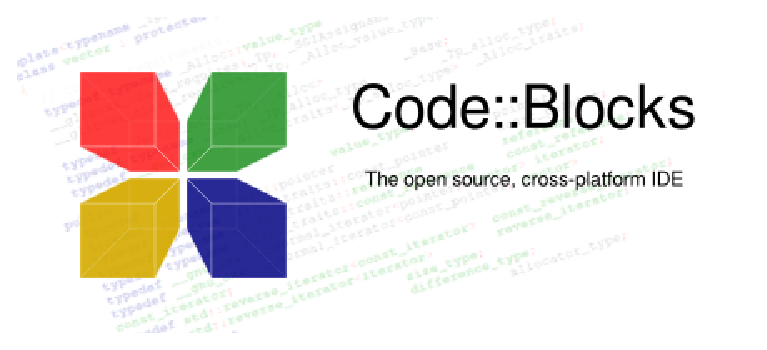
\includegraphics[width=\columnwidth]{mystyles/cb_splash}
    \vfill
    \makeatletter
    \@ifundefined{Subtitle}{%
        {\Huge\textbf{\Subject}\\ [2ex] \Title\\ [2ex] \large{Version \DocVersion}\\ [2ex]}
    }{%
        {\Huge\textbf{\Subject}\\ [2ex] \Title\\ \Subtitle\\ [2ex] \large{Version \DocVersion}\\ [2ex]}
    }
    \makeatother
    \vfill
    Thanks to the \codeblocks team:\\

    Anders F. Bj\"{o}rklund (afb), Biplab Kumar Modak (biplab), Bartomiej wiecki (byo),
    Paul A. Jimenez (ceniza), Koa Chong Gee (cyberkoa), Daniel Orb (daniel2000), Lieven de Cock (killerbot), Yiannis Mandravellos (mandrav), Mispunt (mispunt), Martin Halle (mortenmacfly), Jens Lody (jens), Jerome Antoine (dje), Damien Moore (dmoore),
    Pecan Heber (pecan), Ricardo Garcia (rickg22), Thomas Denk (thomasdenk), tiwag (tiwag), stahta01 (stahta01), Teodor Petrov (oBFusCATed), BlueHazzard (BlueHazzard), Andrew Cottrell (AndrewCot), Miguel Gimenez (wh11204) 

    And many other contributors...

    Original manual in English and in German (V1.x) by Mario Cupelli (mariocup)\\
    Translation in French (v1.x), corrections and additions for version 2 by Gerard Durand (gd\_on).\\
    Some paragraphs are directly imported from \codeblocks WiKi. Don't hesitate to visit \url{https://wiki.codeblocks.org/index.php/Main_Page}, informations are perhaps more up to date.\\

    Permission is granted to copy, distribute and/or modify this document under the terms of the GNU Free Documentation License, Version 1.2 or any later version published by the Free Software Foundation.

    User Manual updated in january 2023
    \end{flushleft}
    \end{titlepage}
    \pagestyle{headings}
%%%%%%%%%%%% Table of contents %%%%%%%%%%%%%%%%%%%%%%%%%%%%%%%%%%%%%%%%%%%
% This ifthenelse is desactivated, because it has problems with recent Miktex versions (22.10), though it was OK with a previous one (22.03).
% More, it's only used when shortdocu is false, which is not the standard case for C::B documentation.
%    \ifthenelse{\boolean{shortdocu}}{}{
%%        \tableofcontents
%        \ifthenelse{\boolean{figreg}}{\listoffigures}{}
%        \ifthenelse{\boolean{tabreg}}{\listoftables}{}
%    }
%    \clearemptydoublepage \pagestyle{headings}
    \pagenumbering{arabic}
}{%
    \begin{titlepage}
        \@ifundefined{Subtitle}{%
            \Huge\textbf{{\Subject} {\Title}}\\
        }{
            \Huge\textbf{{\Subject} {\Title} {\Subtitle}}\\
        }
        \large{Version \DocVersion}
    \end{titlepage}
    \clearemptydoublepage \pagestyle{headings}
    %\tableofcontents
    \clearemptydoublepage \pagenumbering{arabic}
    \pagenumbering{arabic}
}
\makeatother

\ifhtml
	% No tableofcontents
\else
	\tableofcontents{}
\fi
\chapter{\codeblocks Project Management}

The instructions in several paragraphs (for example chapter \pxref{sec:variables_types} or \pxref{sec:plugins}) are official documentations of the \codeblocks Wiki site (eventually reviewed and amended) and available in english only.
This documentation is an extension of the original version 1.1, compiled and/or written by Mario Cupelli.

The below illustration shows the design of the \codeblocks user interface.

\figures[H][width=\columnwidth]{codeblocks}{IDE \codeblocks}

\begin{description}
\item[Management] This window contains the interface \menu{Projects} which will in the following text be referred to as the project view. This view show all the projects opened in \codeblocks at a certain time. The \samp{Symbols} tab of the Management window shows symbols, variables etc..
\item[Editor] In the above illustration, a source named \file{hello.c} is opened with syntax highlighting in the editor.
\item[Open files list] shows a list of all files opened in the editor, in this example: \file{hello.c}.
\item[CodeSnippets] can be displayed via the menu \menu{View,CodeSnippets}. Here you can manage text modules, links to files and links to urls.
\item[Logs \& others]. This window is used for outputting search results, log messages of a compiler etc..
\end{description}

The status bar gives an overview of the following settings:

\begin{itemize}
\item Absolute path of an opened file in the editor.
\item The editor uses the default character encoding of your host operating system. This setting will be displayed with \codeline{default}.
\item Row and column number of the current cursor position in the editor.
\item The configured keyboard mode for inserting text (Insert or Overwrite).
\item Current state of a file. A modified file will be marked with \codeline{Modified} otherwise this entry is empty.
\item The permission of a file. A file with read only settings will display \codeline{Read only} in the status bar. In the window \menu{Open files list} these files will be emphasised with a lock as icon overlay.

\hint{In the active editor the user can select the context menu properties. In the appearing dialog in the tab \menu{General} the option \menu{File is read-only} can be selected. This option will result in a read-only access of the corresponding file within \codeblocks, but the original read and write attributes of the file on the filesystem are not modified.}

\item If you start \codeblocks with the command line option \opt{--personality=\var{profile}} then the status bar will show the currently used profile, otherwise \codeline{default} will be shown. The settings of \codeblocks are stored in the corresponding configuration file \file{\var{personality}.conf}.
\end{itemize}

\codeblocks offers a very flexible and comprehensive project management. The following text will address only some of the features of the project management.

\section{Project View}\label{sec:categories}

In \codeblocks, the sources and the settings for the build process are stored in a project file \file{\var{name}.cbp}. C/C++ sources and the corresponding header files are the typical components of a project. The easiest way to create a new project is  executing the command \menu{File,Project} and selecting a wizard. Then you can add files to the project via the context menu \menu{Add files} in the Management window.

\codeblocks governs the project files in categories according to their file extensions. These are the preset categories:

\begin{description}
\item[Sources] includes source files with the extensions \file{*.c;*.cpp;}.
\item[ASM Sources] includes source files with the extensions \file{*.s;*.S;*.ss;*.asm}.
\item[Headers] includes, among others, files with the extension \file{*.h;}.
\item[Resources] includes files for layout descriptions for wxWidgets windows with the extensions \file{*.res;*.xrc;}. These file types are shown in the \samp{Resources} tab of the Manangement window.
\end{description}

The settings for types and categories of files can be adjusted via the context menu \menu{Project tree,Edit file types \& categories}. Here you can also define custom categories for file extensions of your own. For example, if you wish to list linker scripts with the \file{*.ld} extension in a category called \file{Linkerscript}, you only have to create the new category.

\hint{If you deactivate \menu{Project tree,Categorize by file types} in the context menu, the category display will be switched off, and the files will be listed as they are stored in the file system.}

\section{Notes for Projects}

In \codeblocks, so-called notes can be stored for a project. These notes should contain short descriptions or hints for the corresponding project. By displaying this information during the opening of a project, other users are provided with a quick survey of the project. The display of notes can be switched on or off in the Notes tab of the Properties of a project.

\section{Project Templates}

\codeblocks is supplied with a variety of project templates which are displayed when creating a new project. However, it is also possible to store custom templates for collecting your own specifications for compiler switches, the optimisation to be used, machine-specific switches etc. in templates. These templates will be stored in the \file{Documents and Settings\osp \var{user}\osp Application Data\osp codeblocks\osp UserTemplates} directory in Win 7 (or an equivalent path in the user profile, adapted to each OS). If the templates are to be open to all users, they have to be copied to a corresponding directory of the \codeblocks installation. These templates will then be displayed at the next startup of \codeblocks under \menu{New, Project,User templates}.

\hint{The available templates in the Project Wizard can be edited by selection via right-click.}

\section{Create Projects from Build Targets}

In projects it is necessary to have different variants of the project available. Variants are called Build Targets. They differ with respect to their compiler options, debug information and/or choice of files. A Build Target can also be outsourced to a separate project. To do so, click \menu{Project,Properties}, select the variant from the tab \samp{Build Targets} and click the \samp{Create project from target} button (see \pxref{fig:build_targets}).

\screenshot{build_targets}{Build Targets}

\section{Virtual Targets}

Projects can be further structured in \codeblocks by so-called Virtual Targets. A frequently used project structure consists of two Build Targets, one \samp{Debug} Target which contains debug information and one \samp{Release} Target without this information. By adding Virtual Targets via \menu{Project,Properties,Build Targets} individual Build Targets can be combined. For example, a Virtual Target \samp{All} can create the Targets Debug and Release simultaneously. Virtual Targets are shown in the symbol bar of the compiler under Build Targets.

\section{Pre- and Postbuild steps}\label{sec:pre_postbuild}

\codeblocks makes it possible to perform additional operations before or after compiling a project. These operations are called Prebuilt or Postbuilt Steps. Typical Postbuilt Steps are:

\begin{itemize}
\item Creating an Intel Hexformat from a finished object
\item Manipulating objects by \cmdline{objcopy}
\item Generating dump files by \cmdline{objdump}
\end{itemize}

\genterm{Example}

Creating a Disassembly from an object under Windows. Piping to a file requires calling \cmdline{cmd} with the \opt{/c} option.

\begin{lstlisting}
cmd /c objdump -D name.elf > name.dis
\end{lstlisting}

Archiving a project can be another example for a Postbuilt Step. For this purpose, create a Build Target \samp{Archive} and include the following instruction in the Postbuilt Step:

\begin{lstlisting}
zip -j9 $(PROJECT_NAME)_$(TODAY).zip src h obj $(PROJECT_NAME).cbp
\end{lstlisting}

With this command, the active project and its sources, header and objects will be packed as a zip file. In doing so, the Built-in variables \codeline{$(PROJECT_NAME)} and \codeline{$(TODAY)}, the project name and the current date will be extracted (see \pxref{sec:builtin_variables}). After the execution of the Target \samp{Archive}, the packed file will be stored in the project directory.

In the \file{share/codeblocks/scripts} directory you will find some examples for scripts. You can add a script via menu \menu{Settings,Scripting} and register in a menu. If you execute e.g. the script \file{make\_dist} from the menu then all files belonging to a project will be compressed in an archive \file{\var{project}.tar.gz}.

\section{Adding Scripts in Build Targets}

\codeblocks offers the possibility of using menu actions in scripts. The script represents another degree of freedom for controlling the generation of your project.

\hint{A script can also be included at a Build Target.}

\section{Workspace and Project Dependencies}

In \codeblocks, multiple projects can be open. By saving open projects via \menu{File,Save workspace} you can collect them in a single workspace under \file{\var{name}.workspace}. If you open \file{\var{name}.workspace} during the next startup of von \codeblocks, all projects will show up again.

Complex software systems consist of components which are managed in different \codeblocks projects. Furthermore, with the generation of such software systems, there are often dependencies between these projects.

\genterm{Example}

A project A contains fundamental functions which are made available to other projects in the form of a library. Now, if the sources of this project are modified, then the library has to be rebuilt. To maintain consistency between a project B which uses the functions and project A which implements the functions, project B has to depend on project A. The necessary information on the dependencies of projects is stored in the relevant workspace, so that each project can be created separately. The usage of dependencies makes it also possible to control the order in which the projects will be generated. The dependencies for projects can be set via the selecting the menu \menu{Project,Properties} and then clicking the \samp{Project's dependencies} button.

\section{Including Assembler files}

In the Management window of the Project View, Assembler files are shown in the \file{ASM Sources} category. The user can change the listing of files in categories (see \pxref{sec:categories}). Right-clicking one of the listed Assembler files will open a context menu. Select \menu{Properties} to open a new window. Now select the \samp{Build} tab and activate the two fields \samp{Compile file} and \samp{Link file}. Then select the \samp{Advanced} tab and execute the following steps:

\begin{enumerate}
\item Set \samp{Compiler variable} to CC
\item Select the compiler under \samp{For this compiler}
\item Select \samp{Use custom command to build this file}
\item In the window, enter:
\begin{lstlisting}
$compiler $options $includes <asopts> -c $file -o $object
\end{lstlisting}
\end{enumerate}

The \codeblocks variables are marked by \codeline{$} (see \pxref{sec:command_macros}). They are set automatically so that you only have to replace the Assembler option \var{asopt} by your own settings.

\section{Editor and Tools}

This section describe tools in the éditor window.

\subsection{Default Code}

The company's Coding Rules require source files to have a standard design. \codeblocks makes it possible to include a predefined content at the beginning of a file automatically when creating new C/C++ sources and headers. This predefined content is called default code. This setting can be selected under \menu{Settings,Editor} Default Code. If you create a new file then a macro expansion of variables, e.g. defined via menu \menu{Settings,Global variables},  is performed. A new file can be created via the menu \menu{File,New,File}.

\genterm{Example}

\begin{lstlisting}
/***************************************************************
 *  Project: $(project)
 *  Function:
 ***************************************************************
 *  $Author: mario $
 *  $Name:  $
 ***************************************************************
 *
 *  Copyright 2007 by company name
 *
 ***************************************************************/
\end{lstlisting}

\subsection{Abbreviation}\label{sec:abbreviation}

A lot of typing can be saved in \codeblocks by defining abbreviation. This is done by selecting \menu{Settings,Editor} and defining the abbreviations under the name \var{name}, which can then be called by the keyboard shortcut Ctrl-J (see \pxref{fig:abbreviation}).

\screenshot{abbreviation}{Defining abbreviations}

Parametrisation is also possible by including variables \codeline{$(NAME}) in the abbreviations.

\begin{lstlisting}
#ifndef $(Guard token)
#define $(Guard token)
#endif // $(Guard token)
\end{lstlisting}

When performing the abbreviation \var{name} in the source text and performing Ctrl-J, the content of the variable is requested and included.
%Inherit Class
%Im Editor kann durch Auswahl von Inherit Class \"{u}ber die rechte Maustaste. ???

\subsection{Personalities}\label{sec:personalities}

\codeblocks settings are saved as application data in a file called \file{\var{user}.conf} in the \file{codeblocks} directory. This configuration file contains information such as the last opened projects, settings for the editor, display of symbol bars etc. By default, the \samp{default} personality is set so that the configuration is stored in the file \file{default.conf}. If \codeblocks is called from the command line with the parameter \cmdline{--personality=myuser}, the settings will be stored in the file \file{myuser.conf}. If the profile does not exist already, it will automatically be created. This procedure makes it possible to create the corresponding profiles for different work steps. If you start \codeblocks from the command line with the additional parameter\cmdline{--personality=ask}, a selection box will be displayed for all the available profiles.

\hint{The name of the current profile/personality is displayed in the right corner of the status bar.}

\subsection{Configuration Files}

The \codeblocks settings are stored in the \file{default.conf} profile in the \file{codeblocks} directory of your Application Data. When using personalities (see \pxref{sec:personalities}), the configuration details will be stored in the \file{\var{personality}.conf} file.

The tool \cmdline{cb\_share\_conf}, which can be found in the \codeblocks installation directory, is used for managing and storing these settings.

If you wish to define standard settings for several users of a computer, the configuration file \file{default.conf} has to be stored in the directory \file{\osp Documents and Settings\osp Default User\osp Application Data\osp codeblocks}. During the first startup, \codeblocks will copy the presettings from \samp{Default User} to the application data of the current users.

To create a portable version of \codeblocks on a USB stick, proceed as follows. Copy the \codeblocks installation to a USB stick and store the configuration file \file{default.conf} in this directory. The configuration will be used as a global setting. Please take care that the file is writeable, otherwise changes of the configuration cannot be stored.

\subsection{Navigate and Search}

In \codeblocks there are different ways of quick navigation between files and functions. Setting bookmarks is a typical procedure. Via the shortcut Ctrl-B a bookmark is set or deleted in the source file. Via Alt-PgUp you can jump to the previous bookmark, and via Alt-PgDn you can jump to the next bookmark.

If you select the workspace or a project in the workspace in the project view you will be able to search for a file in the project. Just select \menu{Find file} from the context menu, then type the name of the file and the file will be selected. If you hit return this file will be opened in the editor (see \pxref{fig:project_find_file}).

\screenshot[H][width=.45\columnwidth]{project_find_file}{Searching for files}

In \codeblocks you can easily navigate between header/source files like:

\begin{enumerate}
\item Set cursor at the location where a header file is included and open this file via the context menu \menu{open include file} (see \pxref{fig:open_header})
\item Swap between header and source via the context menu \menu{Swap header/source}
\item Select e.g. a define in the editor and choose \menu{Find declaration} from the context menu to open the file with its declaration.
\end{enumerate}

\screenshot{open_header}{Opening of a header file}

\codeblocks offeres several ways of searching within a file or directory. The dialogue box for searching is opened via \menu{Search,Find} (Ctrl-F) or \menu{Find in Files} (Ctrl-Shift-F).

Alt-G and Ctrl-Alt-G are another useful functions. The dialogue which will open on using this shortcut, lets you select files/functions and then jumps to the implementation of the selected function (see \pxref{fig:select_function}) or opens the selected file in the editor. You may use wildcards like \codeline{*} or \codeline{?} etc. for an incremental search in the dialog.

\screenshot[!hbt][width=.5\columnwidth]{select_function}{Search for functions}

\hint{With the Ctrl-PgUp shortcut you can jump to the previous function, and via Ctrl-PgDn you can jump to the next function.}

In the editor, you can open a new Open Files dialog via Ctrl-Tab and you can switch between the listed entries. If the Ctrl-key is pressed, then a file can be selected in different ways:

\begin{enumerate}
\item If you select an entry with the left mouse button, then the selected file will be opened.
\item If you press the Tab-key you will switch between the listed entries. Releasing the Crtl-key will open the selected file.
\item If you move the mouse over the listed entries, then the current selection will be highlighted. Releasing the Crtl-key will open the selected file.
\item If the mouse pointer is  outside the highlighted selection, then you can use the mouse-wheel to switch between the entries. Releasing the Crtl-key will open the selected file.
\end{enumerate}

A common procedure when developing software is to struggle with a set of functions which are implemented in different files. The Browse Tracker plugin will help you solve this problem by showing you the order in which the files were selected. You can then comfortably navigate the function calls (see \pxref{sec:browsetracker}).

The display of line numbers in \codeblocks can be activated via \menu{Settings,General Settings} in the field \samp{Show line numbers}. The shortcut Ctrl-G or the menu command \menu{Search,Goto line} will help you jump to the desired line.

\hint{If you hold the Ctrl key and then select text in the \codeblocks editor you can perform e.g. a Google search via the context menu.}

\subsection{Symbol view}

The \codeblocks Management window offers a tree view for symbols of C/C++ sources for navigating via functions or variables. As the scope of this view, you can set the current file or project, or the whole workspace.

\hint{Entering a search term or symbol names in the 'Search' input mask of the Symbol Browser results in a filtered view of the symbols if any hits occurred.}

The following categories exist for the symbols:

\begin{description}
\item[Global functions] Lists the implementation of global functions.
\item[Global typedefs] Lists the use of \codeline{typedef} definitions.
\item[Global variables] Displays the symbols of global variables.
\item[Preprocessor symbols] Lists the pre-processor directives created by \codeline{#define}.
\item[Global macros] Lists macros of pre-processor directives.
\end{description}

\figures[H][width=.3\columnwidth]{symbols}{Symbol view}

Structures and classes are displayed in the \menu{bottom tree} and the sort sequence can be modified via the context menu. If a category is selected by mouse-click, the found symbols will be displayed in the lower part of the window (see \pxref{fig:symbols}). Double-clicking the symbol will open the file in which the symbol is defined or the function implemented, and jumps to the corresponding line. An auto-refresh of the symbol browser without saving a file, can be activated via the menu  \menu{Settings,Editor,Code Completion} (see \pxref{fig:cc_realtime_parsing}). For projects with many symbols the performance within \codeblocks will be affected.

\figures[H][width=.85\columnwidth]{cc_realtime_parsing}{Enable real-time parsing}

\hint{In the editor, a list of the classes can be displayed via the context menus \menu{Insert Class method declaration implementation} or \menu{All class methods without implementation}.}

\subsection{Including external help files}

\codeblocks comes with just its own help file: normally, developers need much more help and reference for language, libraries, protocols, file formats and so on. The help plugin makes all the needed documentation available from within \codeblocks itself. Virtually any document can be integrated in the \codeblocks help system, since the help plugin has the ability to launch external programs, if necessary, to view the added documents.

Once added a new help file or document, there will be a new entry in the "Help" menu to open it.
 
The \codeblocks development environment supports the inclusion of external help files via the menu \menu{Settings,Environment}. Include the manual of your choice in the chm format in \menu{Help Files} select \samp{this is the default help file} (see \pxref{fig:help_files}). The entry \codeline{$(keyword)} is a placeholder for a select item in your editor. Now you can select a function in an opened source file in \codeblocks by mouse-click, and the corresponding documentation will appear while pressing F1.

If you have included multiple help files, you can select a term in the editor and choose a help file from the context menu \menu{Locate in} for \codeblocks to search in.

\screenshot{help_files}{Settings for help files}

In \codeblocks you can add even support for man pages. Just add a entry \menu{man} and specify the path as follows.

\begin{lstlisting}
man:/usr/share/man
\end{lstlisting}

On Linux, man pages are usually installed anyway, for Windows you might want to download them e.g. from here: \url{http://www.win.tue.nl/~aeb/linux/man}

\textbf{Helpfile options}

\begin{itemize}
\item You can tell \codeblocks to use a file as the default helpfile, checking the "This is the default help file" box. This way, that file will be shown whenever you press the 'F1' key. Moreover, if you write the \$(keyword) as default keyword (see below), this file will be searched for keywords (taking the word selected or the word below the cursor in the current surce file) and will be opened showing the corresponding topic, if present.

\item You can tell \codeblocks to open the helpfile on a topic of your choice, writing the correspondent keyword in the "Default keyword value" textbox. If the helpfile is the default helpfile and you use \$(keyword) as default keyword, the editor will use the word under the cursor (or currently selected) in the current opened file as keyword, opening the default help file at the relevant topic. This will be true, however, only for the default helpfile: any other helpfile or document will not be searched this way. For example, if you have the language reference as default helpfile and add the standard library helpfile, you will have the language keyword explained when hitting 'F1' on them, but won't have the library functions explained this way. Viceversa, setting the standard library helpfile as default will give you the F1 help on them but you will loose this feature for the language keywords.

\item If your helpfile is an HTML file, you can tell \codeblocks to open it with the embedded HTML viewer, checking the corresponding option.
\end{itemize}

\codeblocks provides an \samp{Embedded HTML Viewer}, which can be used to display simple html file and find keywords within this file. Just configure the path to the html file, which should be parsed and enable the checkbox \menu{Open this file with embedded help viewer} via the menu \menu{Settings,Environment,Help Files}.

\screenshot{embedded_html_viewer}{Embedded HTML Viewer}

\hint{If you select a html file with a double-click within the file explorer (see \pxref{sec:file_explorer}) then the embedded html viewer will be started, as long as no association for html files is made in file extensions handler.}

\textbf{CHM Files}

You can find c++ chm help files on the web. Just add them via the dialog.

For Linux you have to install a chm viewer to be able to open chm files. There are severals like gnochm, kchmviewer, xchm and so on. 

% \section{Scripting}
%
% \codeblocks in Console Modus + Scripts

\subsection{Including external tools}

Including external tools is possible in \codeblocks via \menu{Tools,Configure Tools,Add}. Built-in variables (see \pxref{sec:builtin_variables}) can also be accessed for tool parameters. Furthermore there are several kinds of launching options for starting external applications. Depending on the option, the externally started applications are stopped when \codeblocks is quit. If the applications are to remain open after quitting \codeblocks, the option \menu{Launch tool visible detached} must be set.

\section{Tips for working with \codeblocks}

In this chapter we will present some useful settings in \codeblocks.

\subsection{Tracking of Modifications}

\codeblocks provides a feature to track modifications within a source file and to show a bar in the margin for the changes. Modifications are marked with a yellow changebar and modifications that are already saved will use a green changebar (see \pxref{fig:changebar}). You can navigate between your changes via the menu \menu{Search,Goto next changed line} or \menu{Search,Goto previous changed line}. The same functionality is also accessible via the shortcuts Ctrl-F3 and Ctrl-Shift-F3.

\screenshot{changebar}{Tracking of modifications}

This feature can be enabled or disabled with the checkbox \menu{Use Changebar} in the menu \menu{Settings,Editor,Margins and caret}.

\hint{If a modified file is closed, then the changes history like undo/redo and changebars get lost. Via the menu \menu{Edit,Clear changes history} or the corresponding context menu you are able to clear the changes history even if the file is kept open.}

\subsection{Data Exchange with other applications}

Data can be exchanged between \codeblocks and other applications. For this interprocess communication DDE (Dynamic Data Exchange) is used for windows and under different operating systems it is a TCP based communication.

With this interface different commands with the following syntax can be sent to a \codeblocks instance.

\begin{lstlisting}
[<command>("<parameter>")]
\end{lstlisting}

These commands are currently available:

\begin{description}
\item[Open] The command

\begin{lstlisting}
[Open("d:\temp\test.txt")]
\end{lstlisting}

uses the parameter, in our case it is a file specified with an absolute path, and opens it in an existing \codeblocks instance or starts a first instance if required.
\item[OpenLine] This command opens a file at a given line number in a \codeblocks instance. The line number is specified with \codeline{:line}.

\begin{lstlisting}
[OpenLine("d:\temp\test.txt:10")]
\end{lstlisting}

\item[Raise] Set the focus to the \codeblocks instance. A parameter must not be passed.
\end{description}

\subsection{Configuring environmental variables}\label{sec:EnvVars_Cfg}

See also "Environment Variables Plugin" in \pxref{sec:EnvVar_Plugin}.

The configuration for an operating system is specified by so-called environmental variables. The environmental variable \codeline{PATH} for example contains the path to an installed compiler. The operating system will process this environmental variable from beginning to end, i.e. the entries at the end will be searched last. If different versions of a compiler or other applications are installed, the following situations can occur:

\begin{itemize}
\item An incorrect version of a software is called
\item Installed software packages call each other
\end{itemize}

So it might be the case that different versions of a compilers or other tools are mandatory for different projects. One possibility in such a case is to change the environmental variables in the system control for every project. However, this procedure is error-prone and not flexible. For this requirement, \codeblocks offers an elegant solution. Different configurations of environmental variables can be created which are used only internally in \codeblocks. Additionally, you can switch between these configurations. The \pxref{fig:env_variables} shows the dialogue which you can open via \samp{Environment Varibales} under \menu{Settings,Environment}. A configuration is created via the \samp{Create} button.

\screenshot{env_variables}{Environmental variables}

Access and scope of the environmental variables created here, is limited to \codeblocks. You can expand these environmental variables just like other \codeblocks variables via \codeline{$(NAME)}.

\hint{A configuration for the environmental variable for each project can be selected in the context menu \menu{Properties} of the \samp{EnvVars options} tab.}

\genterm{Example}

You can write the used environment into a postbuild Step (see \pxref{sec:pre_postbuild}) in a file \file{\var{project}.env} and archive it within your project.

\begin{lstlisting}
cmd /c echo \%PATH\%  > project.env
\end{lstlisting}

or under Linux

\begin{lstlisting}
echo \$PATH > project.env
\end{lstlisting}

\subsection{Switching between perspectives}

Depending on the task in hand, it can be useful to have different configurations or views in \codeblocks and to save these configurations/views. By default, the settings (e. g. show/hide symbol bars, layout, etc.) are stored in the \file{default.conf} configuration file. By using the command line option \opt{--personality=ask} during the start of \codeblocks, different settings can be selected. Apart from this global setting, a situation might occur where you wish to switch between different views of windows and symbol bars during a session. Editing files and debugging projects are two typical examples for such situations. \codeblocks offers a mechanism for storing and selecting different perspectives to prevent the user from frequently having to open and close windows and symbol bars manually. To save a perspective, select the menu \menu{View,Perspectives,Save current} and enter a name at \var{name}. The command \menu{Settings,Editor,Keyboard shortcuts,View,Perspectives,\var{name}} allows a keyboard shortcut to be defined for this process. This mechanism makes it possible to switch between different views by simply using hot keys.

\hint{Another example is editing a file in Full Screen mode without symbol bars. You can create a perspective such as \samp{Full} and assign a hot key for this purpose.}

\subsection{Switching between projects}

If several projects or files are opened at the same time, the user needs a way to switch quickly between the projects or files. \codeblocks has a number of shortcuts for such situations.

\begin{description}
\item[Alt-F5] Activates the previous project from the project view.
\item[Alt-F6] Activates the next project from the project view.
\item[F11] Switches within the editor between a source file \file{\var{name}.cpp} and the corresponding header file \file{\var{name}.h}
\end{description}

\subsection{Extended settings for compilers}

During the build process of a project, the compiler messages are displayed in the Messages window in the Build Log tab. If you wish to receive detailed information, the display can be extended. For this purpose click \menu{Settings,Compiler and Debugger} and select \samp{Other Settings} in the drop-down field.

\screenshot{compiler_debugger}{Setting detail information}

Take care that the correct compiler is selected. The \samp{Full command line} setting in the Compiler Logging field outputs the complete information in the Build Log. In addition, this output can be logged in a HTML file. For this purpose select \samp{Save build log to HTML file when finished}.
Furthermore, \codeblocks offers a progress bar for the build process in the Build Log window which can be activated via the \samp{Display build progress bar} setting.

\subsection{Zooming within the editor}

\codeblocks offers a very efficient editor. This editor allows you to change the size in which the opened text is displayed. If you use a mouse with a wheel, you only need to press the Ctrl key and scroll via the mouse wheel to zoom in and out of the text.

\hint{With the shortcut Ctrl-Numepad-/ or with the menu \menu{Edit,Special commands,Zoom,Reset} the original font size of the active file in the editor is restored.}

\subsection{Wrap Mode}

When editing text files, e. g. \file{*.txt}, within \codeblocks, it might be useful to have the text wrapped, meaning long lines will be displayed in several lines on the screen so that they can be properly edited. The \samp{Word wrap} function can be activated via \menu{Settings,Editor,Other Options} or by setting the checkbox \menu{Word wrap}. The Home and End keys position the cursor at the beginning or end of wrapped lines respectively. When setting \menu{Settings,Editor,Other Options} and \menu{Home key always move to caret to first column}, the cursor will be positioned at the beginning or end of the current line respectively, if the Home or End keys are pressed. If positioning the cursor at the beginning of the first line of the current paragraph is desired, the key combination \menu{Alt-Home} is to be used. The same applies analogously for \menu{Alt-End} for positioning the cursor at the end of the last line of the current paragraph.

\subsection{Select modes in editor}

\codeblocks supports different modes for selecting or pasting of strings.

\begin{enumerate}
\item With the left mouse button a text in the active editor can be selected and then the mouse button can be released. With the mouse wheel the user can scroll to a position. If the middle mouse button is pressed then the formerly selected text will be inserted. This feature is available per file and can be seen a clipboard per file.
\item Pressing the \samp{ALT} key will activate the so-called block-select mode and a rectangle selection can be raised with the left mouse button. If the Alt key is released this selection can be copied or pasted. This feature is helpful if you want to select some columns e.g. of an array and copy and paste the content.
 \item In the menu \menu{Settings,Editor,Margins and Caret} so-called \menu{Virtual Spaces} can be activated. This option enables that a selection in the block select mode can start or end within an empty line.
\item In the menu  \menu{Settings,Editor,Margins and Caret} the \menu{Multiple Selection} can be activated. While holding the Ctrl-key the user can select different lines in the active editor via the left mouse button. The selections will be appended in the clipboard via the shortcut  Ctrl-C or Ctrl-X. Ctrl-V will insert the content at the current cursor position. An additional option  called \menu{Enable typing (and deleting)}  can be activated for multiple selections. This feature is useful if you want to add a pre-processor directive like \codeline{#ifdef} at different source lines or if you want to overwrite or replace a text at several positions.
\end{enumerate}

\hint{Most Linux window managers use ALT-LeftClickDrag to move a window, so you will have to disable this window manager behavior first for block select to work.}

\subsection{Code folding}

\codeblocks supports so called code folding. With this feature you can fold e.g. functions within the \codeblocks editor. A folding point is marked by minus symbol in the left margin of
the editor view. In the margin the beginning and the end of a folding point is visible as vertical line. If you click the minus symbol with the left mouse button the code snippet will be folded or unfolded. Via the menu \menu{Edit,Folding} you can select the folding. In the editor you see folded code as continous horizontal line.

\hint{The folding style and the folding depth limit can be configured via menu \menu{Settings,Editor,Folding}.}

\codeblocks provides the folding feature also for preprocessor directives. To enable this feature select \samp{Fold preprocessor commands} via the menu \menu{Settings,Editor} in the folding entry.

Another possibility is to set user defined folding points. The start of folding point is entered as comment with a opening bracket and the end is market with a comment with a closing bracket.

\begin{verbatim}
//{
code with user defined folding
//}
\end{verbatim}

\subsection{Auto complete}

If you open a project in \codeblocks the \samp{Search directories} of your compiler and the project, the sources and headers of your project are parsed. In addition the keywords of the corresponding lexer file are parsed. The parse information is used for the auto complete feature in \codeblocks. Please check the settings for the editor if this feature is enabled. The auto completion is accessible with the shortcut Ctrl-Space. Via the menu \menu{Settings,Editor,Syntax highlighting} you can add user defined keywords to your lexer.

\subsection{Find broken files}

If a file is removed from disk, but is still included in the project file \file{\var{project}.cbp}, then this \samp{broken file} will be shown a broken symbol in the project view. You should use the menu \menu{Remove file from project} instead of deleting files.

In large projects with a lot of subdirectories the search for broken files can be time consuming. \codeblocks offers with the plug-in ThreadSearch (see \pxref{sec:thread_search}) a simple solution for this problem. If you enter a search expression in ThreadSearch and select the option \menu{Project files} or \menu{Workspace files}, then ThreadSearch will parse all files that are included in a project or workspace. If a broken file is found ThreadSerch will issue an error with the missing file.

\subsection{Including libraries}

In the build options of a project, you can add the used libraries via the \samp{Add} button in the \samp{Link libraries} entry of the \samp{Linker Settings}. In doing so, you can either use the absolute path to the library or just give the name without the \file{lib} prefix and file extension.

\genterm{Example}

For a library called \file{\var{path}\osp libs\osp lib\var{name}.a}, just write \file{\var{name}}. The linker with the corresponding search paths will then include the libraries correctly.

\hint{Another way to include libraries is documented in \pxref{sec:lib_finder}.}

\subsection{Object linking order}

During compiling, objects \file{name.o} are created from the sources \file{name.c/cpp}. The linker then binds the individual objects into an application \file{name.exe} or for the embedded systems \file{name.elf}. In some cases, it might be desirable to predefine the order in which the objects will be linked. In \codeblocks, this can be achieved by assigning priorities. In the context menu \menu{Properties}, you can define the priorities of a file in the Build tab. A low priority will cause the file to be linked earlier.

\subsection{Autosave}

\codeblocks offers ways of automatically storing projects and source files, or of creating backup copies. This feature can be activated in the menu \menu{Settings,Environment,Autosave}. In doing so, \samp{Save to .save file} should be specified as the method for creating the backup copy.

\subsection{Settings for file extensions}\label{sec:file_extension}

In \codeblocks, you can choose between several ways of treating file extensions. The settings dialogue can be opened via \menu{Settings,Files extension handling}.
You can either use the applications assigned by Windows for each file extension (open it with the associated application), or change the setting for each extensions in such a way that either a user-defined program will start (launch an external program), or the file will be opened in the \codeblocks editor (open it inside \codeblocks editor).

\hint{If a user-defined program is assigned to a certain file extension, the setting \samp{Disable \codeblocks while the external program is running} should be deactivated because otherwise \codeblocks will be closed whenever a file with this extension is opened.}

\section{\codeblocks at the command line}

IDE \codeblocks can be executed from the command line without a graphic interface. In such a case, there are several switches available for controlling the build process of a project. Since \codeblocks is thus scriptable, the creation of executables can be integrated into your own work processes.

\begin{lstlisting}
codeblocks.exe /na /nd --no-splash-screen --build <name>.cbp --target='Release'
\end{lstlisting}

\begin{description}
\item[\var{filename}] Specifies the project \file{*.cbp} filename or workspace \file{*.workspace} filename. For instance, \var{filename} may be \file{project.cbp}. Place this argument at the end of the command line, just before the output redirection if there is any.
\item[--file=\var{filename}\optional{:line}] Open file in \codeblocks and optionally jump to a specific line.
\item[/h, --help] Shows a help message regarding the command line arguments.
\item[/na, --no-check-associations] Don't perform any file association checks (Windows only).
\item[/nd, --no-dde] Don't start a DDE server (Windows only).
\item[/ni, --no-ipc] Don't start an IPC server (Linux and Mac only).
\item[/ns, --no-splash-screen] Hides the splash screen while the application is loading.
\item[/d, --debug-log] Display the debug log of the application.
\item[--prefix=\var{str}] Sets the shared data directory prefix.
\item[/p, --personality=\var{str}, --profile=\var{str}] Sets the personality to use. You can use ask as the parameter to list all available personalities.
\item[--rebuild] Clean and build the project or workspace.
\item[--build] Build the project or workspace.
\item[--target=\var{str}] Sets target for batch build. For example \cmdline{--target='Release'}.
\item[--no-batch-window-close] Keeps the batch log window visible after the batch build is completed.
\item[--batch-build-notify] Shows a message after the batch build is completed.
\item[--safe-mode] All plugins are disabled on startup.
\item[$>$ \var{build log file}] Placed in the very last position of the command line, this may be used to redirect standard output to log file. This is not a codeblock option as such, but just a standard DOS/*nix shell output redirection.
\end{description}

\section{Shortcuts}

This section describes the shortcuts which are or can be used in \codeblocks.

\subsection{Introduction}

This plugin can be used to bind one or more key shortcuts to the menu items.

Even if an IDE such as \codeblocks is mainly handled by mouse, keyboard shortcuts are nevertheless a very helpful way of speeding up and simplifying work processes. In the below table, we have collected some of the available keyboard shortcuts.

\subsection{Features}
\begin{description}
\item Includes a configuation panel and a complete system to view/remove/add/edit command shortcuts.
\item Supports multiple key profiles and a complete load/save system is present.
\item Allows the users to customize any menu command they want, and define multiple key-shortcut to each command.
\end{description}

\subsection{Usage}

The configuration page for the plugin can be accessed through the \menu{Settings,Editor} menu, and then selecting the Keyboard Shortcuts section.

\screenshot{KeyBindConfig}{Keyboard shortcuts configuration dialog}

Selecting a command, from the Commands tree, shows the current shortcuts for that command on the right. In the picture Open... is selected and the default shortcut Ctrl-O is displayed.

To add a new shortcut, for the selected command, follow these steps:

\begin{enumerate}
\item Place the focus on the text box under New Shortcut and press the keys, for example F3 or Ctrl-A.
\item Check Currently assigned to, if another command already has that shortcut you will see it's name there. If the text says None it's safe.
\item Press Add to add the shortcut on the list.
\item Press OK on the dialog to save changes and return to editor.
\end{enumerate}
    
\subsection{Editor}

{\small
\begin{longtable}{|l|l|}\hline
\textbf{Function}		                    &   \textbf{Shortcut Key}   \\ \hline
\endhead   % To repeat the title line, if needed
Undo last action 	                        &   Ctrl+Z                  \\ \hline
Redo last action 	                        &   Ctrl+ Shift+Z           \\ \hline
Cut selected text                           &   Ctrl+X                  \\ \hline
Copy selected text                          &   Ctrl+C                  \\ \hline
Paste text from clipboard                   &   Ctrl+V                  \\ \hline
Select all text                             &   Ctrl+A                  \\ \hline
Swap header / source 	                    &	F11                     \\ \hline
Comment highlighted code                    &	Ctrl+Shift+C            \\ \hline
Uncomment highlighted code                  & 	Ctrl+Shift+X            \\ \hline
Duplicate line caret is on                  & 	Ctrl+D                  \\ \hline
Auto+complete / Abbreviations               & 	Ctrl+Space/Ctrl+J       \\ \hline
Show call tip 	                            &	Ctrl+Shift+Space        \\ \hline
Swap line caret is on with line above it    &	Ctrl+T                  \\ \hline
Toggle bookmark 	                        &	Ctrl+B                  \\ \hline
Goto previous bookmark 	                    &	Alt+PgUp                \\ \hline
Goto next bookmark 	                        &	Alt+PgDown              \\ \hline
Toggle current block folding 	            &	F12                     \\ \hline
Toggle all folds 	                        &	Shift+F12               \\ \hline
\caption{Basic shortcuts}
\end{longtable}
}

This is a list of shortcuts provided by the \codeblocks editor component. These shortcuts cannot be rebound.

{\small
\begin{longtable}{|l|l|}\hline
\textbf{Function}		                    &   \textbf{Shortcut Key}   \\ \hline
\endhead   % To repeat the title line, if needed
Magnify text size. 	                        &   Ctrl+Keypad "+"         \\ \hline
Reduce text size. 	                        &   Ctrl+Keypad "-"         \\ \hline
Restore text size to normal. 	            &   Ctrl+Keypad "/"         \\ \hline
Cycle through recent files. 	            &   Ctrl+Tab                \\ \hline
Indent block. 	                            &   Tab                     \\ \hline
Dedent block. 	                            &   Shift+Tab               \\ \hline
Delete to start of word. 	                &   Ctrl+BackSpace          \\ \hline
Delete to end of word. 	                    &   Ctrl+Delete             \\ \hline
Delete to start of line. 	                &   Ctrl+Shift+BackSpace    \\ \hline
Delete to end of line. 	                    &   Ctrl+Shift+Delete       \\ \hline
Go to start of document. 	                &   Ctrl+Home               \\ \hline
Extend selection to start of document. 	    &   Ctrl+Shift+Home         \\ \hline
Go to start of display line. 	            &   Alt+Home                \\ \hline
Extend selection to start of display line. 	&   Alt+Shift+Home          \\ \hline
Go to end of document. 	                    &   Ctrl+End                \\ \hline
Extend selection to end of document. 	    &   Ctrl+Shift+End          \\ \hline
Go to end of display line. 	                &   Alt+End                 \\ \hline
Extend selection to end of display line. 	&   Alt+Shift+End           \\ \hline
Expand or contract a fold point. 	        &   Ctrl+Keypad "*"         \\ \hline
Create or delete a bookmark. 	            &   Ctrl+F2                 \\ \hline
Go to next bookmark. 	                    &   F2                      \\ \hline
Select to next bookmark. 	                &   Alt+F2                  \\ \hline
Find selection. 	                        &   Ctrl+F3                 \\ \hline
Find selection backwards. 	                &   Ctrl+Shift+F3           \\ \hline
Scroll up. 	                                &   Ctrl+Up                 \\ \hline
Scroll down. 	                            &   Ctrl+Down               \\ \hline
Line cut. 	                                &   Ctrl+L                  \\ \hline
Line copy. 	                                &   Ctrl+Shift+T            \\ \hline
Line delete. 	                            &   Ctrl+Shift+L            \\ \hline
Line transpose with previous. 	            &   Ctrl+T                  \\ \hline
Line duplicate. 	                        &   Ctrl+D                  \\ \hline
\makecell[l]{Find matching preprocessor conditional, \\
skipping nested ones.} 	                    &   Ctrl+K                  \\ \hline
Select to matching preprocessor conditional.&   Ctrl+Shift+K            \\ \hline
\makecell[l]{Find matching preprocessor conditional backwards, \\
skipping nested ones.} 	                    &   Ctrl+J                  \\ \hline
Select to matching preprocessor conditional backwards. 	&   Ctrl+Shift+J\\ \hline
Previous paragraph. Shift extends selection.&   Ctrl+[                  \\ \hline
Next paragraph. Shift extends selection. 	&   Ctrl+]                  \\ \hline
Previous word. Shift extends selection. 	&   Ctrl+Left               \\ \hline
Next word. Shift extends selection. 	    &   Ctrl+Right              \\ \hline
Previous word part. Shift extends selection.&   Ctrl+/                  \\ \hline
Next word part. Shift extends selection. 	&   Ctrl+\osp               \\ \hline
\caption{Other editor shortcuts}
\end{longtable}
}

\subsection{Files}

{\small 
\begin{longtable}{|l|l|}\hline
\textbf{Function}		        &   \textbf{Shortcut Key}       \\ \hline
\endhead   % To repeat the title line, if needed
New file or project 	        &	Ctrl+N                      \\ \hline
Open existing file or project   &	Ctrl+O                      \\ \hline
Save current file 	            &	Ctrl+S                      \\ \hline
Save all files 		            &	Ctrl+Shift+S                \\ \hline
Close current file 	            &	Ctrl+F4/Ctrl+W              \\ \hline
Close all files 	            &	Ctrl+Shift+F4/Ctrl+Shift+W  \\ \hline
\caption{File shortcuts}
\end{longtable}
}

This is a list of shortcuts provided by the \codeblocks editor component. These shortcuts cannot be rebound.

{\small 
\begin{longtable}{|l|l|}\hline
\textbf{Function}		    &   \textbf{Shortcut Key}   \\ \hline
\endhead   % To repeat the title line, if needed
Activate next open file 	&   Ctrl+Tab                \\ \hline
Activate previous open file &   Ctrl+Shift+Tab          \\ \hline
\caption{Other file shortcuts}
\end{longtable}
}

\subsection{View}

{\small 
\begin{longtable}{|l|l|}\hline
\textbf{Function}		            &   \textbf{Shortcut Key}   \\ \hline
\endhead   % To repeat the title line, if needed
Show / hide Messages pane	        &	F2                      \\ \hline
Show / hide Management pane 	    &	Shift+F2                \\ \hline
Move project up (in Project tree) 	&   Ctrl+Shift+Up           \\ \hline
Move project down (in Project tree) &   Ctrl+Shift+Down         \\ \hline
Activate prior (in Project tree)    & 	Alt+F5                  \\ \hline
Activate next (in Project tree)     &	Alt+F6                  \\ \hline
Zoom in / out 	                    &   Ctrl+Roll Mouse Wheel   \\ \hline
Focus editor 	                    &   CTRL+Alt+E              \\ \hline
\caption{View shortcuts}
\end{longtable}
}

\subsection{Search}

{\small 
\begin{longtable}{|l|l|}\hline
\textbf{Function}		    &   \textbf{Shortcut Key}   \\ \hline
\endhead   % To repeat the title line, if needed
Find 		                &	Ctrl+F                  \\ \hline
Find next 	                &	F3                      \\ \hline
Find previous 	            &	Shift+F3                \\ \hline
Find in files 	            &	Crtl+Shift+F            \\ \hline
Replace 	                &	Ctrl+R                  \\ \hline
Replace in files            &	Ctrl+Shift+R            \\ \hline
Goto line 	                &	Ctrl+G                  \\ \hline
Goto next changed line 	    &	Ctrl+F3                 \\ \hline
Goto previous changed line 	&	Ctrl+Shift+F3           \\ \hline
Goto file 	                &	Alt+G                   \\ \hline
Goto function 	            &	Ctrl+Alt+G              \\ \hline
Goto previous function      &   Ctrl+PgUp               \\ \hline
Goto next function          &   Ctrl+PgDn               \\ \hline
Goto declaration            &   Ctrl+Shift+.            \\ \hline
Goto implementation         &   Ctrl+.                  \\ \hline
Open include file           &   Ctrl+Alt+.              \\ \hline
\caption{Search shortcuts}
\end{longtable}
}

\subsection{Build}

{\small 
\begin{longtable}{|l|l|}\hline
\textbf{Function}		&   \textbf{Shortcut Key}   \\ \hline
\endhead   % To repeat the title line, if needed
Build 		            &	Ctrl+F9                 \\ \hline
Compile current file	&	Ctrl+Shift+F9           \\ \hline
Run		                &	Ctrl+F10                \\ \hline
Build and Run 	        &	F9                      \\ \hline
Rebuild 	            &	Ctrl+F11                \\ \hline
\caption{Build shortcuts}
\end{longtable}
}

\subsection{Debug}

{\small 
\begin{longtable}{|l|l|}\hline
\textbf{Function}		    &   \textbf{Shortcut Key}   \\ \hline
\endhead   % To repeat the title line, if needed
Debug 	                    &   F8                      \\ \hline
Continue debugging 	        &   Ctrl+F7                 \\ \hline
Step over a code block 	    &   F7                      \\ \hline
Step into a code block 	    &   Shift+F7                \\ \hline
Step out of a code block 	&   Ctrl+Shift+F7           \\ \hline
Toggle breakpoint 	        &   F5                      \\ \hline
Run to cursor 	            &   F4                      \\ \hline
Previous error 	            &   Alt+F1                  \\ \hline
\caption{Debug shortcuts}
\end{longtable}
}

\chapter{Plugins}\label{sec:plugins}

Most of the plugins described ib this chapter are also in the Wiki. Texts and figures have been copied from the Wiki but adapted to be included in Latex documents (Miktex 2.9).

\section{General}

\codeblocks' features can be extend by using plugins. There are generally three types of plugins:
\begin{description}
\item[Core plugins:] developed and maintained by the core C::B team.
\item[Contrib plugins:] developed and maintained by the community and proven to be very valuable. So they are integrated into the C::B SVN.
\item[3rd party plugins:] developed and maintained by the community but not (yet?) in the C::B repository. Theses plugins often have their own repository or are being posted (including the source code) in the forums.
\end{description}

\textbf{If you are looking for plugins}:
\begin{enumerate}
\item Look in the official release. Notice that the installer / package manager might require you to enable some of the plugins specifically. So READ carefully.
\item Search the forums for announcements, especially the forums at \url{https://forums.codeblocks.org/index.php/board,14.0.html}.
\item There might be information on the Wiki concerning other plugins on this page and here : \url{https://wiki.codeblocks.org/index.php/Announcement_for_plugins/patches}.
\end{enumerate}

For Windows users, the default behavior of the current installer does \textbf{not} install contrib plugins. You need to manually check the "contrib plugin" checkbox when asked for selected components to install. There is no way to install them manually afterwards.


\textbf{If you are developing plugins}: Surely you can work with plugin as you like, but here are some suggestions:

\tab Announce them in the plugin development board in the forums - including the (initial) source code.

OR

\tab Setup your own webpage (or use a file sharing platform) and post the link to the sources/binaries/svn access in the plugin development board in the forums.

OR

\tab Setup a repository, probably at BerliOS or SourceForge, post the link to the sources/binaries/svn access in the plugin development board in the forums. Notice: This is very convenient as attachments in our forum might be deleted from time to time. So it is not safe to post source code in the forums.

THEN

\tab Enter the plugins description on this page.

\tab Announce the plugin using this template on \url{https://wiki.codeblocks.org/index.php/Template_for_plugin_announcement}

\begin{ASTYLE}
\section{Astyle}\label{sec:astyle}

Artistic Style is a source code indenter, source code formatter, and source code beautifier for the C, C++, C\# programming languages. It can be used to select different styles of coding rules within \codeblocks.

\screenshot{astyle}{Formating your source code}

When indenting source code, we as programmers have a tendency to use both spaces and tab characters to create the wanted indentation. Moreover, some editors by default insert spaces instead of tabs when pressing the tab key, and other editors have the ability to prettify lines by automatically setting up the white space before the code on the line, possibly inserting spaces in a code that up to now used only tabs for indentation.

Since the number of space characters shown on screen for each tab character in the source code changes between editors, one of the standard problems programmers are facing when moving from one editor to another is that code containing both spaces and tabs that was up to now perfectly indented, suddenly becomes a mess to look at when changing to another editor. Even if you as a programmer take care to ONLY use spaces or tabs, looking at other people's source code can still be problematic.

To address this problem, Artistic Style was created - a filter written in C++ that automatically re-indents and re-formats C / C++ / C\# source files.

\hint{When copying code, for example from the internet or a manual, this code will automatically be adapted to the coding rules in \codeblocks.}

\end{ASTYLE}

\begin{AUTOVERSIONING}
\section{AutoVersioning}\label{sec:autoversioning}

An application versioning plug in that increments the version and build number of your application every time a change has been made and stores it in \file{version.h} with easy to use variable declarations. Also have a feature for committing changes a la SVN style, a version scheme editor, a change log generator and more $\ldots$

\subsection{Introduction}

The idea of the AutoVersioning plugin was made during the development of a pre-alpha software that required the version info and status. Been to busy coding, without time to maintain the version number, just decided to develop a plugin that could do the job with little intervention as possible.

\subsection{Features}

Here is the list of features the plugin covers summarized:

\begin{itemize}
\item Supports C and C++.
\item Generates and auto increment version variables.
\item Software status editor.
\item Integrated scheme editor for changing the behavior of the auto incrementation of version values.
\item Date declarations as month, date and year.
\item Ubuntu style version.
\item Svn revision check.
\item Change log generator.
\item Works on Windows and Linux.
\end{itemize}

\subsection{Usage}

Just go to \menu{Project,Autoversioning} menu. A pop up window like this will appear:

\figures[H][width=.45\columnwidth]{autoversion_configure}{Configure project for Autoversioning}

When hitting yes on the ask to configure message box, the main auto versioning configuration dialog will open, to let you configure the version info of your project.

After configuring your project for auto versioning, the settings that you entered on the configuration dialog will be stored on the project file, and a \file{version.h} file will be created. For now, every time that you hit the \menu{Project,Autoversioning} menu the configuration dialog will popup to let you edit your project version and versioning related settings, unless you don't save the new changes made by the plugin to the project file.

\subsection{Dialog notebook tabs}
\genterm{Version Values}

Here you just enter the corresponding version values or let the auto versioning plugin increment them for you (see \pxref{fig:autoversion_editor}).

\begin{description}
\item[Major] Increments by 1 when the minor version reaches its maximum
\item[Minor] Increments by 1 when the build number pass the barrier of build times, the value is reset to 0 when it reach its maximum value.
\item[Build Number] (also equivalent to Release) - Increments by 1 every time that the revision number is incremented.
\item[Revision] Increments randomly when the project has been modified and then compiled.
\end{description}

\screenshot{autoversion_editor}{Set Version Values}

\genterm{Status}

Some fields to keep track of your software status with a list of predefined values for convenience(see \pxref{fig:autoversion_status}).

\begin{description}
\item[Software Status] The typical example should be v1.0 Alpha
\item[Abbreviation] Same as software status but like this: v1.0a
\end{description}

\screenshot{autoversion_status}{Set Status of Autoversioning}

\genterm{Scheme}

Lets you edit how the plugin will increment the version values (see \pxref{fig:autoversion_scheme}).

\screenshot{autoversion_scheme}{Scheme of autoversioning}

\begin{description}
\item[Minor maximum] The maximum number that the Minor value can reach, after this value is reached the Major is incremented by 1 and next time project is compiled the Minor is set to 0.
\item[Build Number maximum] When the value is reached, the next time the project is compiled is set to 0. Put a 0 for unlimited.
\item[Revision maximum] Same as Build Number maximum. Put a 0 for unlimited
\item[Revision random maximum] The revision increments by random numbers that you decide, if you put here 1, the revision obviously will increment by 1.
\item[Build times before incrementing Minor] After successful changes to code and compilation the build history will increment, and when it reaches this value the Minor will increment.
\end{description}

\genterm{Settings}

Here you can set some settings of the auto versioning behavior (see \pxref{fig:autoversion_settings}).

\screenshot{autoversion_settings}{Settings of Autoversioning}

\begin{description}
\item[Autoincrement Major and Minor] Lets the plugin increments this values by you using the scheme. If not marked only the Build Number and Revision will increment.
\item[Create date declarations] Create entries in the \file{version.h} file with dates and ubuntu style version.
\item[Do Auto Increment] This tells the plugin to automatically increment the changes when a modification is made, this incrementation will occur before compilation.
\item[Header language] Select the language output of \file{version.h}
\item[Ask to increment] If marked, Do Auto Increment, it ask you before compilation (if changes has been made) to increment the version values.
\item[svn enabled] Search for the svn revision and date in the current folder and generates the correct entries in \file{version.h}
\end{description}

\genterm{Changes Log}

This lets you enter every change made to the project to generate a \file{ChangesLog.txt} file (see \pxref{fig:autoversion_changelog}).

\screenshot{autoversion_changelog}{Changelog of Autoversioning}

\begin{description}
\item[Show changes editor when incrementing version] Will pop up the changes log editor when incrementing the version.
\item[Title Format] A format able title with a list of predefined values.
\end{description}

\subsection{Including in your code}

To use the variables generated by the plugin just \codeline{\#include <version.h>}. An example code would be like the following:

\begin{lstlisting}
#include <iostream>
#include "version.h"

void main(){
    std::cout<<AutoVersion::Major<<endl;
}
\end{lstlisting}

\genterm{Output of version.h}

The generated header file. Here is a sample content of the file on c++ mode:

\begin{lstlisting}
#ifndef VERSION_H
#define VERSION_H

namespace AutoVersion{

	//Date Version Types
	static const char DATE[] = "15";
	static const char MONTH[] = "09";
	static const char YEAR[] = "2007";
	static const double UBUNTU_VERSION_STYLE = 7.09;

	//Software Status
	static const char STATUS[] = "Pre-alpha";
	static const char STATUS_SHORT[] = "pa";

	//Standard Version Type
	static const long MAJOR = 0;
	static const long MINOR = 10;
	static const long BUILD = 1086;
	static const long REVISION = 6349;

	//Miscellaneous Version Types
	static const long BUILDS_COUNT = 1984;
	#define RC_FILEVERSION 0,10,1086,6349
	#define RC_FILEVERSION_STRING "0, 10, 1086, 6349\0"
	static const char FULLVERSION_STRING[] = "0.10.1086.6349";

}
#endif //VERSION_h
\end{lstlisting}

On C mode is the same as C++ but without the namespace:

\begin{lstlisting}
#ifndef VERSION_H
#define VERSION_H

	//Date Version Types
	static const char DATE[] = "15";
	static const char MONTH[] = "09";
	static const char YEAR[] = "2007";
	static const double UBUNTU_VERSION_STYLE = 7.09;

	//Software Status
	static const char STATUS[] = "Pre-alpha";
	static const char STATUS_SHORT[] = "pa";

	//Standard Version Type
	static const long MAJOR = 0;
	static const long MINOR = 10;
	static const long BUILD = 1086;
	static const long REVISION = 6349;

	//Miscellaneous Version Types
	static const long BUILDS_COUNT = 1984;
	#define RC_FILEVERSION 0,10,1086,6349
	#define RC_FILEVERSION_STRING "0, 10, 1086, 6349\0"
	static const char FULLVERSION_STRING[] = "0.10.1086.6349";

#endif //VERSION_h
\end{lstlisting}

\subsection{Change log generator}

This dialog is accessible from the menu \menu{Project,Changes Log}. Also if checked Show changes editor when incrementing version on the changes log settings, the window will open to let you enter the list of changes after a modification to the project sources or an incrementation event (see \pxref{fig:autoversion_changes}).

\screenshot{autoversion_changes}{Changes for a project}

\genterm{Buttons Summary}

\begin{description}
\item[Add] Appends a row in to the data grid
\item[Edit] Enables the modification of the selected cell
\item[Delete] Removes the current row from the data grid
\item[Save] Stores into a temporary file (\file{changes.tmp}) the actual data for later processing into the changes log file
\item[Write] Process the data grid data to the changes log file
\item[Cancel] Just closes the dialog without taking any action
\end{description}

Here is an example of the output generated by the plugin to the \file{ChangesLog.txt} file:

\begin{lstlisting}
03 September 2007
   released version 0.7.34 of AutoVersioning-Linux

     Change log:
        -Fixed: pointer declaration
        -Bug: blah blah

02 September 2007
   released version 0.7.32 of AutoVersioning-Linux

     Change log:
        -Documented some areas of the code
        -Reorganized the code for readability

01 September 2007
   released version 0.7.30 of AutoVersioning-Linux

     Change log:
        -Edited the change log window
        -If the change log windows is leave blank no changes.txt is modified
\end{lstlisting}

\end{AUTOVERSIONING}

\begin{BROWSETRACKS}
\section{Browse Tracker}\label{sec:browsetracker}

Browse Tracker is a plug-in that helps navigating between recently opened files in \codeblocks.

The list of recent files is saved in a history.
With the menu \menu{View,Browse Tracker,Clear All} the history is cleared.

With the window \samp{Browsed Tabs} you can navigate between the items of the recently opened files using the menu entry \menu{View,Browse Tracker,Backward Ed/Forward Ed} or the shortcut \textbf{Alt-Left/Alt-Right}. The Browse Tracker menu is also accessible as context menu. The markers are saved in the layout file \file{\var{projectName}.bmarks}

A common procedure when developing software is to struggle with a set of functions which are implemented in different files. The BrowseTracks plug-in will help you solve this problem by showing you the order in which the files were selected. You can then comfortably navigate the function calls.

The plug-in allows even browse markers within each file in the \codeblocks editor. The cursor position is memorized for every file. You can set this markers using the menu item \menu{View, Browse Tracker, Set BrowseMarks} or with selecting a line with the left mouse button. A marker with $\ldots$ is shown in the left margin. With the menu \menu{View,Browse Tracker,Prev Mark/Next Mark} or the shortcut \textbf{Alt-up/Alt-down} you can navigate through the markers within a file. If you want to navigate in a file between markers sorted by line numbers then just select the menu \menu{View,Browse Tracker,Sort BrowseMark}.

With the \menu{Clear BrowseMark} the marker in a selected line is removed. If a marker is set for a line, holding left-mouse button down for 1/4 second while pressing the Ctrl key will delete the marker for this line. Via the menu \menu{Clear All BrowseMarks} or with a \textbf{Ctrl-left} click on any unmarked line will reset the markers within a file.

The settings of the plug-in can be configured via the menu \menu{Settings,Editor,Browse Tracker}.

\begin{description}
\item[Mark Style] Browse Marks are displayed per default as $\ldots$ within the margin. With the setting \menu{Book\_Marks} they will be displayed like Bookmarks as blue arrow in the margin. With hide the display of Browse Marks is suppressed. \textbf{Note} : These options have been deleted recently from the plugin but are still present in older \codeblocks versions. Only the blue arrow is still there.
\item[Toggle Browse Mark key] Markers can be set or removed either by a click with the left mouse button or with a click while holding the Ctrl key.
\item[Toggle Delay] The duration of holding the left mouse button to enter the Browse Marker mode.
\item[Clear All BrowseMarks] while holding Ctrl key either by a simple or a double click with the left mouse button.
\end{description}

The configuration of the plug-in is stored in your application data directory in the file \file{default.conf}. If you use the personality feature of \codeblocks the configuration is read from the file \file{\var{personality}.conf}.







\end{BROWSETRACKS}

\begin{CODESNIPPETS}
\section{CodeSnippets}\label{sec:codesnippets}

The CodeSnippets plug-in makes it possible to structure text modules and links to files according to categories in a tree view. The modules are used for storing often used files and constructs in text modules and managing them in a central place. Imagine the following situation: A number of frequently used source files are stored in different directories of the file system. The CodeSnippets window provides the opportunity to create categories, and below the categories, links to the required files. With these features, you can control the access to the files independently from where they are stored within the file system, and you can navigate quickly between the files without the need to search the whole system.

\hint{You can use \codeblocks variables or environment variables in file links e.g. \codeline{$(VARNAME)/name.pdf} to parametrise a link in the CodeSnippets browser.}

The list of text modules and links can be stored in the CodeSnippets window by right-clicking and selecting \samp{Save Index} from the context menu. The file \file{codesnippets.xml} which will be created by this procedure, can then be found in the \file{codeblocks} subdirectory of your \file{Documents and Settings\osp Application data} directory in Win 7 (or an equivalent path in the user profile, adapted to each OS). Under Linux, this information is stored in the \file{.codeblocks} subdirectory of your HOME directory. The \codeblocks configuration files will be loaded during the next start-up. If you wish to save the content of CodeSnippets at a different location, select the \samp{Save Index As} entry. To load this file, select \samp{Load Index File} during the next start-up of \codeblocks or include the directory in the \samp{Settings} context menu under \samp{Snippet Folder}. The settings are saved in the corresponding file \file{codesnippets.ini} in your application data.

For including a category, use the \samp{Add SubCategory} menu. A category can contain Snippets (text modules) or File Links. A text module is created via the \samp{Add Snippet} command in the context menu. The content is integrated into the text module as \samp{New snippet} by selecting the text passage in the \codeblocks editor and dragging and dropping it onto the module and the properties dialog pops up. Double-clicking the newly included entry or selecting \samp{Edit Text} will open an editor for the content.

\screenshot{edit_snippet}{Editing a text module}

Output of a text module is handled in \codeblocks via the context menu command \samp{Apply} or by dragging and dropping into the editor. Under Windows, the contents of a Snippet can also be dragged and dropped into other applications. In the CodeSnippets Browser you can copy a selected item with drag and drop to a different category.

Beyond this, text modules can be parametrised by \var{name} variables which can be accessed via \codeline{$(name)} (see \pxref{fig:edit_snippet}). The values of the variables can be retrieved in an entry field if the text module is called via the context menu command \samp{Apply}.

Besides the text modules, links to files can also be created. If, after having created a text module, you click the context menu command \samp{Properties}, then you can select the link target by clicking the \samp{Link target} button. This procedure will automatically convert the text module into a link to a file. In CodeSnippets, all text modules will be marked by a T symbol, links to a file by an F symbol and urls by an U symbol. If you want to open a selected file (link) in the codesnippets view just select the context menu \menu{Open File} or hold the \samp{Alt} key and make a double click on the file.

\hint{You can add even url (e.g. https://www.codeblocks.org) in text modules. The url can be opened using the context menu \menu{Open Url} or using drag and drop to your favorite web browser.}
%\hint{If you have chosen the setting \samp{open it with the associated application} under \menu{Settings,Environment} for file extension handling, the application assigned by Windows for the file extension will be used (see \pxref{sec:file_extension}).}

With this setting, if open a link to a pdf file from the codesnippets view a pdf viewer will be started automatically. This method makes it possible for a user to access files which are spread over the whole network, such as cad data, layouts, documentations etc., with the common applications, simply via the link. The content of the codesnippets is stored in the file \file{codesnippets.xml}, the configuration is stored in the file \file{codesnippets.ini} in your \file{application data} directory. This ini file will, for example, contain the path of the file \file{codesnippets.xml}.

\codeblocks supports the usage of different profiles. These profiles are called personalities. Starting \codeblocks with the command line option \opt{--personality=\var{profile}} will create a new or use an existing profile. Then the settings will not be stored in the file \file{default.conf}, but in \file{\var{personality}.conf} in your \file{application data} directory instead. The Codesnippets plugin will then store its settings in a specific file named \file{\var{personality}.codesnippets.ini}. Now, if you load a new content \file{\var{name.xml}} in the Codesnippets settings via \samp{Load Index File}, this content will be stored in the corresponding ini file. The advantage of this method lies in the fact that in case of different profiles, different configurations for text modules and links can be managed.

The plug-in offers an additional search function for navigating between the categories and Snippets. The scope for searching Snippets, categories or Snippets and categories can be adjusted. By entering the required search expression, the corresponding entry is automatically selected in the view. \pxref{fig:codesnippets} shows a typical display in the CodeSnippets window.

\begin{samepage}
\figures[hbt!][width=.4\columnwidth]{codesnippets}{CodeSnippets View}

\hint{When using voluminous text modules, the content of these modules should be saved in files via \samp{Convert to File Link} in order to reduce memory usage within the system. If you delete a codesnippet or file link it will be moved to the category \file{.trash}; if you hold the Shift key the item will be deleted.}
\end{samepage}
\end{CODESNIPPETS}

\begin{CODECOMPLETION}
\begin{samepage}
\section{Code Completion in \codeblocks}\label{sec:codecompletion}

Two plugins which provide code completion functionality and class browser. They are not compatible with each other. Only one of both can be activated.

\hint {Extracted from Wikipedia: Intelligent code completion is a context-aware code completion feature in some programming environments that speeds up the process of coding applications by reducing typos and other common mistakes. Attempts at this are usually done through auto-completion popups while typing, querying parameters of functions, query hints related to syntax errors. Intelligent code completion and related tools serve as documentation and disambiguation for variable names, functions, and methods.}
\end{samepage}
 
\subsection{Code Completion plugin}

\figures[H][width=.20\columnwidth]{Codecompletion_icon}{Code Completion Icon}

\textbf{CodeCompletion} provides a symbols browser for your projects and code-completion inside the editor.
During code-completion, a system of symbols is used to identify the type associated with the suggested tokens; these symbols are defined in the following table.

\figures[H][width=.75\columnwidth]{CodeCompletion}{Code Completion Table}

Note: This is the user document of Code Completion plugin.
Only C/C++ language is supported by this plugin (currently)...


\subsection{CB Clangd Client}

This plugin provides code completion functionality and class browser by Clangd through LSP (Language Server Protocol).

The home page of this plugin is: \url{https://sourceforge.net/projects/cb-clangd-client/}

The main developer is Pecan.

The related forum discussion is: Code completion using LSP and clangd\newline
(\url{https://forums.codeblocks.org/index.php/topic,24357.msg166136.html})

This documentation is extracted from the wiki: \url{https://wiki.codeblocks.org/index.php/CB_Clangd_Client}

\subsubsection{What is Clangd}

clangd understands your C++ code and adds smart features to your editor:
\begin{itemize}[noitemsep]
\item code completion
\item compile errors
\item go-to-definition
\item go-to-implementation
\item find references
\end{itemize}
and more.

clangd is a language server that can work with your editor via a plugin.\newline
\codeblocks provides Clangd\_client as the needed plugin.

Clangd\_client additionally enhances the clangd server by providing:
\begin{itemize}[noitemsep]
\item call tips
\item function definitions
\item parameter definitions
\item previous and next function positioning
\item symbols browser
\item go-to-file
\item go-to-function
\item symbol renaming
\end{itemize}

\subsubsection{Configuring clangd\_client}\label{sec:cfg_client}

Clangd\_client requires the third-party binary clangd executable.

See \textbf{Windows: Compiler Clangd/LLVM Package Installer} below (\ref{sec:win_packages}) to install it, or \textbf{Linux: Clangd executable install process} (see \ref{sec:linux_install})

After a successful clangd executable install, perform the following:

\begin{itemize}[noitemsep]
\item Disable the "CodeCompletion" plugin.
\item Navigate to \menu{Plugins, Manage Plugins} and \textbf{disable} CodeCompletion.
\item Navigate to \menu{Plugins, Manage Plugins} and \textbf{enable} Clangd\_client.
\end{itemize}
\textbf{Restart \codeblocks.}

Tell (or verify) \codeblocks where the clangd executable resides:\par
\begingroup
\leftskip 6ex
Navigate to \menu{Setting, Editor, Clangd\_client, C/C++ parser(tab)} and verify the location of the clangd executable in the box labeled "Specify clangd executable to use".
\par
\endgroup

\subsubsection{Installing Clangd\_client from source or pre-built binary}
\hint {Clangd\_client is now included as a contrib plugin within the "Nightly" builds.
Using a "Nightly" build is the easiest way to update to clangd\_client.
Simply install the "Nightly" and configure as specified below.\\
See the Nightly builds at \url{https://forums.codeblocks.org/index.php/board,20.0.html}
}
\begin{enumerate}[noitemsep]
\item Install the LLVM or Clangd.exe as documented in the section below entitled: \\
          \textbf{Windows Clangd executable install process} (see \pxref{sec:win_install})

\item Disable the Code completion plugin as follows:
    \begin{enumerate}[noitemsep]
    \item Open the Plugin manager via  \codeblocks menu \newline
          \menu{MainMenu, Plugins, Manage plugins...} 
    \item In the Manage Plugin dialog do the following:
        \begin{enumerate}[noitemsep]
        \item Find and select the "Code completion" plugin via it's title 
        \item Press the "Disable" button on the right near the top
        \item If you get any errors please try again.
        \end{enumerate}
    \end{enumerate}
	   
\item Install the Clangd-Client Plugin using one of the following options, which are documented below:
    \begin{enumerate}[noitemsep]
    \item Install via the Plugin Manager
    \item Manually install the plugin files
    \end{enumerate}
	
\item Configure the Clangd-Client Plugin for use as follows:
    \begin{enumerate}[noitemsep]
    \item Select the \codeblocks menu item \menu{Settings, Editor...}
    \item In the list on the left click/select the "clangd\_client" option.
    \item In the "C/C++ parser" tab change the "Specify clangd executable to use" to reference the clangd.exe you installed via step 1) above. \\ 
    Some examples of this could be:
    \begin{verbatim}
    C:\msys64\clang64\bin\clangd.exe
    C:\msys64\clang32\bin\clangd.exe
    C:\LLVM\bin\clangd.exe
    C:\compilers\clang\clangd.exe
    \end{verbatim}
    \end{enumerate}
\end{enumerate}

\subsubsection{Manually Remove Clangd-Client Plugin}

\begin{enumerate}[noitemsep]
\item Exit \codeblocks !
\item If you manually installed the files or used the Plugin manager then you can do the following: 
    \begin{enumerate}[noitemsep]
    \item In the \codeblocks \textbf{\file{...\osp share\osp CodeBlocks}} folder delete the \file{clangd\_client.zip} file
    \item In the \codeblocks \textbf{\file{...\osp share\osp CodeBlocks\osp plugins}} folder delete the \file{clangd\_client.dll} file
    \end{enumerate}
\item If you installed via the Plugin manager then you can delete the files with the following commands:
    \begin{enumerate}[noitemsep]
    \item del \textbf{\file{\%APPDATA\%\osp CodeBlocks\osp share\osp codeblocks\osp plugins\osp clangd\_client.dll}}
    \item del \textbf{\file{\%APPDATA\%\osp CodeBlocks\osp share\osp codeblocks\osp clangd\_client.zip}}
    \end{enumerate}
\item If you want to reuse older code completion remember to re-enable the plugin
\end{enumerate}

\subsubsection{Windows: Clangd executable install process}\label{sec:win_install}

There are three main options to install the clangd.exe:
\begin{enumerate}[noitemsep]
\item Install the LLVM compiler.
\item Manully extract the required files from the LLVM compiler.
\item Install the Clangd package for the Windows compiler you are using if it is available.
\end{enumerate}

The  process for the three options above are detailed below.

\paragraph*{Windows: Install the LLVM compiler}\label{sec:llvm_install}

\begin{enumerate}[noitemsep]
\item Download the latest (non RC/Beta) LLVM Windows executable for your OS (Win32 or Win64) from the following Github LLVM download page: \newline
      \url{https://github.com/llvm/llvm-project/releases} \newline

  As of Jan 2022 the Windows files are names as follows:
  \begin{verbatim}
     LLVM-<version>-win64.exe
     LLVM-<version>-win32.exe
  \end{verbatim}
  where \file{<version>} is the LLVM version, like 13.0.0 or 13.0.1.\\

\item Run the \file{LLVM-<version>-win<xx>.exe} you downloaded to install the LLVM compiler.
\end{enumerate}

\paragraph*{Windows: Manually Extract File from LLVM compiler}\label{sec:llvm_extract}
\begin{enumerate}[noitemsep]
\item Download the latest (non RC/Beta) LLVM Windows executable for your OS (Win32 or Win64) from the following Github LLVM download page:\newline
      \url{https://github.com/llvm/llvm-project/releases} \newline

  As of Jan 2022 the Windows files are names as follows:
  \begin{verbatim}
     LLVM-<version>-win64.exe
     LLVM-<version>-win32.exe
  \end{verbatim}
  where \file{<version>} is the LLVM version, like 13.0.0 or 13.0.1.\\

\item Unzip the \file{LLVM-<version>-win<xx>.exe} file you downloaded using 7ZIP or your prefered ZIP program into a sub-directory
\item Create a new directory to put the clangd.exe and dll's
\item Copy the following files into a the new directory created from the unziped LLVM directory:
    \begin{verbatim}
    bin\clangd.exe
    bin\msvcp140.dll
    bin\vcruntime140.dll
    bin\vcruntime140\_1.dll
    \end{verbatim}
\end{enumerate}

\paragraph*{Windows: Compiler Clangd/LLVM Package Installer}\label{sec:win_packages}         i) \\
   Due to the number of different compilers available for Windows not all of the compilers will have either/both 
   the Clang or LLVM required files.

   If you want to install the specific package(s) for the Windows compiler you are using in order to use it's clangd.exe file please follow the instructions below for the specific compiler you have installed:

   \subparagraph*{MSYS2 Compiler - MinGW64} \hspace{0pt} \\
   There are two main options to install the clangd.exe as follows:
   \begin{enumerate}[noitemsep]
   \item The first option in order to  minimise disk space is to install the Clang extra tools using one of the following packages:       
        {\footnotesize
        \begin{longtable}{|l|l|}\hline
        \textbf{Package}                            & \textbf{Clangd executable}    \\ \hline
%        \endhead   % To repeat the title line, if needed
        mingw-w64-clang-x86\_64-clang-tools-extra   & clang64/bin/clangd.exe        \\
        mingw-w64-x86\_64-clang-tools-extra         & mingw64/bin/clangd.exe        \\ \hline
%        \caption{Msys2 - Clang Extra Packages for MinGW64}
        \end{longtable}
        \par}
 
        To intall the package do the following:
        \begin{enumerate}[noitemsep]
        \item Open the msys2.exe bash shell 
        \item Run the following command: \newline
              \file{pacman -S <Package name in the table above>} \newline
        \end{enumerate}

       "OR" \newline

    \item The second option is to intall the full Clang tool chain as follows:
        \begin{enumerate}[noitemsep]
        \item Open the msys2.exe bash shell 
        \item Run the following command:
              \file{pacman -S mingw-w64-clang-x86\_64-toolchain}
        \end{enumerate}
    \end{enumerate}

    \subparagraph*{MSYS2 Compiler - MinGW32} \hspace{0pt} \\
     There are two main options to install the clangd.exe as follows:
     \begin{enumerate}[noitemsep]
     \item The first option in order to  minimise disk space is to install the Clang extra tools using one of the following packages:
        {\footnotesize
        \begin{longtable}{|l|l|}\hline
        \textbf{Package}                            & \textbf{Clangd executable}    \\ \hline
%        \endhead   % To repeat the title line, if needed
        mingw-w64-clang-i686-clang-tools-extra      & clang32/bin/clangd.exe        \\
        mingw-w64-i686-clang-tools-extra            & mingw32/bin/clangd.exe        \\ \hline
%        \caption{Msys2 - Clang Extra Packages for MinGW32}
        \end{longtable}
        \par}

        To intall the package do the following:
        \begin{enumerate}[noitemsep]
        \item Open the msys2.exe bash shell 
        \item Run the following command:\newline
              \file{pacman -S <Package name in the table above>}\newline
        \end{enumerate}

        "OR" \newline

     \item The second option is to install the full Clang tool chain as follows:
        \begin{enumerate}[noitemsep]
        \item Open the msys2.exe bash shell 
        \item Run the following command:\\
              \file{pacman -S mingw-w64-clang-i686-toolchain}
        \end{enumerate}
    \end{enumerate}

\rule{\textwidth}{0.4pt} \\    
    \textbf{Notes from the \codeblocks forum to avoid mixing incompatible gcc/clangd executables.}\\
\rule{\textwidth}{0.4pt} \\  
    {\small \url{https://forums.codeblocks.org/index.php/topic,24357.msg169412.html#msg169412}}

    \textbf{Don't mix mingw64 with clang64.}
    
    If you are using the gcc from msys2, (the compilers in the folder "\file{msys64\osp mingw64\osp bin}"), you should use "\file{mingw-w64-x86\_64-clang-tools-extra}", (the \file{clangd.exe} is under the folder "\file{msys64\osp mingw64\osp bin}") the same folder as your \file{gcc.exe}.
 
	If you are using the clang tool chain, (the folder "\file{msys64\osp clang64\osp bin}"), you should use "\file{mingw-w64-clang-x86\_64-clang-tools-extra}".

	I found that I just make a big mistake: that is I use the gcc toolchain from "\file{msys64\osp mingw64\osp bin}", but I use the \file{clangd.exe} from "\file{msys64\osp clang64\osp bin}".
    The result is I got a lot of LSP diagnostics messages and errors.\\
    Luckily I found the reason, and fix this issue. Hope this will help other guys.
%}

\subsubsection{Linux: Clangd executable install process}\label{sec:linux_install}

NOTE: Clangd\_client plugin requires a clangd executable version 13 or greater.

Check your current clangd version by running \file{clangd --version}.\newline
If the version is less than 13 you will have to install a newer version.

See \url{https://clangd.llvm.org/installation.html}

Installing the clangd package will usually give you a slightly older version.\newline
Test this by issuing \file{apt-get install --dry-run clangd}

As of 2022/11/16, this suggest that clangd version 10 will be installed.\newline
If the clangd version shows less than version 13, you'll have to install a specific version as follows:

Install a packaged release (\textit{must be version 13 or greater}):

\file{sudo apt-get install clangd-13} (\textit{Must be version 13 or greater}).

This will install clangd as \file{/usr/bin/clangd-13}.

You can now configure clangd\_client plugin by following the above instructions at
\textbf{Configuring clangd\_client} (see \pxref{sec:cfg_client}

If you prefer to install the entire LLVM/Clang package, for convenience, there is
an automatic installation script available that installs LLVM for you.

To install the latest stable version: see \url{https://apt.llvm.org/}, Automatic installation script.
Note that you can specify the version number with this script.
\end{CODECOMPLETION}

\begin{CSCOPE}
\section{CScope}\label{sec:cscope}

This paragraph is extracted from the \href{https://wiki.codeblocks.org/index.php/Cscope_plugin}{cscope plugin} in the wiki.

\subsection{General information}

This plugin integrates the source code searching features of \href{https://cscope.sourceforge.net/}{Cscope} into \codeblocks (a Windows build is available at \href{https://code.google.com/p/cscope-win32/}{Cscope-win32}). Cscope is especially useful on large projects, and can search for:

\begin{itemize}[noitemsep]
\item all references to a symbol
\item global definitions
\item functions called by a function
\item functions calling a function
\item text string
\item regular expression pattern
\item a file
\item files including a file
\end{itemize}

Although the parser within Cscope is targeted at C, it retains enough flexibility to provide functionality with C++ (and Java) code.

\subsection{Installing CScope}

These instructions are for \codeblocks SVN Version \textgreater 11828

\subsubsection{Linux}

Under Linux installing cscope should be as easy as calling your favorite package manager and installing cscope. \codeblocks should find the executable by default. If it can not find the cscope executable please set it in \menu{Settings,Environment,CScope}. You can find the path to the cscope executable by typing \codeline{locate cscope} in your favorite terminal.

\subsubsection{Windows}

It is hard to find a precompiled binary for cscope on windows. The easiest solution is to install \href{https://www.msys2.org/}{msys2}. Follow the instruction on the website \cite{url:msys2} to install msys2. After installing and updating as described open the msys terminal and type \codeline{pacman -S cscope}. This will install cscope from the global package repository.

Now you have to setup \codeblocks:

\begin{itemize}[noitemsep]
\item Open \codeblocks
\item \menu{Settings,Environment,CScope}
\item Press the button with the ... dots
\item Search the cscope.exe executable. It is probably under \newline
    \file{INSTALL\_DIRECTORY\_OF\_MSYS2\osp usr\osp bin\osp cscope.exe}
\item Close the dialog with OK
\item Now you should be able to use the cscope functions in \codeblocks (for ex. "Find functions calling XXXX").
\end{itemize}

\end{CSCOPE}

\begin{DOXYBLOCKS}
\section{Doxyblocks}\label{sec:doxyblocks}

DoxyBlocks is a plugin for \codeblocks that integrates doxygen into the IDE. It allows you to create documentation, insert comment blocks and run HTML or CHM documents. It also provides configuration of some of the more commonly used settings and access to doxywizard for more detailed configuration.

The settings in the DoxyBlocks toolbar have the following meanings:

\begin{description}
\item[
\includegraphics{Doxywizard}] Run doxywizard. Ctrl-Alt-D
\item[
\includegraphics{Extract}] Extract documentation for the current project. Ctrl-Alt-E
\item[
\includegraphics{Comment_block}] Insert a comment block at the current line. Additionally, DoxyBlocks will try to intelligently read if a method exists on the line for which a comment is being added. Ctrl-Alt-B

\begin{lstlisting}
/** \brief
 *
 * \param bar bool
 * \return void
 *
 */    
void MyClass::Foo(bool bar)
{
    fooBar(bar);
}
\end{lstlisting}

\item[
\includegraphics{Comment_line}] Insert a line comment at the current cursor position. Ctrl-Alt-L
\begin{lstlisting}
void MyClass::Foo(bool bar)
{
    fooBar(bar); /**<  */
}
\end{lstlisting}

\item[
\includegraphics{Html}] View generated HTML documentation. Ctrl-Alt-H
\item[
\includegraphics{Chm}] View generated HTML Help documentation. Ctrl-Alt-C
\item[
\includegraphics{Configure}] Open DoxyBlocks' preferences. Ctrl-Alt-P
\end{description}

Doxyblocks works only if doxygen is installed on your system. You need at least the executables doxygen and doxywizard (available in official doxygen distribution at \url{http://www.doxygen.nl/}). Optionally you can have the executable "dot" from the graphviz package (see \url{https://graphviz.gitlab.io/}. On Windows, the help compiler (hhc) may be used to generate chm files.

\genterm{Notes}
\begin{description}
\item In the preferences you have a check box to allow or not allow DoxyBlocks to \textbf{overwrite the doxyfile}. By default, if a doxyfile already exists it is not overwritten to protect any changes that have been made outside DoxyBlocks however this behaviour prevents changes made within DoxyBlocks being written to an existing doxyfile.
\item If a text field is blank in "Preferences", DoxyBlocks will assume that the corresponding executable is available somewhere in your environment's path. You can use macros such as \$(CODEBLOCKS) in your path and they will be expanded automatically.
\item [OUTPUT\_DIRECTORY] Used to specify the (relative or absolute) base path where the generated documentation will be put. If a relative path is entered, it will be relative to the location where doxygen was started. If left blank the current directory will be used. DoxyBlocks will use the path name entered here to create a directory relative to \codeline{<project dir>}. This allows you to create separate doxygen directories for projects that reside in the same directory, or just use a different directory name. If this field is blank, documents will be created in \codeline{<project dir>/doxygen}. Enter directory names without dots, leading separators, volume names, etc. DoxyBlocks does validation on the path name and will strip extraneous characters.
\begin{lstlisting}
Examples:
[blank]           -> <project dir>/doxygen.
"docs"            -> <project dir>/docs.
"docs/sub1/sub2"  -> <project dir>/docs/sub1/sub2.
"doxygen/docs"    -> <project dir>/doxygen/docs.
\end{lstlisting}
\item [OUTPUT\_LANGUAGE] Used to specify the language in which all documentation generated by doxygen is written. Doxygen will use this information to generate all constant output in the proper language. The default language is English. Other languages are supported. 
\item More information in doxygen help files
\end{description}
\end{DOXYBLOCKS}

\begin{EDITORTWEAKS}
\section{Editor Tweaks plugin}\label{sec:editor_tweaks}

The EditorTweaks plugin contains several different features. On a per-file basis, it controls:

\begin{itemize}[noitemsep]
\item word-wrap;
\item line-numbers;
\item tab key emissions (tab characters or spaces);
\item number of spaces the tab key emits;
\item end of line characters (carriage-return + linefeed; carriage-return; linefeed);
\item visibility of end of line characters;
\item on-demand striping of trailing white-space;
\item on-demand synchronization of end of line characters;
\item insert key suppression.
\end{itemize}

From the merge with the Aligner plugin, it has the ability to make sections of code more readable by aligning a specific character.\newline
For example, aligning the "=" in 

\begin{lstlisting}
int var = 1;
int longVarName = 2;
int foobar = 3;
\end{lstlisting}

will result in:

\begin{lstlisting}
int var         = 1;
int longVarName = 2;
int foobar      = 3;
\end{lstlisting}



\end{EDITORTWEAKS}

\begin{ENVVAR}
\section{Environment Variables plugin}\label{sec:EnvVar_Plugin}

From \codeblocks wiki. See also \pxref{sec:EnvVars_Cfg}.

\textbf{Environment variables editor} plugin allows for the setting of system environment variables in the focus of \codeblocks.\newline
A user can have several sets that contain 1..n environment variables.\newline
A user can switch between these sets within the environment variables configuration dialog.\newline
In addition the EnvVars plugin offers an option to projects (within project setup) to apply a certain EnvVar set to activate (and use during compilation).

The dialog for editing the sets is located in \menu{Settings,Environment,Environment variables}.\newline
The dialog for choosing the active set for the current project is located in \menu{Project,Properties,EnvVar options}. 

\textbf{Script binding}

This plugin provides its functionality through a squirrel binding: 

{\footnotesize
\begin{longtable}{|l|l|l|l|}\hline
\textbf{Return value}&\textbf{Name}         &\textbf{Arguments}     &\textbf{Remarks}               \\ \hline
\endhead   % To repeat the title line, if needed
wxArrayString   &EnvvarGetEnvvarSetNames    &                       &Returns all envvars sets       \\
                &                           &                       &available                      \\ \hline
wxString        &EnvvarGetActiveSetName     &                       &Returns the name of the        \\
                &                           &                       & currently active set          \\
                &                           &                       &(from config, /active\_set)    \\ \hline
wxArrayString   &EnvVarGetEnvvarsBySetPath  &const wxString         &Returns the envvars of         \\
                &                           &set\_name              &an envvars set path in         \\
                &                           &                       &the config                     \\ \hline
bool            &EnvvarSetExists            &const wxString         &Verifies if an envvars set     \\
                &                           &set\_name              &really exists in the config    \\ \hline
bool            &EnvvarSetApply             &const wxString\&       &Applies a specific envvar      \\
                &                           &set\_name,             &set from the config            \\
                &                           &bool even\_if\_active  &(without UI interaction)       \\ \hline
void            &EnvvarSetDiscard           &const wxString         &Discards a specific envvar     \\
                &                           &                       &set from the config            \\
                &                           &                       &(without UI interaction)       \\ \hline
bool            &EnvvarApply                &const wxString key,    &Applies a specific envvar      \\
                &                           &const wxString value   &                               \\ \hline
bool            &EnvvarDiscard              &const wxString key     &Discards an envvar             \\ \hline
\caption{Squirrel binding}
\end{longtable}
\par}

\textbf{NOTE}: The value arguments are automatically expanded from macros. You do not have to call ReplaceMacros() on them.

Many other script functions are available. Have a look to \url{http://wiki.codeblocks.org/index.php/Scripting_commands}

\textbf{Example}

On windows in the post or pre build steps:
\begin{lstlisting}
[[EnvvarApply(_("test"),_("testValue"));]]
echo %test%
\end{lstlisting}


\end{ENVVAR}

\begin{FILEMANAGER}
\section{FileManager and PowerShell Plugin}\label{sec:file_explorer}

The File Explorer \pxref{fig:file_explorer} is included in the FileManager plugin, and can be found in the \samp{Files} tab. The composition of the File Explorer is shown in \pxref{fig:file_explorer}.

On top you will find a field for entering the path. By clicking the button at the end of this field, the drop-down field will list a history of the past entries which can be navigated via a scroll bar. The up arrow key on the right-hand side of the field moves up the directory structure one directory.

In the \samp{Wildcard} field you can enter a filter term for the file display. Leaving the field empty or entering \codeline{*} results in all files being displayed. Entering \codeline{*.c;*.h}, for example will result in solely C sources and header files being displayed. Opening the pull-down field will, again, list a history of the last entries.

\figures[hbt!]{file_explorer}{The file manager}

Pressing the Shift key and clicking selects a group of files or directories, pressing the Ctrl key and clicking selects multiple separate files or directories.

The following operations can be started via the context menu if one or multiple directories are selected in the File Explorer:

\begin{description}
\item[Make Root] defines the current directory as the root directory.
\item[Add to Favorites] sets a marker for the directory and stores it as a favourite. This function allows you to navigate quickly between frequently used directories, also on different network drives.
\item[New File] creates a new file in the selected directory.
\item[New Directory] creates a new subdirectory in the selected directory.
\end{description}

The following operations can be started via the context menu if one or multiple files or directories are selected in the File Explorer:

\begin{description}
\item[Duplicate] copies a file/directory and renames it.
\item[Copy To] opens a dialogue for entering the target directory in which the copied file/directory is to be stored.
\item[Move To] moves the selection to the target location.
\item[Delete] deletes the selected files/directories.
\item[Show Hidden Files] activates/deactivates the display of hidden system files. When activated, this menu entry is checkmarked.
\item[Refresh] update the display of the directory tree.
\end{description}

The following operations can be started via the context menu if one or multiple files are selected in the File Explorer:

\begin{description}
\item[Open in CB Editor] opens the selected file in the \codeblocks editor.
\item[Rename] renames the selected file.
\item[Add to active project] adds the file(s) to the active project.
\end{description}

\hint{The files/directories selected in the File Explorer can be accessed in the PowerShell plugin via the \codeline{mpaths} variable.}

User-defined functions can be specified via the menu command \menu{Settings,Environment,PowerShell}. In the PowerShell mask, a new function which can be named at random, is created via the \samp{New} button. In the \samp{ShellCommand Executable} field, the executable program is stated, and in the field at the bottom of the window, additional parameters can be passed to the program.
By clicking the function in the context menu or the PowerShell menu, the function is started and will then process the selected files/directories. The output is redirected to a separate shell window.

For example a menu entry in \menu{PowerShell,SVN} and in the context menu is created for \samp{SVN}. \codeline{$file} in this context means the file selected in the File Explorer, \codeline{$mpath} the selected files or directories (see \pxref{sec:builtin_variables}).

\begin{lstlisting}
 Add;$interpreter add $mpaths;;;
\end{lstlisting}

This and every subsequent command will create a submenu, in this case called \menu{Extensions,SVN,Add}. The context menu is extended accordingly. Clicking the command in the context menu will make the SVN command \codeline{add} process the selected files/directories.

TortoiseSVN is a widespread SVN program with integration in the explorer. The program \file{TortoiseProc.exe} of TortoiseSVN can be started in the command line and dispalys a dialogue to collect user input. So you can perform the commands, that are available as context menu in the explorer also in the command line. Therefore you can integrate it also a shell extension in \codeblocks. For example the command

\begin{lstlisting}
TortoiseProc.exe /command:diff /path:$file
\end{lstlisting}

will diff a selected file in the \codeblocks file explorer with the SVN base. See \pxref{fig:interpreter} how to integrate this command.
\hint{For files that are under SVN control the file explorer shows overlay icons if they are actived via menu \menu{View,SVN Decorators}.}

\screenshot{interpreter}{Add a shell extension to the context menu}

\genterm{Example}

You can use the file explorer to diff files or directories. Follow these steps:

\begin{enumerate}
\item Add the name via menu \menu{Settings,Environment,PowerShell}. This is shown as entry in the interpreter menu and the context menu.
\item Select the absolute path of Diff executable (e.g. kdiff3). The program is accessed with the variable \codeline{$interpreter}.
\item Add parameters of the interpreter
\begin{lstlisting}
Diff;$interpreter $mpaths;;;
\end{lstlisting}
\end{enumerate}

This command will be executed using the selected files or directories as parameter. The selection is accessed via the variable \codeline{$mpaths}. This is an easy way to diff files or directories.

\hint{The plug-in supports the use of \codeblocks variables within the shell extension.}

% Actions string format: Name;Command;[W|C];WorkDir;EnvVarSet
% (the last two ; delimit settings for the working directory and (not implemented) environment variable set)
%
\begin{description}
\item[\$interpreter] Call this executable.              % Aufzurufendes Programm
\item[\$fname] Name of the file without extension.      %Name der Datei ohne Endung.
\item[\$fext] Extension of the selected file.           %Dateiendung der ausgewählten Datei.
\item[\$file] Name of the file.                         %Dateiname mit Endung.
\item[\$relfile] Name of the file without path info.    %Dateiname ohne Pfadangabe.
\item[\$dir] Name of the selected directory.            %Ordnername mit Pfadangabe.
\item[\$reldir] Name of directory without path info.    %Ordnername ohne Pfadanabe.
\item[\$path] Absolute path.                            %Absolute Pfad.
\item[\$relpath] Relative path of file or directory.    %Relativer Pfad einer Datei oder Verzeichnis.
\item[\$mpaths] List of current selected files or directories. %Liste der ausgewählten Dateien oder Ordner.
\item[\$inputstr\{ msg \}] String that is entered in a message window. %Zeichenkette die durch eine Eingabeaufforderung eingegeben wird.
\item[\$parentdir] Parent directory (../).              %Übergeordnetes Verzeichnis (../)
\end{description}

\hint{The entries of shell extension are also available as context menu in the \codeblocks editor.}
%Support for personalities.
%Bsp:
%%View;latex $fname.$fext;W;$parentdir
%
%\subsection{Support for Version Control Systems}
%
%Context menu \menu{View, SVN Decorators}
% Run the processes using option 'W' in the action string (to run an interpreter in the cbconsole runnner use 'C' in the action string). for example a python run action string to run a script in a dockable winodw tab might look like this:
%
% \begin{lstlisting}
% 'Run;$interpeter -u $file;W;;'
% \end{lstlisting}
%
% Command line variables:
% \begin{lstlisting}
% $interpreter, $file, $dir, $path, $mpaths
% Working directory variables: $dir, $parentdir
% \end{lstlisting}
%

\end{FILEMANAGER}

\begin{HEXEDITOR}
\section{HexEditor}\label{sec:hexeditor}

How a file can be opened in HexEditor within \codeblocks.

\begin{enumerate}
\item \menu{File, Open with HexEditor}
\item Project Navigator context menu (\menu{Open with, Hex editor}
\item Select the Tab Files in the Management Panel. By selecting a file in the FileManager and executing the context menu \menu{Open With Hex editor} this file is opened in HexEditor.
\end{enumerate}

Division of windows:

left is HexEditor view and right is the display as strings

\textbf{Upper line:}
Current position (value in decimal/hex) and percentage (ratio of current cursor position to whole file).

\textbf{Buttons:}

\textbf{Search functions}

\textit{Goto Button:}
Jump to an absolute position. Format in decimal or hex. Relative jump forward or backward by specifying a sign.

\textit{Search:}
Search for hex patterns in the HexEditor view or for strings in the file preview.

\textit{Configuration of the number of columns:}
Exactly, Multiple of, Power of

\textit{Display mode:}
Hex, Binary

\textit{Bytes:}
Select how many bytes should be displayed per column.

\textit{Choice of Endianess:}
BE: Big Endian
LE: Little Endian

\textit{Value Preview:}
Adds an additional view in HexEditor. For a selected value in HexEditor, the value is also displayed as Word, Dword, Float, Double.

\textit{Expression Input:}
Allows you to perform an arithmetic operation on a value in HexEditor. Result of the operation is displayed at the right margin.

\textit{Calc:}
Expression Tester

\textit{Editing a file in the HexEditor:}

Includes Undo and Redo History.

For example, move the cursor to the string view:
Insert spaces with the Insert key.
Delete characters by pressing the Del key.

By entering a text, the existing content is overwritten as a string.

By entering numbers in the HexEditor view the values are overwritten and the preview is updated.


\end{HEXEDITOR}

\begin{INCREMENTALSEARCH}
\section{Incremental Search}

For an efficient search in open files, \codeblocks provides the so-called Incremental Search. This search method is initiated for an open file via the menu \menu{Search,Incremental Search} or by the keyboard shortcut Ctrl-I. The focus is then automatically set to the search mask of the corresponding toolbar. As soon as you begin entering the search term, the background of the search mask will be adjusted in accordance with the occurrence of the term. If a hit is found in the active editor, the respective position in the text is marked in colour. By default the current hit will be highlighted in green. This setting can be changed via \menu{Settings, Editor, Incremental Search} (see \pxref{fig:incremental_search_settings}). Pressing the Return key induces the search to proceed to the next occurrence of the search string within the file. With Shift-Return the previous occurrence can be selected. This functionality is not supported by Scintilla if the incremental search uses regular expressions.

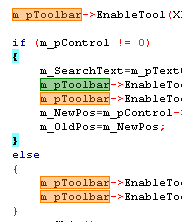
\includegraphics{incremental_search_example}

If the search string cannot be found within the active file, this fact is highlighted by the background of the search mask being displayed in red.

\screenshot{incremental_search_settings}{Settings for Incremental Search}

\begin{description}
\item[ESC] Leave the Incremental Search modus.
\item[ALT-DELETE] Clear the input of the incremental search field.
\end{description}

The icons in the Incremental Search toolbar have the following meanings:

\begin{description}
\item[
\includegraphics{incremental_search_clear}] Deleting the text within the search mask of the Incremental Search toolbar.
\item[
\includegraphics{incremental_search_previous},
\includegraphics{incremental_search_next}] Navigating between the occurrences of a search string.
\item[
\includegraphics{incremental_search_highlight}] Clicking this button results in all the occurrences of the search string within the editor being highlighted in colour, instead of only the initial occurrence.
\item[
\includegraphics{incremental_search_selected}] Activating this option restricts the search to the text passage marked within the editor.
\item[
\includegraphics{incremental_search_matchcase}] This option means a case sensitive search is performed.
\item[
\includegraphics{incremental_search_regex}] Regular expression can be used in the input field of incremental search.
\end{description}

\hint{The standard settings of this toolbar can be configured in \menu{Settings,Editor,Incremental Search}.}

%\screenshot{incremental_search_settings}{Settings for Incremental Search}

\end{INCREMENTALSEARCH}

\begin{NASSISHNEIDERMAN}
\section{NassiShneiderman plugin}\label{sec:nassishneiderman}

NassiShneiderman plugin allows the creation of Nassi Shneiderman diagrams within \codeblocks (\cite{url:nassi}). 

\subsection{Create a diagram}

There are two possibilities to create a diagram.

\begin{enumerate}
\item To create an empty diagram select the menu options \menu{File,New,Nassi Shneiderman diagram}.
\item The second option is to creates a diagram from C/C++ source code. 
\end{enumerate}

In an editor window highlight some code to create the diagram from. For example the body of a function/method from the opening braces till the closing brace. Then right click the selection and choose \menu{Nassi Shneiderman,Create diagram} (see \pxref{fig:NassiShneidermanCreate1}). 

\screenshot{NassiShneidermanCreate1}{NassiShneiderman Create}

You should get a new diagram (see \pxref{fig:NassiShneidermanCreate2}).

\screenshot{NassiShneidermanCreate2}{NassiShneiderman Diagram Example}

The parser has some limitations:

\begin{itemize}
\item Comments can not be at the end of a branch.
\item From a definition of a function it is only able to parse the body, not the declaration.
\item For sure, you will find a lot more... 
\end{itemize}

\subsection{Editing structograms}
\subsubsection{What to do with a diagram?}

You can do a lot of things with a structogram:

\begin{enumerate}
\item Store for later usage. The diagram can be stored \menu{File,Save file} or \menu{File,Save file as...}.
\item It is possible to export to different formats \menu{File,Export}
    \begin{itemize}
    \item "Export source..." to save as C source file.
    \item "StrukTeX" to use in your documentation in LaTeX.
    \item "PNG" or "PS" and eventually "SVG" to have a diagram in an image format known by a lot of other tools.
    \end{itemize}        
\item Directly insert the code into the editor: Open or create a diagram. Back in an editor window right click and choose \menu{Nassi Shneiderman,insert from xy} (You get a list with all open diagrams here).
\item Drag'n'Drop the diagram (or parts of it) to other tools. For example to OpenOffice Writer to get an image in your documentation.
\end{enumerate}

If the chosen diagram has a selection, the export or code-generation takes only this part of the diagram. 

\subsubsection{Extensions}

The NassiShneiderman plugin supports some extensions of Nassi-Shneiderman diagrams: 

\begin{itemize}
\item break has a special brick with an "right-arrow"
\item continue has a special brick with a "left-arrow"
\item To be able to create diagrams from c/c++ switch statements, the selection does not implicitly break before a case. The different cases are vertically aligned. Supports C and C++.
\end{itemize}


\end{NASSISHNEIDERMAN}

\begin{LIBFINDER}
\section{LibFinder}\label{sec:lib_finder}

If you want to use some libraries in your application, you have to configure your project to use them. Such configuration process may be hard and annoying because each library can use custom options scheme. Another problem is that configuration differs on platforms which result in incompatibility between unix and windows projects.

LibFinder provides two major functionalities:

\begin{itemize}
\item Searching for libraries installed on your system
\item Including library in your project with just few mouse clicks making project platform-independent
\end{itemize}

\subsection{Searching for libraries}

Searching for libraries is available under \menu{Plugins,Library finder} menu. It's purpose is to detect libraries installed on your system and store the results inside LibFinder's database (note that these results are not written into \codeblocks project files). Searching starts with dialogue where you can provide set of directories with installed libraries. LibFinder will scan them recursively so if you're not sure you may select some generic directories. You may even enter whole disks -- in such case searching process will take more time but it may detect more libraries (see \pxref{fig:list_of_directories}).

\screenshot{list_of_directories}{List of directories}

When LibFinder scans for libraries, it uses special rules to detect presence of library. Each set of rules is located in xml file. Currently LibFinder can search for wxWidgets 2.6/2.8, \codeblocks SDK and GLFW -- the list will be extended in future.

\hint{To get more details on how to add library support into LibFinder, read \file{src/plugins/contrib/lib\_finder/lib\_finder/readme.txt} in \codeblocks sources.}

After completing the scan, LibFinder shows the results (see \pxref{fig:search_results}).

\screenshot{search_results}{Search results}

In the list you check libraries which should be stored into LibFinder's database. Note that each library may have more than one valid configuration and settings added ealier are more likely to be used while building projects.

Below the list you can select what to do with results of previous scans:

\begin{description}
\item[Do not clear previous results] This option works like an update to existing results -- it adds new ones and updates those which already exist. This option is not recommended.
\item[Second option (Clear previous results for selected libraries)] will clear all results for libraries which are selected before adding new results. This is the recommended option.
\item[Clear all previous library settings] when you select this option, LibFinder's database will be cleared before adding new results. It's useful when you want to clean some invalid LibFinder's database.
\end{description}

Another option in this dialogue is \menu{Set up Global Variables}. When you check this option, LibFinder will try automatically configure Global Variables which are also used to help dealing with libraries.

If you have pkg-config installed on your system (it's installed automatically on most linux versions) LibFinder will also provide libraries from this tool. There is no need to perform scanning for them -- they are automatically loaded when \codeblocks starts.

\subsection{Including libraries in projects}

LibFinder adds extra tab in Project Properties \menu{Libraries} -- this tab shows libs used in project and libs known in LibFinder. To add library into your project, select it in right pane and click $<$ button. To remove library from project, select it on the left pane and click $>$ button (see \pxref{fig:project_configuration}).

\screenshot{project_configuration}{Project configuration}

You can filter libraries known to LibFinder by providing search filter. The \menu{Show as Tree} checkbox allows to switch between categorized and uncategorized view.

If you want to add library which is not available in LibFinder's database, you may use \menu{Unknown Library} field. Note that you should enter library's shortcode (which usually matches global variable name) or name of library in pkg-config. List of suggested shortcodes can be found at \href{http://wiki.codeblocks.org/index.php?title=Recommended_global_variables}{Global Variables}. Using this option is recommended only when preparing project to be built on other machines where such library exists and is properly detected by LibFinder. You can access a global variable within \codeblocks like:

\begin{lstlisting}
$(#GLOBAL_VAR_NAME.include)
\end{lstlisting}

Checking the \menu{Don't setup automatically} option will notify LibFinder that it should not add libraries automatically while compiling this project. In such case, LibFinder can be invoked from build script. Example of such script is generated and added to project by pressing \menu{Add manual build script}.

\subsection{Using LibFinder and projects generated from wizards}

Wizards will create projects that don't use LibFinder. To integrate them with this plugin, you will have to manually update project build options. This can be easily achieved by removing all library-specific settings and adding library through \menu{Libraries} tab in project properties.

Such project becomes cross-platform. As long as used libs are defined in LibFinder's database, project's build options will be automatically updated to match platform-specific library settings.



\end{LIBFINDER}

\begin{SPELLCHECKER}
\section{SpellChecker plugin}\label{sec:spell_checker}

A plugin to check the spelling of strings and comments.

\subsection{Introduction}
A plugin to check the spelling of strings and comments. The spelling gets checked during typing. Additionally a thesaurus is provided. Both may be accessed on-demand by selecting the word in question, then choosing either Spelling... or Thesaurus... from the Edit menu (the operation can be bound to a hot-key via the Keyboard Shortcuts plugin). The context menu (right click the word) provides spelling suggestions. 

\subsection{Configuration}

Configuration is in the menu \menu{Settings,Editor}. The spell check option are about half way down the list on the left.

\screenshot{ConfigureSpellChecker}{SpellChecker Configuration}

The meaning of the controls are: 
\begin{description}
\item[Enable online spell checker] Enable or disable the spell checker.
\item[Language] The language used for spell checking and the thesaurus is selected by choosing a dictionary. This can also be changed in the status bar.
\item[Path settings, Dictionaries] The plugin is looking in this path for the dictionary files.
\item[Path settings, Thesauri] The plugin is looking in this path for the files needed by the thesaurus.
\item[Path settings, Bitmaps] (Optional) The plugin is looking in this path for the flags to show in the status bar.
\end{description}

\hint{You can use Macros in the above three path settings, such as \$(CODEBLOCKS)/share/codeblocks/SpellChecker. See Variable expansion for more details. This is quite convenient if you use portable \codeblocks.}

\subsection{Dictionaries}

SpellChecker uses a library called hunspell. Hunspell is the spell checker of OpenOffice.org, Mozilla Firefox and other projects. Dictionaries available for those applications are compatible with this plugin.

Open Office provides a collection of dictionaries for several languages and dialects to download. The OOo 3.x extensions (*.oxt) are compressed archives which can be opened with your favourite archiver (for example 7-Zip or File Roller). Copy the .aff file and the .dic file to the directory configured in 'Path settings, Dictionaries' (see above).

If you're running Linux you've probably already got compatible dictionaries installed. Look in /usr/share/hunspell or my choice is /usr/share/myspell/dicts. The reason I like the myspell files is they already include thesaurus files which are named correctly to work with the thesaurus, and everything is all in one location. Don't copy these files. Just point the spell checker to where the files are already located.

I understand on Windows, Firefox and Thunderbird also install compatible dictionary files. These can be found in... \file{C:\osp Program Files\osp Mozilla Firefox\osp dictionaries} or \file{C:\osp Program Files\osp Mozilla Thunderbird\osp dictionaries}. In addition, both OpenOffice.org and LibreOffice install dictionary files to\newline
 \file{C:\osp Program Files\osp (Open/Libre)Office\osp share\osp extensions\osp dict-*}.

The Google Chrome browser also installs dictionaries, but they are .bdic format and the \codeblocks spell checker plugin will not work with them.

\subsection{Thesaurus files}

The files for the thesaurus are also available from OOo, like the dictionaries. Copy the thesaurus files (th\_*.dat and th\_*.idx) to the directory configured in 'Path settings, Thesauri' (see above) and rename them to match the name of the dictionary but prepend "th\_" and let the extension as is.

\textbf{Example}: If the dictionary files (for one language) are "en\_GB.aff" and "en\_GB.dic" the files used for the thesaurus are "th\_en\_GB.idx" and "th\_en\_GB.dat".

On my Linux system I found thesaurus files already installed in /usr/share/myspell/dicts and /usr/share/mythes. Again, don't move the files. Set the spell checker to use the files from their current location.

On Windows, if either OpenOffice.org or LibreOffice is installed, they often include thesaurus files in \file{C:\osp Program Files\osp (Open/Libre)Office\osp share\osp extensions\osp dict-*}. 

\subsection{Bitmaps (flags)}

The bitmap of the actually selected language is shown in the status bar. If no bitmap is found, the name of the language is shown. The bitmap must be a PNG image. Choose a flag from the famfamfam\_flag\_icons and copy it to the directory configured in 'Path settings, Bitmaps' (see above) and rename it to match the name of the dictionary but let the extension png.

\subsection{Styles to check}

Only text with specific styles gets checked (for example only comments and strings). Styles are automatically set by Scintilla (CodeBlocks editing component).

The file OnlineSpellChecking.xml contains a list with indices of the styles to check. The indices differ for different programming-languages so the file contains a list for every programming-language. To add styles, look for the name of the programming-language and the indices in the corresponding lexer\_*.xml file and add this information to the file OnlineSpellChecking.xml.

For example, to check the spelling in bash shell scripts (*.sh files), add the line: 

\codeline{<Language name="Bash" index="2,5,6" />}
\end{SPELLCHECKER}

\begin{SRCEXPORTER}
\section{Source Code Exporter}\label{sec:src_exporter}

The necessity occurs frequently of transferring source code to other applications or to e-mails. If the text is simply copied, formatting will be lost, thus rendering the text very unclear.
The \codeblocks export function serves as a remedy for such situations. The required format for the export file can be selected via \menu{File,Export}. The program will then adopt the file name and target directory from the opened source file and propose these for saving the export file. The appropriate file extension in each case will be determined by the export format. The following formats are available.

\begin{description}
\item[html] A text-based format which can be displayed in a web browser or in word processing applications.
\item[rtf] The Rich Text format is a text-based format which can be opened in word processing applications such as Word or OpenOffice.
\item[odt] Open Document Text format is a standardised format which was specified by Sun and O'Reilly. This format can be processed by Word, OpenOffice and other word processing applications.
\item[pdf] The Portable Document Format can be opened by applications such as the Acrobat Reader.
\end{description}

\end{SRCEXPORTER}

\begin{SVN}
\section{SVN Support}\label{sec:svn}

\hint{This extension is now obsolete. So you'll probably no more find it in recent \codeblocks versions.}

The support of the version control system SVN is included in the \codeblocks plugin TortoiseSVN. Via the menu \menu{TortoiseSVN,Plugin settings} you can configure the accessible svn commands in the tab \menu{Integration}.

\begin{description}
\item[Menu integration] Add an entry TortoiseSVN with different settings in the menu bar.
\item[Project manger] Activate the TortoiseSVN commands in the context menu of the project manager.
\item[Editor] Active the TortoiseSVN commands in the context menu of the editor.
\end{description}

In the plugin settings you can configure which svn commands are accessible via the menu or the context menu. The tab integration provides the entry \menu{Edit main menu} and \menu{Edit popup menu} to configure these commands.

\hint{The File Explorer in \codeblocks uses different icon overlays for indicating the svn status. The TortoiseSVN commands are included here in the context menu.}

\end{SVN}

\begin{TODOLIST}
\section{ToDo List}\label{sec:todo_list}

In complex software projects, where different users are involved, there is often the requirement of different tasks to be performed by different users. For this purpose, \codeblocks offers a Todo List. This list can be opened via \menu{View,To-Do list}, and contains the tasks to be performed, together with their priorities, types and the responsible users. The list can be filtered for tasks, users and/or source files. A sorting by columns can be achieved by clicking the caption of the corresponding column.

\screenshot{todo_list}{Displaying the ToDo List}

\hint{The To-Do list can be docked in the message console. Select the option \samp{Include the To-Do list in the message pane} via the menu \menu{Settings,Environment}.}

If the sources are opened in \codeblocks, a Todo can be added to the list via the context menu command \samp{Add To-Do item}. A comment will be added in the selected line of the source code.

\begin{lstlisting}
// TODO (user#1#): add new dialog for next release
\end{lstlisting}

When adding a To-Do, a dialogue box will appear where the following settings can be made (see \pxref{fig:add_todo}).

\figures[hbt!][width=.5\columnwidth]{add_todo}{Dialogue for adding a ToDo}

\begin{description}
\item[User] User name \var{user} in the operating system. Tasks for other users can also be created here. In doing so, the corresponding user name has to be created by Add new. The assignment of a Todo is then made via the selection of entries listed for the User.

\hint{Note that the Users have nothing to do with the Personalities used in \codeblocks.}
\item[Type] By default, type is set to Todo.
\item[Priority] The importance of tasks can be expressed by priorities (1 - 9) in \codeblocks.
\item[Position] This setting specifies whether the comment is to be included before, after or at the exact position of the cursor.
\item[Comment Style] A selection of formats for comments (e.g. doxygen).
\end{description}

\end{TODOLIST}

\begin{TOOLSPLUS}
\section{Tools+}\label{sec:tools+}

Creating a new tool is fairly simple, and can be completed in a few simple steps. First open \menu{Tools(+),Configure Tools...} to access the User-defined Tools dialog.

\screenshot{tools_setup}{User-defined Tools dialog}

\genterm{Tool Name}

This is the name that will be displayed in the Tools(+) drop-down menu. It will also be displayed as the tab name for tools that redirect to the Tools output window.

\genterm{Command Line}

Any valid command line function and switches can be placed here. Variable substitution is also accepted. The following list contains the more useful variables (see \pxref{sec:builtin_variables} for the full list).

\begin{description}
\item[\$relfile, \$file] Respectively, the relative and absolute name of a selected file.
\item[\$reldir, \$dir] Respectively, the relative and absolute name of a selected directory.
\item[\$relpath, \$path] The relative and absolute name of the selected file or directory.
\item[\$mpaths] A list of selected files or directories (absolute paths only).
\item[\$fname, \$fext] The name without extension and the extension without the name of the selected file.
\item[\$inputstr\{prompt\}] Prompts the user to enter a string of text which is substituted into the command line.
\item[\$if(condition)\{true clause\}\{false clause\}] Resolves to \codeline{false clause} if \codeline{condition} is empty, 0, or false; otherwise \codeline{true clause}.
\end{description}

\genterm{File Types}

Wildcard expressions separated by semicolons will restrict population of the right click menu of a file, directory, or multiple paths in the Project Tree, File Explorer, or Editor Pane to the specified type(s). Leave blank to handle all file/directory types.

\genterm{Working Directory}

The directory from which the command is executed. \codeblocks variables, project variables, and global variables are available. Also,

\begin{enumerate}
\item If \codeline{\$dir} is specified in the command line then \codeline{\$dir} may be used here as well.
\item \codeline{\$parentdir} is available for \codeline{\$relfile}, \codeline{\$file}, \codeline{\$reldir}, \codeline{\$dir}, \codeline{\$relpath}, \codeline{\$path}, \codeline{\$fname}, \codeline{\$fext}, evaluating into the absolute path of the directory containing the item.
\end{enumerate}

\genterm{Tools Menu Path}

Controls the placement of the command in the Tools(+) menu, giving the option of adding sub-menus (multiple levels are allowed).

\begin{itemize}
  \item Submenu/Tool1
  \item Submenu/Tool2
  \item Tool3
\end{itemize}

Will create this structure.

\figures[H][width=.6\columnwidth]{tools_menu_path}{Tools menu structure}

The command name will be used if this entry is blank. If the first character is a period, the command will be hidden.

\genterm{Context Menu Path}

This controls the command's placement in the right-click menu of the Projects and Files tabs of the Management pane. The same rules of structure with the Tools Menu Path apply here.

\figures[H][width=.8\columnwidth]{tools_context_path}{Context menu structure}

Please note that the command will not show up in the context menu unless the Command Line contains one or more of the following: \codeline{\$relfile}, \codeline{\$file}, \codeline{\$reldir}, \codeline{\$dir}, \codeline{\$relpath}, \codeline{\$path}, \codeline{\$fname}, and \codeline{\$fext}.

\genterm{Output to}

This determines where the output of the command will be redirected. The purpose and function of the command will determine which is best to select.
\genterm{Tools Output Window}
Tools that only output results command (and require no input) line generally use this setting. The program will be run invisibly and any output will be redirected to the appropriate tab of the Tools Output Window. The text [DONE] will be added upon the tool's completion.

\figures[H][width=.5\columnwidth]{tool_output}{Tool Output window}

\hint{If the Tools Output window is open when \codeblocks is closed, it may trigger \codeblocks to crash.}

\genterm{\codeblocks Console}
This will cause the program to be run through the executable \file{cb\_console\_runner} (the same program that is launched after Build and run). This is generally used for command line tools with more advanced user interactions, although GUI programs can also be used (especially if the program is unstable and/or also leaves messages in the standard output). Console runner will pause the window (prevent it from closing), display the run time, and the exit code when the program finishes.

\genterm{Standard Shell}
This is the same as placing the command in a batch or shell script, then running it. The program will run in whatever its default method is, and when it finishes, its window will close. This setting is useful for running a program (for example a file or web browser) that must remain open after \codeblocks is closed.

\hint{As the Tools+ plugin is not yet complete, some functionality - specifically Menu Priority and Environment Variables - are not available.}

\subsection{Example Tools}

\genterm{Open file browser to selected file}

\begin{itemize}
\item Windows Explorer
\begin{itemize}
\item Tools Menu
\begin{verbatim}
explorer /select,"$(PROJECTFILE)"
\end{verbatim}
\item Context Menu
\begin{verbatim}
explorer /select,"$path"
\end{verbatim}
\end{itemize}

\item Dolphin
\begin{itemize}
\item Tools Menu
\begin{verbatim}
dolphin --select "$(PROJECTFILE)"
\end{verbatim}
\item Context Menu
\begin{verbatim}
dolphin --select "$path"
\end{verbatim}
\end{itemize}

\hint{The following three Context Menu commands only support folders (but not files).}

\item Nautilus
\begin{itemize}
\item Tools Menu
\begin{verbatim}
nautilus --no-desktop --browser "$(PROJECTDIR)"
\end{verbatim}
\item Context Menu
\begin{verbatim}
nautilus --no-desktop --browser "$dir"
\end{verbatim}
\end{itemize}

\item Thunar
\begin{itemize}
\item Tools Menu
\begin{verbatim}
thunar "$(PROJECTDIR)"
\end{verbatim}
\item Context Menu
\begin{verbatim}
thunar "$dir"
\end{verbatim}
\end{itemize}

\item PCMan File Manager
\begin{itemize}
\item Tools Menu
\begin{verbatim}
pcmanfm "$(PROJECTDIR)"
\end{verbatim}
\item Context Menu
\begin{verbatim}
pcmanfm "$dir"
\end{verbatim}
\end{itemize}
\end{itemize}

\genterm{Update Subversion directory}

\begin{itemize}
\item Windows
\begin{itemize}
\item Tools Menu
\begin{verbatim}
"path_to_svn\bin\svn" update "$inputstr{Directory}"
\end{verbatim}
\item Context Menu
\begin{verbatim}
"path_to_svn\bin\svn" update "$dir"
\end{verbatim}
\end{itemize}

\item Linux
\begin{itemize}
\item Tools Menu
\begin{verbatim}
svn update "$inputstr{Directory}"
\end{verbatim}
\item Context Menu
\begin{verbatim}
svn update "$dir"
\end{verbatim}
\end{itemize}
\end{itemize}

\genterm{Export makefile}

\hint{this uses the command line-tool cbp2make.}\label{sec:tool_cbp2make}

\begin{itemize}
\item Windows
\begin{itemize}
\item Tools Menu
\begin{verbatim}
"path_to_cbp2make\cbp2make" -in "$(PROJECTFILE)"
\end{verbatim}
\end{itemize}

\item Linux
\begin{itemize}
\item Tools Menu
\begin{verbatim}
"path_to_cbp2make/cbp2make" -in "$(PROJECTFILE)"
\end{verbatim}
\end{itemize}
\end{itemize}

\genterm{Compress active project to archive}

\begin{itemize}
\item Windows
\begin{itemize}
\item 7z or zip - Tools Menu (on a single line)
\begin{verbatim}
"path_to_7z\7z" a -t$if(zip == $inputstr{7z or zip?}){zip -mm=Deflate
     -mmt=on -mx9 -mfb=128 -mpass=10}{7z -m0=LZMA -mx9 
     -md=64m -mfb=64 -ms=on} -sccUTF-8 "-w$(PROJECTDIR).."
     "$(PROJECTDIR)..\$(PROJECT_NAME)" "$(PROJECTDIR)*"
\end{verbatim}

\item tar.gz or tar.bz2 - Tools Menu (on a single line)
\begin{verbatim}
cmd /c ""path_to_7z\7z" a -ttar -mx0 -sccUTF-8 "-w$(PROJECTDIR).."
      "$(PROJECTDIR)..\$(PROJECT_NAME)" "$(PROJECTDIR)*" && 
      "path_to_7z\7z" a -t$if(gz == $inputstr{gz or bz2?}){gzip -mx9 
      -mfb=128 -mpass=10 -sccUTF-8 "-w$(PROJECTDIR).." 
      "$(PROJECTDIR)..\$(PROJECT_NAME).tar.gz}{bzip2 -mmt=on -mx9 
      -md=900k -mpass=7 -sccUTF-8 "-w$(PROJECTDIR).." 
      "$(PROJECTDIR)..\$(PROJECT_NAME).tar.bz2}"
      "$(PROJECTDIR)..\$(PROJECT_NAME).tar" && 
       cmd /c del "$(PROJECTDIR)..\$(PROJECT_NAME).tar""
\end{verbatim}

\hint{The Windows command line interpreter has been invoked directly here (\cmdline{cmd /c}), allowing for multiple commands to be chained in a single line. However, this causes the command to fail to execute in the \codeblocks Console.}

\end{itemize}

\item Linux
\begin{itemize}
\item 7z or zip - Tools Menu
\begin{verbatim}
7z a -t$if(zip == $inputstr{7z or zip?}){zip -mm=Deflate -mmt=on -mx9
    -mfb=128 -mpass=10}{7z -m0=LZMA -mx9 -md=64m -mfb=64 -ms=on}
    -sccUTF-8 "-w$(PROJECTDIR).." "$(PROJECTDIR)../$(PROJECT_NAME)"
    "$(PROJECTDIR)*"
\end{verbatim}
\item tar.gz or tar.bz2 - Tools Menu
\begin{verbatim}
tar -cf "$(PROJECTDIR)../$(PROJECT_NAME).tar.$if(gz == $inputstr{gz 
     or bz2?}){gz" -I 'gzip}{bz2" -I 'bzip2} -9' "$(PROJECTDIR)*"
\end{verbatim}
\end{itemize}
\end{itemize}

\end{TOOLSPLUS}

\begin{THREADSEARCH}
\section{Thread Search}\label{sec:thread_search}

Via the \menu{Search,Thread Search} menu, the appropriate plug-in can be shown or hidden as a tab in the Messages Console. In \codeblocks, a preview can be displayed for the occurrence of a character string in a file, workspace or directory. In doing so, the list of search results will be displayed on the right-hand side of the ThreadSearch Console. By clicking an entry in the list, a preview is displayed on the left-hand side. By double-clicking in the list, the selected file is opened in the \codeblocks editor.

\hint{The scope of file extensions to be included in the search, is preset and might have to be adjusted.}

\subsection{Features}

ThreadSearch plugin offers the following features:

\begin{itemize}
\item Multi-threaded \samp{Search in files}
\item Internal read-only editor to preview the results
\item File open in editors notebook
\item Highly configurable
\item Contextual menu \samp{Find occurrences} to start a search in files with the word under cursor
\end{itemize}

\screenshot[hbt!][width=1.1\columnwidth]{threadsearch_panel}{Thread Search Panel}

\subsection{Usage}

\begin{enumerate}
\item Configure your search preferences (see \pxref{fig:threadsearch_options})

Once the plugin is installed, there are 4 ways to run a search:

\begin{enumerate}
\item Type/Select a word in the search combo box and press enter or click on Search on the Thread search panel of the Messages notebook.
\item Type/Select a word in the toolbar search combo box and press enter or click on Search button.
\item Right click on any \samp{word} in active editor and click on \samp{Find occurrences}.
\item Click on Search/Thread search to find the current word in active editor.
\hint{Items 1, 2 and 3 may not be available according to current configuration.}
\end{enumerate}
\item Click again on the search button to cancel current search.
\item A single click on a result item displays it on the preview editor at right location.
\item A double click on a result item opens or set an editor in editors notebook at right location.
\end{enumerate}

\subsection{Configuration}

To access ThreadSearch plugin configuration panel click on (see \pxref{fig:threadsearch_options}):

\screenshot{threadsearch_options}{Configuration of Thread Search}

\begin{enumerate}
\item Options button on Messages notebook Thread search panel.
\item Options button on Thread search toolbar.
\item Settings/Environment menu item and then on the Thread search item on the left columns.
\end{enumerate}

\hint{Items 1, 2 and 3 may not be available according to current configuration.}

Search in part defines the set of files that will be analysed.

\begin{itemize}
\item Project and Workspace checkboxes are mutually exclusive.
\item Directory path can be edited or set with Select button.
\item Mask is the set a file specifications separated by \samp{;}. For example: \file{*.cpp;*.c;*.h.}
\end{itemize}

\subsection{Options}

\begin{description}
\item[Whole word] if checked, line matches search expression if search expression is found with no alpha-numeric \codeline{+'_'} before and after.
\item[Start word] if checked, line matches search expression if search expression is found at the beginning of a word, ie no alpha-numeric \codeline{+'_'} before search expression.
\item[Match case] if checked, the search is case sensitive.
\item[Regular expression] the search expression is a regular expression.
\end{description}

\hint{If you want to search for regular expressions like \codeline{\n} you will have to set the option \menu{Use Advanced RegEx searches} via the menu \menu{Settings,Editor,General Settings}.}

\subsection{Thread search options}

\begin{description}
\item[Enable \samp{Find occurrences contextual menu item}] If checked, the Find occurrences of \samp{Focused word} entry is added to the editor contextual menu.
\item[Use default options when running \samp{Find occurrences}] If checked, a set of default options is applied to the searches launched with the \samp{Find occurrences} contextual menu item. Per defaut option \samp{Whole word} and \samp{Match case} is enabled.
\item[Delete previous results at search begin] If ThreadSearch is configured with \samp{Tree View} then the search results will be listed hierarchically,
\begin{itemize}
\item the first node contains the search term
\item above the files which contain the search term are listed
\item within this list the line number and the corresponding content of the occurence is displayed
\end{itemize}
If you search different terms the list will become confusing, therefore previous search results can be cleared at search begin using this option.
\hint{In the list of occurences single items or all items can be deleted via the context menu \menu{Delete item} or \menu{Delete all items}.}
\end{description}

\subsection{Layout}

\begin{description}
\item[Display header in log window] if checked, the header are displayed in the results list control.
\hint{If unchecked, the columns are no longer resizeable but space is spared.}
\item[Draw lines between columns] Draws lines between columns in list mode.
\item[Show ThreadSearch toolbar] Display the toolbar of Thread Search plugin.
\item[Show search widgets in ThreadSearch Messages panel] If checked, only the results list control and the preview editor are displayed. All other search widgets are hidden (spares space).
\item[Show code preview editor] Code preview can be hidden either with this check box or with a double click on the splitter window middle border. This is where it can be shown again.
\end{description}

\subsection{Panel Management}

You can choose different modes how the the ThreadSearch window is managed. With the setting \samp{Message Notebook} the ThreadSearch window will be a dockable window in the message panel. If you choose the setting \samp{Layout} you will be able to undock the window from the message panel and put it somewhere else.

\subsection{Logger Type}

The view of the search results can be displayed in different ways. The setting \samp{List} displays all occurrences as list. The other mode \samp{Tree} gathers all occurrences within a file as a node.

\subsection{Splitter Window Mode}

The user can configure a horizontal or vertical splitting of the preview window and the output window of the search results.

\subsection{Sort Search Results}

The view of the search results may be sorted by path or file name.

\end{THREADSEARCH}

\begin{MOREPLUGINS}
\section{Code statistics}

\screenshot{code_stats}{Configuration for Code Statistics}

Based on the entries in the configuration mask, this simple plugin detects the proportions of code, commentaries and blank lines for a project. The evaluation is called via the menu command \menu{Plugins,Code statistics}.


\section{Code profiler}

A simple graphical interface to the GNU GProf Profiler.


\section{Projects Importer plugin}

ProjectsImporter imports foreign projects and workspaces from Dev-C++, MSVC6, MSVC7, and MSVC8 for use as a \codeblocks project. 


\section{Searching Available Source Code}

This plugin makes it possible to select a term within the editor and to search for this term via the context menu \menu{Search at Koders} in the \cite{url:koders} database. The dialog offers the additional possibilities to of filtering for program languages and licences.

\hint{Koders and it's successor BlackDuck seem to have disappeared or changed their website ! So this plugin does not work anymore. Waiting for an update ...}

This database search will help you find source code originating from other world-wide projects of universities, consortiums and organisations such as Apache, Mozilla, Novell Forge, SourceForge and many others, which can be re-used without having to reinvent the wheel every time. Please observe the licence of the source code in each individual case.


\section{Symbol Table Plugin}

This plugin makes it possible to search for symbols in objects and libraries. The options and the path for the command line program nm are defined in the Options tab.

\screenshot{symtab_config}{Configuring the Symbol Table}

Clicking the \samp{Search} stats the search, the results of the NM program are displayed in a separate window caleld \samp{SymTabs Result}. The name of the objects or libraries containing the symbol are listed under the title \samp{NM's Output}.


\end{MOREPLUGINS}

%\section{Code statistics}

\screenshot{code_stats}{Configuration for Code Statistics}

Based on the entries in the configuration mask, this simple plugin detects the proportions of code, commentaries and blank lines for a project. The evaluation is called via the menu command \menu{Plugins,Code statistics}.


\section{Code profiler}

A simple graphical interface to the GNU GProf Profiler.


\section{Projects Importer plugin}

ProjectsImporter imports foreign projects and workspaces from Dev-C++, MSVC6, MSVC7, and MSVC8 for use as a \codeblocks project. 


\section{Searching Available Source Code}

This plugin makes it possible to select a term within the editor and to search for this term via the context menu \menu{Search at Koders} in the \cite{url:koders} database. The dialog offers the additional possibilities to of filtering for program languages and licences.

\hint{Koders and it's successor BlackDuck seem to have disappeared or changed their website ! So this plugin does not work anymore. Waiting for an update ...}

This database search will help you find source code originating from other world-wide projects of universities, consortiums and organisations such as Apache, Mozilla, Novell Forge, SourceForge and many others, which can be re-used without having to reinvent the wheel every time. Please observe the licence of the source code in each individual case.


\section{Symbol Table Plugin}

This plugin makes it possible to search for symbols in objects and libraries. The options and the path for the command line program nm are defined in the Options tab.

\screenshot{symtab_config}{Configuring the Symbol Table}

Clicking the \samp{Search} stats the search, the results of the NM program are displayed in a separate window caleld \samp{SymTabs Result}. The name of the objects or libraries containing the symbol are listed under the title \samp{NM's Output}.

      % already called in plugins_en
\chapter{Variable Expansion}\label{sec:variables_types}

\codeblocks differentiates between several types of variables. These types serve the purpose of configuring the environment for creating a program, and at the same of improving the maintainability and portability. Access to the \codeblocks variables is achieved via \codeline{$<name>}.


\begin{description}
\item[Environment Variable] are set during the startup of \codeblocks. They can modify system environment variables such as \codeline{PATH}. This can be useful in cases where a defined environment is necessary for the creation of projects. The settings for environment variables in \codeblocks are made at \menu{Settings,Environment,Environment Variables}.
\item[Builtin Variables] are predefined in \codeblocks, and can be accessed via their names  (see \pxref{sec:builtin_variables} for details).
\item[Command Macros] This type of variables is used for controlling the build process. For further information please refer to \pxref{sec:command_macros}.
\item[Custom Variables] are user-defined variables which can be specified in the build options of a project. Here you can, for example define your derivative as a variable \codeline{MCU} and assign a corresponding value to it. Then set the compiler option \opt{-mcpu=\$(MCU)}, and \codeblocks will automatically replace the content. By this method, the settings for a project can be further parametrised.
\item[Global Variables] are mainly used for creating \codeblocks from the sources or developments of wxWidgets applications. These variables have a very special meaning. In contrast to all others if you setup such a variables and share your project file with others that have *not* setup this GV \codeblocks will ask the user to setup the variable. This is a very easy way to ensure the \samp{other developer} knows what to setup easily. \codeblocks will ask for all path's usually necessary.
\end{description}

\section{Syntax}

\codeblocks treats the following functionally identical character sequences inside pre-build, post-build, or build steps as variables:

\begin{itemize}
\item \codeline{$VARIABLE}
\item \codeline{$(VARIABLE)}
\item \codeline{$\{VARIABLE\}}
\item \codeline{\%VARIABLE\%}
\end{itemize}

Variable names must consist of alphanumeric characters and are not case-sensitive. Variables starting with a single hash sign \codeline{(#)} are interpreted as global user variables (see \pxref{sec:global_variables} for details). The names listed below are interpreted as built-in types.

Variables which are neither global user variables nor built-in types, will be replaced with a value provided in the project file, or with an environment variable if the latter should fail.

The use of these variables can follow the following example for the date :

\codeline{#include "include/manager.h"} \newline
\codeline{wxString strdate = Manager::Get()->GetMacrosManager()->ReplaceMacros(_T("$TODAY"));}

\hint{Per-target definitions have precedence over per-project definitions.}

\section{List of available built-ins}\label{sec:builtin_variables}

The variables listed here are built-in variables of \codeblocks. They cannot be used within source files.

\subsection{\codeblocks workspace}

\begin{description}
\item[{\scriptsize \$(WORKSPACE\_FILENAME), \$(WORKSPACE\_FILE\_NAME), \$(WORKSPACEFILE), \$(WORKSPACEFILENAME)}] The filename of the current workspace project (.workspace).
\item[{\scriptsize \$(WORKSPACENAME), \$(WORKSPACE\_NAME)}] The name of the workspace that is displayed in tab Projects of the Management panel.
\item[{\scriptsize \$(WORKSPACE\_DIR), \$(WORKSPACE\_DIRECTORY), \$(WORKSPACEDIR), \$(WORKSPACEDIRECTORY)}] The location of the workspace directory.
\end{description}

\subsection{Files and directories}

\begin{description}
\item[{\footnotesize \$(PROJECT\_FILENAME), \$(PROJECT\_FILE\_NAME), \$(PROJECT\_FILE), \$(PROJECTFILE)}] The filename of the currently compiled project.
\item[{\footnotesize \$(PROJECT\_NAME), \$(PROJECTNAME)}] The name of the currently compiled project.
\item[{\footnotesize \$(PROJECT\_DIR), \$(PROJECTDIR), \$(PROJECT\_DIRECTORY), \$(PROJECTDIRECTORY)}] The common top-level directory of the currently compiled project.
\item[{\footnotesize \$(ACTIVE\_EDITOR\_FILENAME)}] The filename of the file opened in the currently active editor.
\item[{\footnotesize \$(ACTIVE\_EDITOR\_LINE)}] Return the current line in the active editor.
\item[{\footnotesize \$(ACTIVE\_EDITOR\_COLUMN}] Return the column of the current line in the active editor.
\item[{\footnotesize \$(ACTIVE\_EDITOR\_DIRNAME)}] the directory containing the currently active file (relative to the common top level path).
\item[{\footnotesize \$(ACTIVE\_EDITOR\_STEM)}] The base name (without extension) of the currently active file.
\item[{\footnotesize \$(ACTIVE\_EDITOR\_EXT)}] The extension of the currently active file.
\item[{\footnotesize \$(ALL\_PROJECT\_FILES)}] A string containing the names of all files in the current project.
\item[{\footnotesize \$(MAKEFILE)}] The filename of the makefile.
\item[{\footnotesize \$(CODEBLOCKS), \$(APP\_PATH), \$(APPPATH), \$(APP-PATH)}] The path to the currently running instance of \codeblocks.
\item[{\footnotesize \$(DATAPATH), \$(DATA\_PATH), \$(DATA-PATH)}] The 'shared' directory of the currently running instance of \codeblocks.
\item[{\footnotesize \$(PLUGINS)}] The \file{plugins} directory of the currently running instance of \codeblocks.
\item[{\footnotesize \$(TARGET\_COMPILER\_DIR)}] The compiler installation directory so-called master path.
\end{description}

\subsection{Build targets}

replace FOOBAR with the target name 

\begin{description}
\item[{\footnotesize \$(FOOBAR\_OUTPUT\_FILE)}] The output file of a specific target.
\item[{\footnotesize \$(FOOBAR\_OUTPUT\_DIR)}] The output directory of a specific target.
\item[{\footnotesize \$(FOOBAR\_OUTPUT\_BASENAME)}] The output file's base name (no path, no extension) of a specific target.
\item[{\footnotesize \$(FOOBAR\_PARAMETERS)}] A specific target's execution parameters
\item[{\footnotesize \$(TARGET\_OUTPUT\_DIR)}] The output directory of the current target.
\item[{\footnotesize \$(TARGET\_OBJECT\_DIR)}] The object directory of the current target.
\item[{\footnotesize \$(TARGET\_NAME)}] The name of the current target.
\item[{\footnotesize \$(TARGET\_OUTPUT\_FILE)}] The output file of the current target.
\item[{\footnotesize \$(TARGET\_OUTPUT\_BASENAME)}] The output file's base name (no path, no extension) of the current target.
\item[{\footnotesize \$(TARGET\_CC), \$(TARGET\_CPP), \$(TARGET\_LD), \$(TARGET\_LIB)}] The build tool executable (compiler, linker, etc) of the current target.
\item[{\footnotesize \$(TARGET\_COMPILER\_DIR)}] The current target's build tool directory (compiler, linker, etc).
\end{description}

\subsection{Language and encoding}

\begin{description}
\item[{\footnotesize \$(LANGUAGE)}] The system language in plain language.
\item[{\footnotesize \$(ENCODING)}] The character encoding in plain language.
\end{description}

\subsection{Time and date}

\begin{description}
\item[{\footnotesize \$(TDAY)}] Current date in the form YYYYMMDD (for example 20051228)
\item[{\footnotesize \$(TODAY)}] Current date in the form YYYY-MM-DD (for example 2005-12-28)
\item[{\footnotesize \$(NOW)}] Timestamp in the form YYYY-MM-DD-hh.mm (for example 2005-12-28-07.15)
\item[{\footnotesize \$(NOW\_L)}] Timestamp in the form YYYY-MM-DD-hh.mm.ss (for example 2005-12-28-07.15.45)
\item[{\footnotesize \$(WEEKDAY)}]  Plain language day of the week (for example \samp{Wednesday})
\item[{\footnotesize \$(TDAY\_UTC), \$(TODAY\_UTC), \$(NOW\_UTC), \$(NOW\_L\_UTC), \$(WEEKDAY\_UTC)}] These are identical to the preceding types, but are expressed relative to UTC.
\item[{\footnotesize \$(DAYCOUNT)}] The number of the days passed since an arbitrarily chosen day zero (January 1, 2009). Useful as last component of a version/build number.
\end{description}

\subsection{Platform dependence}

\begin{description}
\item[{\footnotesize \$(PLATFORM)}] Expands to msw on windows and unix on linux and mac (Since revision r11793) 
\end{description}

\subsection{Command line expansions}
This commands can be used in the command line for the specific platform. 
\begin{description}
\item[{\footnotesize \$(CMD\_CP)}] Will expand to a copy command for the specific platform. (on windows \codeline{copy} and on unix \codeline{cp --preserve=timestamps}) 
\item[{\footnotesize \$(CMD\_RM)}] delete command
\item[{\footnotesize \$(CMD\_MV)}] move command
\item[{\footnotesize \$(CMD\_NULL)}] NULL device (for redirecting streams)
\item[{\footnotesize \$(CMD\_MKDIR)}] create a directory
\item[{\footnotesize \$(CMD\_RMDIR)}] delete a directory
\end{description}

\subsection{Random values}

\begin{description}
\item[{\footnotesize \$(COIN)}] This variable tosses a virtual coin (once per invocation) and returns 0 or 1.
\item[{\footnotesize \$(RANDOM)}] A 16-bit positive random number (0-65535)
\end{description}

\subsection{Standard path}

\begin{description}
\item[{\footnotesize \$(GET\_DATA\_DIR)}] Unix: prefix/share/appname ; Windows: EXE path
\item[{\footnotesize \$(GET\_LOCAL\_DATA\_DIR)}] Unix: /etc/appname ; Windows: EXE path
\item[{\footnotesize \$(GET\_CONFIG\_DIR)}] Unix: /etc ; Windows: \file{C:\osp Documents and Settings\osp All Users\osp Application Data}
\item[{\footnotesize \$(GET\_USER\_CONFIG\_DIR)}] Unix: ~ ; Windows: \file{C:\osp Documents and Settings\osp username\osp Application Data\osp appname}
\item[{\footnotesize \$(GET\_USER\_DATA\_DIR)}] Unix: ~/.appname ; Windows: \file{C:\osp Documents and Settings\osp username\osp Application Data}
\item[{\footnotesize \$(GET\_USER\_LOCAL\_DATA\_DIR)}] Unix: ~/.appname ; Windows: \file{C:\osp Documents and Settings\osp username\osp Local Settings\osp Application Data\osp appname}
\item[{\footnotesize \$(GET\_TEMP\_DIR)}] ALL platforms: A writable, temporary directory
\end{description}

\subsection{Build in functions for path conversion}
There are build in macro functions to simplify path generation 
\begin{description}
\item[{\footnotesize \$TO\_UNIX\_PATH\{\}}] convert path to unix path (use '/' as separator)
\item[{\footnotesize \$TO\_WINDOWS\_PATH\{\}}] convert path to windows (use '\osp' as separator)
\item[{\footnotesize \$TO\_NATIVE\_PATH\{\}}] convert to native path form the codeblocks instance is running on
\end{description}

\textbf{Usage}
\begin{description}
\item[{\footnotesize \$TO\_UNIX\_PATH\{\$(TARGET\_OUTPUT\_FILE)\}}] returns the current target output file as unix path
\end{description}

\subsection{Conditional Evaluation}

\begin{lstlisting}
$if(condition){true clause}{false clause}
\end{lstlisting}

Conditional evaluation will resolve to its true clause if

\begin{itemize}
\item condition is a non-empty character sequence other than 0 or false
\item condition is a non-empty variable that does not resolve to 0 or false
\item condition is a variable that evaluates to true (implicit by previous condition)
\end{itemize}

Conditional evaluation will resolve to its false clause if

\begin{itemize}
\item condition is empty
\item condition is 0 or false
\item condition is a variable that is empty or evaluates to 0 or false
\end{itemize}

\hint{Please do note that neither the variable syntax variants \codeline{\%if(...)} nor \codeline{\$(if)(...)} are supported for this construct.}

\genterm{Example}

For example if you are using several platforms and you want to set different parameters depending on the operating system. In the following code the script commands of \codeline{[[ ]]} are evaluated and the \var{command} will be executed. This could be useful in a post-built step (on a single line).

\begin{lstlisting}
[[ if (PLATFORM ==  PLATFORM_MSW) { print (_T("cmd /c")); } else
      { print (_T("sh ")); } ]] <command>
\end{lstlisting}

\section{Script expansion}

For maximum flexibility, you can embed scripts using the \codeline{[[ ]]} operator as a special case of variable expansion. Embedded scripts have access to all standard functionalities available to scripts and work pretty much like bash backticks (except for having access to \codeblocks namespace). As such, scripts are not limited to producing text output, but can also manipulate \codeblocks state (projects, targets, etc.).

\hint{Manipulating \codeblocks state should be implemented rather with a pre-build script than with a script.}

\genterm{Example with Backticks}

\begin{lstlisting}
objdump -D `find . -name *.elf` > name.dis
\end{lstlisting}

The expression in backticks returns a list of all executables \file{*.elf} in any subdirectories. The result of this expression can be used directly by \cmdline{objdump}. Finally the output is piped to a file named  \file{name.dis}. Thus, processes can be automatted in a simple way without having to program any loops.

\genterm{Example using Script}

The script text is replaced by any output generated by your script, or discarded in case of a syntax error.

Since conditional evaluation runs prior to expanding scripts, conditional evaluation can be used for preprocessor functionalities. Built-in variables (and user variables) are expanded after scripts, so it is possible to reference variables in the output of a script.

\begin{lstlisting}
[[ print(GetProjectManager().GetActiveProject().GetTitle()); ]]
\end{lstlisting}

inserts the title of the active project into the command line.

\section{Command Macros}\label{sec:command_macros}

\begin{description}
\item[\$compiler] Access to name of the compiler executable.
\item[\$linker] Access to name of the linker executable.
\item[\$options] Compiler flags
\item[\$link\_options] Linker flags
\item[\$includes] Compiler include paths
\item[\$c] Linker include paths
\item[\$libs] Linker libraries
\item[\$file] Source file (full name)
\item[\$file\_dir] Source file directory without file name and file name extension.
\item[\$file\_name] Source file name without path info and file name extension.
\item[\$exe\_dir] Directory of executable without file name and file name extension.
\item[\$exe\_name] File name of executable without path and file name extension.
\item[\$exe\_ext] File name extension of executable without path and file name.
\item[\$object] Object file
\item[\$exe\_output] Executable output file
\item[\$objects\_output\_dir] Object Output Directory
\end{description}

\subsection{Example 1: Compile single file}

\begin{lstlisting}
$compiler $options $includes -c $file -o $object
\end{lstlisting}

\subsection{Example 2: Link object files to executable}

\begin{lstlisting}
$linker $libdirs -o $exe_output $link_objects $link_resobjects 
$link_options $libs
\end{lstlisting}

\section{Global compiler variables}\label{sec:global_variables}

This section describes how to work with global variables.

\subsection{Synopsis}

Working as a developer on a project which relies on 3rd party libraries involves a lot of unnecessary repetitive tasks, such as setting up build variables according to the local file system layout. In the case of project files, care must be taken to not accidentially commit a locally modified copy. If one does not pay attention, this can happen easily for example after changing a build flag to make a release build.

The concept of global compiler variables is a unique new solution for \codeblocks which addresses this problem. Global compiler variables allow you to set up a project once, and any number of developers using any number of different file system layouts being able to compile and develop this project. No local layout information ever needs to be changed more than once.

\subsection{Names and Members}

Global compiler variables in \codeblocks are discriminated from per-project variables by a leading hash sign. Global compiler variables are structured; every variable consists of a name and an optional member. Names are freely definable, while some of the members are built into the IDE. Although you can choose anything for a variable name in principle, it is advisable to pick a known identifier for common packages. Thus the amount of information that the user needs to provide is minimised. The \codeblocks team provides a list of recommended variables for known packages.

The member base resolves to the same value as the variable name uses without a member (alias).

The members \codeline{include} and \codeline{lib} are by default aliases for \codeline{base/include} and \codeline{base/lib}, respectively. However, a user can redefine them if another setup is desired.

It is generally recommended to use the syntax \codeline{$(#variable.include)} instead of \codeline{$(#variable)/include}, as it provides additional flexibility and is otherwise exactly identical in functionality (see \pxref{sec:mini_tutorial} and \pxref{fig:gcv_ui} for details).

The members \codeline{cflags} and \codeline{lflags} are empty by default and can be used to provide the ability to feed the same consistent set of compiler/linker flags to all builds on one machine. \codeblocks allows you to define custom variable members in addition to the built-in ones.

\figures[H][width=.8\columnwidth]{gcv_ui}{Global Variable Environment}
\subsection{Constraints}

\begin{itemize}
\item Both set and global compiler variable names may not be empty, they must not contain white space, must start with a letter and must consist of alphanumeric characters. Cyrillic or Chinese letters are not alphanumeric characters. If \codeblocks is given invalid character sequences as names, it might replace them without asking.
\item Every variable requires its base to be defined. Everything else is optional, but the base is absolutely mandatory. If you don't define a the base of a variable, it will not be saved (no matter what other fields you have defined).
\item You may not define a custom member that has the same name as a built-in member. Currently, the custom member will overwrite the built-in member, but in general, the behaviour for this case is undefined. If \codeline{'libext'} is a custom member we can only write \codeline{$(#variable.libext)} and not \codeline{$(#variable)/libext}.
\item Variable and member values may contain arbitrary character sequences, subject to the following three constraints:
\begin{itemize}
\item You may not define a variable by a value that references the same variable or any of its members
\item You may not define a member by a value that references the same member
\item You may not define a member or variable by a value that references the same variable or member through a cyclic dependency.
\end{itemize}
\end{itemize}

\codeblocks will detect the most obvious cases of recursive definitions (which may happen by accident), but it will not perform an in-depth analysis of every possible abuse. If you enter crap, then crap is what you will get; you are warned now.

\genterm{Examples}

Defining \codeline{wx.include} as \codeline{$(#wx)/include} is redundant, but perfectly legal
Defining \codeline{wx.include} as \codeline{$(#wx.include)} is illegal and will be detected by \codeblocks
Defining \codeline{wx.include} as \codeline{$(#cb.lib)} which again is defined as \codeline{$(#wx.include)} will create an infinite loop

\subsection{Using Global Compiler Variables}

All you need to do for using global compiler variables is to put them in your project! Yes, it's that easy.

When the IDE detects the presence of an unknown global variable, it will prompt you to enter its value. The value will be saved in your settings, so you never need to enter the information twice.

If you need to modify or delete a variable at a later time, you can do so from the settings menu.


\genterm{Example}

\screenshot{global_vars_dir}{Global Variables}

The above image shows both per-project and global variables. \codeline{WX_SUFFIX} is defined in the project, but \codeline{WX} is a global user variable.

\subsection{Variable Sets}

Sometimes, you want to use different versions of the same library, or you develop two branches of the same program. Although it is possible to get along with a global compiler variable, this can become tedious. For such a purpose, \codeblocks supports variable sets. A variable set is an independent collection of variables identified by a name (set names have the same constraints as variable names).

If you wish to switch to a different set of variables, you simply select a different set from the menu. Different sets are not required to have the same variables, and identical variables in different sets are not required to have the same values, or even the same custom members.

Another positive thing about sets is that if you have a dozen variables and you want to have a new set with one of these variables pointing to a different location, you are not required to re-enter all the data again. You can simply create a clone of your current set, which will then duplicate all of your variables.

Deleting a set also deletes all variables in that set (but not in another set). The \file{default} set is always present and cannot be deleted.

You can also export or import sets: files, with extension .set, are text files containing a particular set. Those files are easily transferable between users/computers.

All these options on sets are available with buttons "Add", "Delete", "Clone", "Export" and "Import", located at the top of the Global Variable Environment window (see \pxref{fig:gcv_ui}).

\subsection{Custom Members Mini-Tutorial}\label{sec:mini_tutorial}

As stated above, writing \codeline{$(#var.include)} and \codeline{$(#var)/include} is exactly the same thing by default. So why would you want to write something as unintuitive as \codeline{$(#var.include)}?

Let's take a standard Boost installation under Windows for an example. Generally, you would expect a fictional package ACME to have its include files under ACME/include and its libraries under ACME/lib. Optionally, it might place its headers into yet another subfolder called acme. So after adding the correct paths to the compiler and linker options, you would expect to \codeline{\#include <acme/acme.h>} and link to \file{libacme.a} (or whatever it happens to be).

Boost, however, installs headers into \file{C:\osp Boost\osp include\osp boost-1\_33\_1\osp boost} and its libraries under \file{C:\osp Boost\osp lib} by default. It seems impossible to get this under one hood without having to adjust everything on every new PC, especially if you have to work under Linux or some other OS, too.

This is where the true power of global user variables is unveiled. When defining the value of the \codeline{#boost} variable, you go one step further than usual. You define the member include as \file{C:\osp Boost\osp include\osp boost-1\_33\_1\osp boost} and the member lib as \file{C:\osp Boost\osp lib}, respectively. Your projects using \codeline{$(#boost.include)} and \codeline{$(#boost.lib)} will magically work on every PC without any modifications. You don't need to know why, you don't want to know why.

\subsection{Command line arguments}\label{sec:cmdline_args}
After revision [r13245] it is possible to use command line arguments to override and define global variables and set the current active set.
\begin{itemize}
\item '-S' parameter for setting current active set via command line
\item '-D' parameter for defining/overriding user variable in form:\\
 \codeline{-D set.variable.member=value} or \codeline{-D variable.member=value}
\end{itemize}
\chapter{Working With \codeblocks}

This chapter deals with some basic knowledge to be able to work with \codeblocks. Some paragraphs, here directly taken from Wiki, overlap but with a slightly different presentation with the content of the first chapter.

\begin{BUILDPROCESS}
\section{The build process of \codeblocks}\label{sec:build_process}

In this pages, the build process is explained in detail. What goes on behind the scenes and "when" is covered. I hope it makes an interesting read :).
 
\subsection{Build order}

As you have probably guessed, \codeblocks does not launch build commands at random but rather as a well thought out and prepared sequence. But first let's see what components are the subject of the build:

\begin{description}
\item[Workspace:] contains one or more projects
\item[Project:] contains one or more build targets. It also contains the project's files.
\item[Build target:] project files are assigned to it, which are built as a group and generate one binary output. This output can either be an executable, a dynamic library or a static library. NOTE: there is one kind of build target that does not produce a binary output directly but rather just runs its pre/post build steps (which may generate a binary output externally).
\end{description}

Let's break these subjects in sections and explain them in more detail.

\subsection{Workspace}

The workspace is the top-level container item for organizing your projects. Since there can be only one workspace open at a time, there really is no build order issue for them. It's only one, so it's just built ;).

Use the menu \menu{Build,Build workspace} to build a workspace (i.e. all the projects contained in it). 

\subsection{Projects}

Here, things start getting interesting :).

Projects build order is different depending if the user has set project dependencies or not. Please read on.

\genterm{Without project dependencies}

In this case, projects are built in the order of appearence, from top to bottom. Most projects though (at least not the "hello world" ones), would want to setup project dependencies.

\genterm{Using project dependencies}

Project dependencies are a simple way to tell \codeblocks that a given project "depends" on another (in the same workspace, always).

Thus imagine in your workspace you have a library project and an executable project which depends on the library. Then you could (and should) tell \codeblocks about this dependency. To do this, you select \menu{Project,Properties} and click the "Project's dependencies.." button.

\textit{Please notice that the dependency information is saved within the workspace file, not the project file as it is a dependency between two projects within a workspace.}

\figures[H][width=.55\columnwidth]{Project_deps}{Setting up project dependencies}

It is very easy to use this dialog. Select the project you want to add a dependency and then put a checkmark on all projects that this project depends on. This will ensure that all the projects you checked will be built before the project that depends on them, ensuring a synchronized build.

\textbf{Tip:} You don't have to close this dialog and launch the other project's properties again to set their dependencies. You can set all projects dependencies from this same dialog. Just select a different project in the drop-down box :).

Some things to note:

\begin{itemize}
\item Dependencies are set directly or indirectly. If project A depends directly on project B and project B depends on project C, then project A indirectly depends on project C too.
\item \codeblocks is smart enough to watch out for circular dependencies and prohibit them. A circular dependency is caused when project A depends directly or indirectly on project B and project B depends directly or indirectly on project A.
\item Dependencies take effect either if building the whole workspace or a single project. In this case, only the dependencies needed for the project you 're building will be built too.
\end{itemize}

\subsection{Build targets}

Build targets build order depend on a couple of things.

\begin{enumerate}
\item If the user has selected a specific build target in the compiler toolbar's drop-down box, then only this build target is built. If project dependencies are setup for the project containing this target, all projects it depends on will also build their target with the same name. If no such target exists, that project is skipped.
\item If the virtual "All" target is selected, then all targets in the project (and all the projects it depends on) are built in order, top to bottom. There are a couple of exceptions to this:
    \begin{itemize}
    \item A target is not built with "All" if the target option (in project properties "Targets" page) "Build this target with All" is not selected.
    \item If no targets in the project have the above option selected, then no virtual "All" target appears in the list.
    \end{itemize}
\end{enumerate}

\subsection{Preprocessing phase}

Before the actual build process starts (i.e. the compiler/linker commands start executing), a preprocessing step runs which generates all required command-lines for the entire build process. This step caches much of the information it generates, making subsequent builds faster in effect.

This step also runs any attached build scripts.


\subsection{Actual commands execution}

This is the stage that the build process actually starts, from the user's point of view. The files start getting compiled and finally linked to generate the various binary outputs the build targets define.

In this step, the pre-build and post-build steps are also executed.


\subsection{Pre-build and post-build steps}

These are commands that can be setup on project and/or target level. They are shell commands that e.g. copy files around or any other operation you can do with a usual OS system shell.

The variables specified in the article Variable expansion (\pxref{sec:variables_types}) can be used in the scripts to get things like target output directory, project directory, target type and others.

Here's a breakdown of the pre/post build steps execution order for an imaginary project with two targets (Debug/Release):

\begin{enumerate}
\item Project pre-build steps
    \begin{enumerate}
    \item Target "Debug" pre-build steps
    \item Target "Debug" compile files
    \item Target "Debug" link files and generate binary output
    \item Target "Debug" post-build steps (see notes below)
    \item Target "Release" pre-build steps
    \item Target "Release" compile files
    \item Target "Release" link files and generate binary output
    \item Target "Release" post-build steps (see notes below)
    \end{enumerate}
\item Project post-build steps
\end{enumerate}

I hope this is self-explaining :)

\hint{Pre-build steps are always ran. Post-build steps will run only if the project/target they 're attached to is not up-to-date (i.e. is going to be built). You can change this by selecting "Always execute, even if target is up to date" in the build options.}

\genterm{Script Samples}

Post-build script that copies the output file into the folder \file{C:\osp Program\osp bin} in Windows: 

\begin{lstlisting}
cmd /c copy "$(PROJECT_DIR)$(TARGET_OUTPUT_FILE)" "C:\Program\bin"
\end{lstlisting}

Execute the bash script "copyresources.sh" in Linux:

\begin{lstlisting}
/bin/sh copyresources.sh
\end{lstlisting}

Create a new directory in the output directory:

\begin{lstlisting}
mkdir $(TARGET_OUTPUT_DIR)/data
\end{lstlisting}  

\end{BUILDPROCESS}

\begin{CREATEPROJECT}
\section{Creating a New Project}\label{sec:create_project}

These pages are a guide to many of the beginning (and some intermediate) features of the creation and modification of a \codeblocks project. If this is your first experience with \codeblocks, here is a good starting point. 
 
\subsection{The project wizard}

Launch the Project Wizard through \menu{File,New,Project...} to start a new project. Here there are many pre-configured templates for various types of projects, including the option to create custom templates. Select  \textbf{Console application}, as this is the most common for general purposes, and click \textbf{Go}. 

\screenshot{ProjectWizard}{Project Wizard}

\hint{red text instead of black text below any of the icons signifies it is using a customized wizard script.}

The console application wizard will appear next. Continue through the menus, selecting \textbf{C++} when prompted for a language. In the next screen, give the project a name and type or select a destination folder. As seen below, \codeblocks will generate the remaining entries from these two. 

\figures[H][width=.6\columnwidth]{ConsoleApplication}{Console Application}

Finally, the wizard will ask if this project should use the default compiler (normally GCC) and the two default builds: \textbf{Debug} and \textbf{Release}. All of these settings are fine. Press finish and the project will be generated. The main window will turn gray, but that is not a problem, the source file needs only to be opened. In the \textbf{Projects} tab of the \textbf{Management} pane on the left expand the folders and double click on the source file \textbf{main.cpp} to open it in the editor. 

\figures[H][width=.45\columnwidth]{SelectSource}{Select a Source}

This file contains the following standard code.

main.cpp 
\begin{lstlisting}
#include <iostream>
using namespace std;
int main()
{
    cout << "Hello world!" << endl;
    return 0;
}
\end{lstlisting}

\subsection{Changing file composition}

A single source file is of little uses in programs of any useful complexity. In order to handle this, \codeblocks has several very simple methods of adding additional files to the project.

\genterm{Adding a blank file}

In this example, we will be splitting the function

main.cpp
\begin{lstlisting}
    cout << "Hello world!" << endl;
\end{lstlisting}

into a separate file.

\hint{it is generally improper programming style to create a function this small; it is done here to give a simple example.}

To add the new file to the project, bring up the file template wizard through either \menu{File,New,File...} or \menu{Main Toolbar,New file (button),File...} 
Use the menu \menu{Build,Build workspace} to build a workspace (i.e. all the projects contained in it). 

\figures[H][width=1.1\columnwidth]{NewFile}{New File}
Select \textbf{C/C++} source and click \textbf{Go}. Continue through the following dialogs very much like the original project creation, selecting \textbf{C++} when prompted for a language. On the final page, you will be presented with several options. The first box will determine the new filename and location (as noted, the full path is required). You may optionally use the \codeline{...} button to bring up a file browser window to save the file's location. Checking \textbf{Add file to active project} will store the filename in the \textbf{Sources} folder of the \textbf{Projects} tab of the \textbf{Management} panel. Checking any of the build targets will alert \codeblocks that the file should be compiled and linked into the selected target(s). This can be useful if, for example, the file contains debug specific code, as it will allow the inclusion to (or exclusion from) the appropriate build target(s). In this example, however, the hello function is of key importance, and is required in each target, so select all the boxes and click \textbf{Finish} to generate the file.

\figures[H][width=.55\columnwidth]{Hello}{Hello Program Configurations}
The newly created file should open automatically; if it does not, open it by double clicking on its file in the \textbf{Projects} tab of the \textbf{Management} panel. Now add in code for the function \textbf{main.cpp} will call.

hello.cpp
\begin{lstlisting}
#include <iostream>    
using namespace std;
  
void hello()
{
    cout << "Hello world!" << endl;
} 
\end{lstlisting}


\genterm{Adding a pre-existing file}

Now that the \textbf{hello()} function is in a separate file, the function must be declared for \textbf{main.cpp} to use it. Launch a plain text editor (for example Notepad or Gedit), and add the following code:

hello.h 
\begin{lstlisting}
#ifndef HELLO_H_INCLUDED
#define HELLO_H_INCLUDED
     
void hello();
     
#endif // HELLO_H_INCLUDED
\end{lstlisting}

Save this file as a header (\textbf{hello.h}) in the same directory as the other source files in this project. Back in \codeblocks, click \menu{Project,Add files...} to open a file browser. Here you may select one or multiple files (using combinations of \textit{Ctrl} and \textit{Shift}). (The option \menu{Project,Add files recursively...} will search through all the subdirectories in the given folder, selecting the relevant files for inclusion.) Select \textbf{hello.h}, and click \textbf{Open} to bring up a dialog requesting to which build targets the file(s) should belong. For this example, select both targets. 

\figures[H][width=.6\columnwidth]{TargetBelonging}{Target Belonging}

\hint{if the current project has only one build target, this dialog will be skipped.}

Returning to the main source (\textbf{main.cpp}), include the header file and replace the \codeline{cout} function to match the new setup of the project.

main.cpp
\begin{lstlisting}
#include "hello.h"

int main()
{
    hello();
    return 0;
}
\end{lstlisting}

Press Ctrl-F9, \menu{Build,Build}, or \menu{Compiler Toolbar,Build (button - the gear)} to compile the project. If the following output is generated in the build log (in the bottom panel) then all steps were followed correctly.

\begin{lstlisting}
-------------- Build: Debug in HelloWorld ---------------

Compiling: main.cpp
Compiling: hello.cpp
Linking console executable: bin\Debug\HelloWorld.exe
Output size is 923.25 KB
Process terminated with status 0 (0 minutes, 0 seconds)
0 errors, 0 warnings (0 minutes, 0 seconds)
\end{lstlisting}

The executable may now be run by either clicking the Run button or hitting Ctrl-F10.

\hint{the option F9 (for build and run) combines these commands, and may be more useful in some situations.}

See the build process of \codeblocks for what occurs behind the scenes during a compile.

\genterm{Removing a file}

Using the above steps, add a new C++ source file, \textbf{useless.cpp}, to the project. Removing this unneeded file from the project is straightforward. Simply right-click on \textbf{useless.cpp} in the \textbf{Projects} tab of the \textbf{Management} pane and select \textbf{Remove file from project}.

\figures[H][width=.5\columnwidth]{RemoveFile}{Remove a File from a Project}
 
\hint{removing a file from a project does not physically delete it; \codeblocks only removes it from the project management.}


\subsection{Modifying build options}
 
Build targets have come up several times so far. Changing between the two default generated ones - \textbf{Debug} and \textbf{Release} - can simply be done through the drop-down list on the \textbf{Compiler Toolbar}. Each of these targets has the ability to be a different type (for example: static library; console application), contain a different set of source files, custom variables, different build flags (for example: debug symbols \textit{-p}; size optimization \textit{-Os}; link time optimization \textit{-flto)}, and several other options.
 
\figures[H][width=.6\columnwidth]{TargetSelect}{Target Selection}
 
\menu{Open Project,Properties...} to access the main properties of the active project, \textbf{HelloWorld}. Most of the settings on the first tab, \textbf{Project settings}, are rarely changed. \textbf{Title}: allows the name of the project to be changed. If \textbf{Platforms}: is changed to something other than its default \textbf{All}, \codeblocks will only allow the project to build on the selected targets. This is useful if, for example, the source code contains Windows API, and would therefore be invalid anywhere but Windows (or any other operating system specific situations). The \textbf{Makefile}: options are used only if the project should use a makefile instead of \codeblocks' internal build system (see \codeblocks and Makefiles [\pxref{sec:cb_makefiles}] for further details).

\genterm{Adding a new build target}

Switch to the \textbf{Build targets} tab. Click \textbf{Add} to create a new build target and name it \textbf{Release Small}. The highlight in the left hand column should automatically switch to the new target (if not, click on it to change the focus). As the default setting for \textbf{Type}: - "GUI application" - is incorrect for the \textbf{HelloWorld} program, change it to "Console application" via the drop-down list. The output filename \textbf{HelloWorld.exe} is fine except in that it will cause the executable to be output in the main directory. Add the path "bin\osp ReleaseSmall\osp " (Windows) or "bin/ReleaseSmall/" (Linux) in front of it to change the directory (it is a relative path from the root of the project). The \textbf{Execution working dir}: refers to where the program will be executed when \textbf{Run} or \textbf{Build and run} are selected. The default setting "." is fine (it refers to the project's directory). The \textbf{Objects output dir}: needs to be changed to "obj\osp ReleaseSmall\osp" (Windows) or "obj/ReleaseSmall/" (Linux) in order to be consistent with the remainder of the project. The \textbf{Build target files}: currently has nothing selected. This is a problem, as nothing will be compiled if this target is built. Check all the boxes. 

\figures[H][width=0.95\columnwidth]{TargetOptions}{Target Options}

The next step is to change the target's settings. Click \textbf{Build options...} to access the settings. The first tab the comes up has a series of compiler flags accessible through check boxes. Select "Strip all symbols from binary" and "Optimize generated code for size". The flags here contain many of the more common options, however, custom arguments may be passed. Switch to the \textbf{Other options} sub-tab and add the following switches:

\begin{lstlisting}
-fno-rtti
-fno-exceptions
-ffunction-sections
-fdata-sections
-flto
\end{lstlisting}

Now switch to the \textbf{Linker settings} tab. The \textbf{Link libraries:} box provides a spot to add various libraries (for example, \textit{wxmsw28u} for the Windows Unicode version of the wxWidgets monolithic dll). This program does not require any such libraries. The custom switches from the previous step require their link-time counterparts. Add

\begin{lstlisting}
-flto
-Os
-Wl,--gc-sections
-shared-libgcc
-shared-libstdc++
\end{lstlisting}

to the \textbf{Other linker options:} tab. (For further details on what these switches do, see the GCC documentation on optimization options and linker options.)

\genterm{Virtual Targets}

Click \textbf{OK} to accept these changes and return to the previous dialog. Now that there are two release builds, it will take two separate runs of \textbf{Build} or \textbf{Build and run} to compile both. Fortunately, \codeblocks provides the option to chain multiple builds together. Click \textbf{Virtual targets...}, then \textbf{Add}. Name the virtual target \textbf{Releases} and click \textbf{OK}. In the right-hand \textbf{Build targets contained} box, select both \textbf{Release} and \textbf{Release small}. Close out of this box and hit \textbf{OK} on the main window. 

\figures[H][width=.6\columnwidth]{VirtualTargets}{Virtual Targets}

The virtual target "Releases" will now be available from the Compiler Toolbar; building this should result in the following output.

\begin{lstlisting}
-------------- Build: Release in HelloWorld ---------------

Compiling: main.cpp
Compiling: hello.cpp
Linking console executable: bin\Release\HelloWorld.exe
Output size is 457.50 KB

-------------- Build: Release Small in HelloWorld ---------------

Compiling: main.cpp
Compiling: hello.cpp
Linking console executable: bin\ReleaseSmall\HelloWorld.exe
Output size is 8.00 KB
Process terminated with status 0 (0 minutes, 1 seconds)
0 errors, 0 warnings (0 minutes, 1 seconds) 
\end{lstlisting}

\end{CREATEPROJECT}

\begin{DEBUGGING}
\section{Debugging with \codeblocks}\label{sec:debugwithcb}

This section descibes how to work in debug mode.

\subsection{Build debug version of your project}

Make sure that the project is compiled with the \textit{-g} (debugging symbols) compiler option on, and the \textit{-s} (strip symbols) option off. This ensures that the executable has debug symbols included.

Compiler optimization switches should be turned off, stripping symbols \textbf{(-s) must} be turned off.

Keep in mind that you may have to \textbf{re}-build your project as up-to-date object files might not be re-compiled with \textit{-g} otherwise. Please be aware that in compilers other than GCC, -g and/or -s might be a different switch (-s might not be available at all).

\menu{Menu,Project,Build Options} 
\figures[H][width=0.65\columnwidth]{DbgProjBuildOpt}{Debugger Project Build Options}

\subsection{Add Watches}

\genterm{In version 10.05}
\hint{It's a very old version. You should no more use it}

Open The Debugger Watches Window.

\figures[H][width=0.9\columnwidth]{DbgWatchWindow}{Open a debugger Watch Window}
The list of watches can be saved to a file and later re-loaded. To do so, right click in the list of watches and select "save watch file" (and "load watch file" to re-load them again). 
\figures[H][width=0.5\columnwidth]{Save_Watch}{Save a Watch Window}

\genterm{From 12.11 or latest nightly builds}

In the latest nightly builds the watches window has been redesigned and works differently that the one in 10.05.

Currently there are three ways of adding watches in it:

\begin{enumerate}
\item Click in the empty last row in the watches window, type the name of the variable (or full expression) and hit enter.
\item While the debugger has stopped on a breakpoint select a variable name or full expression, right click to open the context menu and then select "Add watch 'expression'".
\item Select an expression in the editor and drag'n'drop it in the watches window.
\end{enumerate}

The automatic inclusion of local variables and function arguments have being reimplemented in 13.12. 

\subsection{Double-clicking in the Call stack window}
\hint{when debugging, double-clicking on a frame in the "call stack" debug window does not automatically update the variables displayed in the "watches" debug window.}

You have to right-click on a frame in the "call stack" debug window and select "Switch to this frame". 
\figures[H][width=1.1\columnwidth]{DWCB_watches_01}{A Watch Window}

\subsection{Set Breakpoints}

Find the line containing the variable to be watched. Set a breakpoint in a position that will allow you to observe the variable value.

\menu{Menu,Debug,Toggle Breakpoint}
\figures[H][width=\columnwidth]{DbgSetWatchVar}{Set Watch Variables}
Run the debugger until the breakpoint is reached. Right click the variable to set a watch in the Watch Window.

Breakpoints may also be toggled with a left click in the left editor margin. 

\subsection{Notes}
\genterm{Script support}

\codeblocks natively use squirrel script language to deal with gdb, see: Debugger scripts (\pxref{sec:debugger_scripts}). As gdb 7.x support python pretty printer, so, it can also use gdb(with python support) to show some complex variable values. see forum thread unofficial MinGW GDB gdb with python released and Use GDB python under Codeblocks for more details.

\genterm{Single file debugging}

To debug your program you \textbf{need} to setup a project. Single file programs (without associated project) are not supported.

\genterm{Path with spaces}

Breakpoints could not work if the path/folder you've placed your project contains spaces or other special characters. To be safe use English letters, digits and '\_'.

\genterm{Forking}

If your application uses the 'fork' system call you'll have trouble stopping the debugged program or setting breakpoints on the fly. Here is a link explaining the forking modes of GDB: \url{http://sourceware.org/gdb/onlinedocs/gdb/Forks.html}

\genterm{Update to the newest version of MinGW}

From gdb 6.8 released on April 2008, it supports many features which does not exist in early versions. You can update by installing binaries from SourceForge MinGW64 packages.
\hint{TDM-Mingw package was a good choice until 5.1 version, but development is now abandonned.}

\genterm{Use 32bit CDB for 32bit programs and 64bit CDB for 64bit programs}

It seems that debugging a 32bit program with 64bit CDB doesn't work on Windows 7 (and more?), but 32bit CDB works perfectly.

\hint{This should no longer be the case with \codeblocks \codeline{rev>=10920}. See the ticket for details: \#429}

\genterm{Limits on the early version of MinGW}

If your are still using the MinGW and gdb 6.7 from 8.02 setup files, setting breakpoints in the constructor will not work. Here are some tricks.

Breakpoints do not work in constructors or destructors in GDB 6.7 and earlier version. They do, however, work in routines called from them. This is an early GDB restriction, not a bug. So you could do something like: 
\figures[H][width=0.5\columnwidth]{DbgWithCBExp}{Debugging With an old GDB}
...and place a breakpoint in "DebugCtorDtor" at the line \codeline{"int i = 0;"}. The debugger will break at that line. If you then step the debugger (\menu{Menu Debug,Next Line}; or alternatively F7) you'll reach the code in the constructor/destructor ("is\_initialized = true/false;"). 

\end{DEBUGGING}

\begin{DEBUGGERSCRIPTS}
\section{Debugger scripts}\label{sec:debugger_scripts}
This section descibes the debugger scripts.
\subsection{Basic principle of the debugger script}

\figures[H][width=\columnwidth]{Debuggercommand}{Debugger command}

Look at the image above, this will give a brief introduction of how the debugger script works. For example, you want to view the variable "msg". There are two handshake between the debugger plugin and gdb.

First, the debugger plugin sends a command to gdb to query the type of msg

\begin{lstlisting}
whatis msg
\end{lstlisting}

then, the gdb will return the type

\begin{lstlisting}
type = wxString
\end{lstlisting}

Secondly, the debugger checks that wxString is already registered, and sends the command

\begin{lstlisting}
output /c msg.m_pchData[0]@((wxStringData*)msg.m_pchData-1)->nDataLength
\end{lstlisting}

Then, gdb replies with the string below:

\begin{lstlisting}
{119 'w', 120 'x', 87 'W', 105 'i', 100 'd', 103 'g', 101 'e', 116 't', 
115 's', 32 ' ', 50 '2', 46 '.', 56 '8', 46 '.', 49 '1', 48 '0', 45 '-', 
87 'W', 105 'i', 110 'n', 100 'd', 111 'o', 119 'w', 115 's', 45 '-', 
85 'U', 110 'n', 105 'i', 99 'c', 111 'o', 100 'd', 101 'e', 32 ' ', 
98 'b', 117 'u', 105 'i', 108 'l', 100 'd'}
\end{lstlisting}

Finally, the value is shown in the watch window.

\subsection{Script functions}

Debugger scripts are similar to Visual Studio Debugger Visualizer. It allows you to write a small piece of code that gets executed by the debugger whenever you try to view a specific type of variables and can be used to show custom text with the important information you need in it.

Quote from Game\_Ender - March 23, 2006

\textit{I don't think its possible to open up another window to visualize something.}

Let's see how this works. Everything is inside a single file in the scripts/ folder, named gdb\_types.script :). Support for more (user-defined) scripts is planned for the future.


This script is called by \codeblocks at two places:
\begin{enumerate}
\item when GDB is launched. It calls the script function RegisterTypes() to register all user-defined types known by the \codeblocks' debugger.
\item whenever GDB encounters your variable type, it calls the script functions specific to this datatype (registered in RegisterTypes() - more on that below).
\end{enumerate}

That's the overview. Let's dissect the shipped gdb\_types.script and see how it adds \codeline{std::string} support to GDB.

\begin{lstlisting}
// Registers new types with driver
function RegisterTypes(driver)
{
//    signature:
//    driver.RegisterType(type_name, regex, eval_func, parse_func); 

    // STL String
    driver.RegisterType(
        _T("STL String"),
        _T("[^[:alnum:]_]+string[^[:alnum:]_]*"),
        _T("Evaluate_StlString"),
        _T("Parse_StlString")
    );
}
\end{lstlisting}

The "driver" parameter is the debugger driver but you don't need to care about it :) (currently this only works with GDB). This class contains a single method: RegisterType. Here's its C++ declaration:

\begin{lstlisting}
void GDB_driver::RegisterType(const wxString& name, const wxString& regex, 
                      const wxString& eval_func, const wxString& parse_func)
\end{lstlisting}

So, in the above script code, the "STL String" (just a name - doesn't matter what) type is registered, providing a regular expression string for the debugger plugin to match against and, finally, it provides the names of the two mandatory functions needed for each registered type:

\begin{enumerate}
\item evaluation function: this must return a command understood by the actual debugger (GDB in this case). For the "STL string", the evaluate function returns an GDB "output" command which will be executed by the GDB debugger.
\item parser function: once the debugger runs the command returned by the evaluation function, it passes its result to this function for further processing. What this function returns, is what is actually diplayed by \codeblocks (usually in the watches window or in a tooltip).
\end{enumerate}


Let's see the evaluation function for \codeline{std::string}:

\begin{lstlisting}
function Evaluate_StlString(type, a_str, start, count)
{
    local oper = _T(".");

    if (type.Find(_T("*")) > 0)
        oper = _T("->");

    local result = _T("output ") + a_str + oper + _T("c_str()[") 
                   + start + _T("]@");
    if (count != 0)
        result = result + count;
    else
        result = result + a_str + oper + _T("size()");
    return result;
}
\end{lstlisting}

I'm not going to explain what this function returns. I'll just tell you that it returns a GDB command that will make GDB print the actual \codeline{std::string}'s contents. \textit{Yes, you need to know your debugger and its commands before you try to extend it.}

What I will tell you though, is what those function arguments are.

\begin{itemize}
\item type: the datatype, e.g. "char*", "const string", etc.
\item \codeline{a_str}: the name of the variable GDB is trying to evaluate.
\item start: the start offset (used for arrays).
\item count: the count starting from the start offset (used for arrays).
\end{itemize}

Let's see the relevant parser function now:

\begin{lstlisting}
function Parse_StlString(a_str, start)
{
    // nothing needs to be done
    return a_str;
}
\end{lstlisting}

\begin{itemize}
\item \codeline{a_str}: the returned string when GDB ran the command returned by the evaluation function. In the case of \codeline{std::string}, it's the contents of the string.
\item start: the start offset (used for arrays).
\end{itemize}

Well, in this example, nothing needs to be done. "\codeline{a_str}" already contains the \codeline{std:string}'s contents so we just return it :)

I suggest you study how wxString is registered in that same file, as a more complex example. 
\end{DEBUGGERSCRIPTS}

\begin{MAKEFILES}
\section{\codeblocks and Makefiles}\label{sec:cb_makefiles}
This section describes how to use a makefile in \codeblocks by using a wxWidgeys example.
\subsection{Wiki article}

Author : Gavrillo 22:34, 21 May 2010 (UTC)

CB does not, by default, use makefiles. It has its own .cbp project files which do the same thing automatically. There are a few reasons that you might want to use a makefile. You maybe migrating a project that has a makefile into \codeblocks. Another possibility is wanting to take a project out of \codeblocks.

Needing to use a pre-processor is not a valid reason to use a makefile as CB has a pre/post build option. From the menu \menu{Project,Build options} there appears a tab with pre/post build steps that can be used for this purpose.

This chapter deals more specifically with makefiles using mingw32-make 3.81, CB 8.02 and Wxwidgets 2.8 on Windows Vista, although I am sure most of it will apply to other configurations.

If you decide that you want to use your own makefile, you need to enter the screen from \menu{Project,Properties} and you will see a tick box for 'this is a custom makefile'. Tick this box, make sure the name just above it is the one you want for your makefile.

You should also look at \menu{Project,Build options}. There is a tab called 'Make commands' (you have to scroll the tabs horizontally to get to it). In the field 'build project/target' you should see the line \codeline{$make -f $makefile $target}. Assuming you're in debug mode \codeline{$target} will probably be called 'debug' which is probably not what you want. You should change \codeline{$target} to your output file's name (with the .exe extension and without the leading \$).

One other useful addition is in \menu{Project,Project Tree,Edit File types and categories}. If you add makefiles with the mask \codeline{*.mak} (CB seems to prefer .mak to .mk) you will be able to add your makefile with the extension .mak to the project and it will appear in the project management pane on the left.

Assuming you are going to edit the makefile within CB you should make sure that the editor uses tabs (as opposed to spaces). This is a generic problem with make as it needs to start command lines with a tab character and many editors replace tabs with spaces. To set this in CB, open the \menu{Settings,Editor} window and check the tickbox for use tab character.

The real problems start now however. CB's automatic makefile adds all the headers for Wxwidgets, but if you use a makefile, all this is turned off and you have to do this yourself.

Fortunately CB has another feature that can come to your rescue. If you go to menu \menu{Settings,Compiler and Debugger}, scroll the tabs horizontally to the right end and you will find the tab 'other settings'. In there click on the tick box for 'Save build to HTML ...'. This will cause CB to create, at build time, an HTML file that records all the build commands.

\hint{this way to create an html buid file does not exist in recent CB version, but there are other solutions}

If you compile (without using a makefile - so if you've already reset everything - sorry) the default wxWwidgets minimum program, you can see the compiler and linker commands that produce this file.

Assuming that you are going to use this as the basis for your project, you can use the content of the HTML file produced as the basis of your makefile.

You can't just copy it from the HTML viewer in CB (there's no such facility in CB) but you can load the file into a browser or editor and copy it from there. It can be found in your project directory with \codeline{<the_same_name_as_your_project\>_build_log.HTML}. Sadly it will require a little tweaking as shown below.

Here's a copy of a build file for the basic Wxwidgets program as described above.

\hint{for a better lisibility, long lines have been split. The {\color{blue}\codeline{\^}} sign indicates a continuation line in DOS mode, and {\color{blue}\osp } sign indicates a continuation line in a makefile. But you should have commands on only one line as long as you remove continuation line signs}


\begin{verbatim}

mingw32-make.exe -f test.mak test.exe

mingw32-g++.exe -pipe -mthreads -D__GNUWIN32__ -D__WXMSW__ -DWXUSINGDLL         ^
    -DwxUSE_UNICODE -Wall -g -D__WXDEBUG__ -IC:\PF\wxWidgets2.8\include         ^
    -IC:\PF\wxWidgets2.8\contrib\include -IC:\PF\wxWidgets2.8\lib\gcc_dll\mswud ^ 
    -c C:\Development\test\testApp.cpp -o obj\Debug\testApp.o

mingw32-g++.exe -pipe -mthreads -D__GNUWIN32__ -D__WXMSW__ -DWXUSINGDLL         ^
    -DwxUSE_UNICODE -Wall -g -D__WXDEBUG__ -IC:\PF\wxWidgets2.8\include         ^
    -IC:\PF\wxWidgets2.8\contrib\include -IC:\PF\wxWidgets2.8\lib\gcc_dll\mswud ^ 
    -c C:\Development\test\testMain.cpp -o obj\Debug\testMain.o

windres -IC:\PF\wxWidgets2.8\include -IC:\PF\wxWidgets2.8\contrib\include       ^
    -IC:\PF\wxWidgets2.8\lib\gcc_dll\mswud -iC:\Development\test\resource.rc    ^ 
    -o obj\Debug\resource.coff

mingw32-g++.exe -LC:\PF\wxWidgets2.8\lib\gcc_dll -o bin\Debug\test.exe          ^
    obj\Debug\testApp.o obj\Debug\testMain.o obj\Debug\resource.coff            ^
    -lwxmsw28ud -mwindows

Process terminated with status 0 (0 minutes, 12 seconds)
0 errors, 0 warnings
\end{verbatim}

The above can be converted to the makefile below. I have deliberately left it fairly close to the HTML file output.

\begin{verbatim}
# test program makefile

Incpath1 = C:\PF\wxWidgets2.8\include
Incpath2 = C:\PF\wxWidgets2.8\contrib\include
Incpath3 = C:\PF\wxWidgets2.8\lib\gcc_dll\mswud

Libpath = C:\PF\wxWidgets2.8\lib\gcc_dll

flags = -pipe -mthreads -D__GNUWIN32__ -D__WXMSW__ -DWXUSINGDLL     \
        -DwxUSE_UNICODE -Wall -g -D__WXDEBUG__

CXX = mingw32-g++.exe

test.exe : obj\Debug\testApp.o obj\Debug\testMain.o obj\Debug\resource.coff
    $(CXX) -L$(Libpath) -o bin\Debug\test.exe obj\Debug\testApp.o           \
    obj\Debug\testMain.o obj\Debug\resource.coff -lwxmsw28ud -mwindows

obj\Debug\testMain.o : C:\Development\test\testMain.cpp
    $(CXX) $(flags) -I$(Incpath1) -I$(Incpath2) -I$(Incpath3)               \ 
    -c C:\Development\test\testMain.cpp -o obj\Debug\testMain.o

obj\Debug\testApp.o : C:\Development\test\testApp.cpp 
    $(CXX) $(flags) -I$(Incpath1) -I$(Incpath2) -I$(Incpath3)               \
    -c C:\Development\test\testApp.cpp -o obj\Debug\testApp.o

obj\Debug\resource.coff : C:\Development\test\resource.rc
    windres -I$(Incpath1) -I$(Incpath2) -I$(Incpath3)                       \
    -iC:\Development\test\resource.rc -oobj\Debug\resource.coff

# original output from codeblocks compilation
# note I've had to add compiling the .res file
#
# mingw32-g++.exe -pipe -mthreads -D__GNUWIN32__ -D__WXMSW__ -DWXUSINGDLL       ^
#   -DwxUSE_UNICODE -Wall -Wall -g -D__WXDEBUG__                                ^
#   -Wall -g -IC:\PF\wxWidgets2.8\include -IC:\PF\wxWidgets2.8\contrib\include  ^
#   -IC:\PF\wxWidgets2.8\lib\gcc_dll\mswud                                      ^ 
#   -c C:\Development\test\testApp.cpp -o obj\Debug\testApp.o

# mingw32-g++.exe -pipe -mthreads -D__GNUWIN32__ -D__WXMSW__ -DWXUSINGDLL       ^
#   -DwxUSE_UNICODE -Wall -Wall -g -D__WXDEBUG__                                ^
#   -Wall -g -IC:\PF\wxWidgets2.8\include -IC:\PF\wxWidgets2.8\contrib\include  ^
#   -IC:\PF\wxWidgets2.8\lib\gcc_dll\mswud                                      ^
#   -c C:\Development\test\testMain.cpp -o obj\Debug\testMain.o

# mingw32-g++.exe -LC:\PF\wxWidgets2.8\lib\gcc_dll -o bin\Debug\test.exe        ^
#    obj\Debug\testApp.o obj\Debug\testMain.o                                   ^
#    obj\Debug\resource.res -lwxmsw28ud -mwindows

\end{verbatim}

I have written a generic makefile which I have only tested on Windows Vista but that should work with any project started as described above. You have to change the name of the project and set the paths as appropriate (you will probably only need to change Ppath and WXpath).

\begin{verbatim}  

# Generic program makefile
# -- assumes that you name your directory with same name as the project file
# -- eg project test is in <development path>\test\

# Project name and version
Proj := test
Version := Debug

#paths for Project (Ppath) Object files (Opath) and binary path (Bpath)
Ppath := C:\Development\$(Proj)
Opath := obj\$(Version)
Bpath := bin\$(Version)

#Library & header paths
WXpath := C:\PF\wxWidgets2.8
IncWX := $(WXpath)\include
IncCON := $(WXpath)\contrib\include
IncMSW := $(WXpath)\lib\gcc_dll\mswud
Libpath := $(WXpath)\lib\gcc_dll

flags = -pipe -mthreads -D__GNUWIN32__ -D__WXMSW__ -DWXUSINGDLL -DwxUSE_UNICODE \ 
        -Wall -g -D__WXDEBUG__

CXX = mingw32-g++.exe

Obj := $(Opath)\$(Proj)App.o $(Opath)\$(Proj)Main.o $(Opath)\resource.coff

$(Proj).exe : $(Obj)
    $(CXX) -L$(Libpath) -o $(Bpath)\$(Proj).exe $(Obj) -lwxmsw28ud -mwindows

$(Opath)\$(Proj)Main.o : $(Ppath)\$(Proj)Main.cpp
    $(CXX) $(flags) -I$(IncWX) -I$(IncCON) -I$(IncMSW) -c $^ -o $@

$(Opath)\$(Proj)App.o : C:\Development\$(Proj)\$(Proj)App.cpp
    $(CXX) $(flags) -I$(IncWX) -I$(IncCON) -I$(IncMSW) -c $^ -o $@

$(Opath)\resource.coff : C:\Development\$(Proj)\resource.rc
    windres -I$(IncWX) -I$(IncCON) -I$(IncMSW) -i$^ -o $@

.PHONEY : clean

clean:
    del $(Bpath)\$(Proj).exe $(Obj) $(Opath)\resource.coff
\end{verbatim}

\hint{exporting a makefile of a \codeblocks project is indirectly possible. This can be achieved with cbp2make utility (see the description in \pxref{sec:cbp2make} and/or a usage exemple via Tool+ \pxref{sec:tool_cbp2make}.}

\subsection{Complements}

By default, \codeblocks builds a "Release" and a "Debug" target. In your Makefile, these targets may be not present. But may be you have an "All" target (or "all"). You can rename in \codeblocks the target (or add one) with this name given in the Makefile. 

More, your Makefile builds the executable with a specific name in a specific folder. You should adjust in \codeblocks the path and the name of the executable. Like that, \codeblocks, as it does not know nor analyse the Makefile, will find the executable, and the Execute Green arrow in the menu can work (or Ctrl-F10).


\end{MAKEFILES}

\begin{CBP2MAKE}
\section{Cbp2make Utility}\label{sec:cbp2make}

A Makefile generation tool for \codeblocks IDE by Mirai Computing. The text of this section comes from his cbp2make Wiki on SourceForge.
\hint{Cbp2make is not a \codeblocks plugin, but a full console application, located in the main \codeblocks directory, to generate makefile(s) from the internal \codeblocks generating system}

\subsection{About}

"cbp2make" is a stand-alone build tool that allows you to generate makefile(s) for GNU Make out of \codeblocks IDE project or workspace file. (See also \url{https://forums.codeblocks.org/index.php/topic,13675.0.html]})

\subsection{Usage}
\genterm{Create makefile for a single project or workspace}

Let's assume you have a project "my\_project.cbp" and you need a makefile for this project. In this simplest case all you have to do is:
\begin{lstlisting}
cbp2make -in my_project.cbp
\end{lstlisting}

Same thing applies to workspaces.
\begin{lstlisting}
cbp2make -in my_projects.workspace
\end{lstlisting}

\genterm{Create makefile with another filename}
By default, "cbp2make" will append ".mak" extension to the project name to compose a filename for makefile.
If you want to change that, use following command:

\begin{lstlisting}
cbp2make -in my_project.cbp -out Makefile
\end{lstlisting}

\genterm{Create makefile for another platform}
If you are working in GNU/Linux and you want to generate a makefile for Windows or the other way around, you can specify one or more platforms for which you need makefiles.

\begin{lstlisting}
cbp2make -in my_project.cbp -windows
cbp2make -in my_project.cbp -unix
cbp2make -in my_project.cbp -unix -windows -mac
cbp2make -in my_project.cbp --all-os
\end{lstlisting}
"cbp2make" will append ".unix" or ".windows" or ".mac" suffix to makefile name for each platform respectively.

\genterm{Create makefile for multiple projects or workspaces}
If you have more than one independent project or workspace, you can process them at once, but you will need a text file containing the list of projects, e.g., "projects.lst", with one project filename per line.

\begin{lstlisting}
    my_project.cbp
    my_other_project.cbp 
\end{lstlisting}

And then you can process them using command:
\begin{lstlisting}
cbp2make -list -in projects.lst
\end{lstlisting}

\subsection{Configuration}

Some installation-specific or project-specific options, primarily toolchain settings, can be saved to a configuration file. By default (\textit{since rev.110}), cbp2make does not save any settings to a configuration file unless the user explicitly specifies the \codeline{"--config"} option. A configuration file can be either global (stored in user profile / home directory) or local (stored in current directory).

Please, keep in mind that since cbp2make is in early stage of development, an old configuration file may become incompatible with new tool version and it may be necessary to update it manually or initialize a new one.

\genterm{Initialization}

\begin{lstlisting}
cbp2make --config options --global
cbp2make --config options --local
\end{lstlisting}

\genterm{Later use}

When cbp2make is invoked, first it tries to load a local configuration file. If a local configuration is missing, next attempt will be to load a global one. If this attempt is not successful either, the default built-in configuration is used. Configuration lookup order can be overridden with \codeline{"--local"} or \codeline{"--global"} command line options. If one of options is supplied to cbp2make, non-specified configuration is not picked up even if the specified one is missing and non-specified do exists.

\genterm{Default lookup order}

\begin{lstlisting}
cbp2make -in project.cbp -out Makefile}
\end{lstlisting}

\genterm{Explicitly specified configuration}

\begin{lstlisting}
cbp2make --local -in project.cbp -out Makefile
cbp2make --global -in project.cbp -out Makefile
\end{lstlisting}

\subsection{Command line syntax}

Generate makefile:
\begin{verbatim}
cbp2make -in <project_file> [-cfg <configuration>] [-out <makefile>]
[-unix] [-windows] [-mac] [--all-os] [-targets "<target1>[,<target2>[, ...]]"]
[--flat-objects] [--flat-objpath] [--wrap-objects] [--wrap-options]
[--with-deps] [--keep-objdir] [--keep-outdir] [--target-case keep|lower|upper]

cbp2make -list -in <project_file_list> [-cfg <configuration>]
[-unix] [-windows] [-mac] [--all-os] [-targets "<target1>[,<target2>[, ...]]"]
[--flat-objects] [--flat-objpath] [--wrap-objects] [--wrap-options]
[--with-deps] [--keep-objdir] [--keep-outdir] [--target-case keep|lower|upper]
\end{verbatim}

Manage toolchains:
\begin{verbatim}
cbp2make --config toolchain --add \[-unix|-windows|-mac\] -chain <toolchain>
cbp2make --config toolchain --remove \[-unix|-windows|-mac\] -chain <toolchain>
\end{verbatim}

Manage build tools:
\begin{verbatim}
cbp2make --config tool --add \[-unix|-windows|-mac\] -chain <toolchain>
         -tool <tool> -type <type> <tool options>
         
cbp2make --config tool --remove \[-unix|-windows|-mac\] -chain <toolchain>
         -tool <tool>
\end{verbatim}

Tool types:      
\begin{verbatim}
    pp=preprocessor as=assembler cc=compiler rc=resource compiler
    sl=static linker dl=dynamic linker el=executable linker
    nl=native linker
\end{verbatim}

Tool options (common):
\begin{verbatim}
    -desc <description> -program <executable> -command <command_template>
    -mkv <make_variable> -srcext <source_extensions> -outext <output_extension>
    -quotepath <yes|no> -fullpath <yes|no> -unixpath <yes|no>
\end{verbatim}

Tool options (compiler):
\begin{verbatim}
    -incsw <include_switch> -defsw <define_switch> -deps <yes|no>
\end{lstlisting}

Tool options (linker):
\begin{verbatim}
    -ldsw <library_dir_switch> -llsw <link_library_switch> -lpfx <library_prefix>
    -lext <library_extension> -objext <object_extension> -lflat <yes|no>
\end{verbatim}

Manage platforms:
\begin{verbatim}
cbp2make --config platform \[-unix|-windows|-mac\] \[-pwd <print_dir_command>\]
         \[-cd <change_dir_command>\] \[-rm <remove_file_command>\]
         \[-rmf <remove_file_forced>\] \[-rmd <remove_dir_command>\]
         \[-cp <copy_file_command>\] \[-mv <move_file_command>\]
         \[-md <make_dir_command>\] \[-mdf <make_dir_forced>\]
         \[-make <default_make_tool>\]         
\end{verbatim}

\begin{samepage}
Manage global compiler variables:
\begin{verbatim}
cbp2make --config variable --add \[-set <set_name>\] -name <var_name>
        \[-desc <description>\] \[-field <field_name>\] -value <var_value>
        
cbp2make --config variable --remove \[-set <set_name>\] \[-name <var_name>\]
        \[-field <field_name>\]
\end{verbatim}
\end{samepage}

Manage options:
\begin{verbatim}
cbp2make --config options --default-options "<options>"    
cbp2make --config show
\end{verbatim}

Common options:
\begin{verbatim}
cbp2make --local         // use configuration from current directory
cbp2make --global        // use configuration from home directory
cbp2make --verbose       // show project information
cbp2make --quiet         // hide all messages
cbp2make --help          // display this message
cbp2make --version       // display version information
\end{verbatim}

\genterm{Options}

\begin{lstlisting}
"Makefile generation"

    -in <project_file>   // specifies an input file or a list of files;

    -cfg <configuration> // specifies a configuration file, see also "--local"
                            and "--global" options;

    -out <makefile>      // specifies the name of a makefile or a list of
                            makefiles;

    -unix                // enables Unix / Linux compatible makefile generation;

    -windows             // enables Windows compatible makefile generation;

    -mac                 // enables Macintosh compatible makefile generation;

    --all-os             // enables all target platforms at once;

    -targets "<target1>[,<target2>[, ...]]" // specifies the only build targets
                                               that a makefile will be made for;

    --flat-objects       // forces "flat" names for object files with limited
                            character set;

    --flat-objpath       // forces "flat" paths for object files with no
                            subdirectories;

    --wrap-objects       // allows to use multiline lists of objects which
                            makes a makefile easier to read;

    --wrap-options       // allows to use multiline macros;

    --with-deps          // allows a built-in dependency scanner for C/C++
                            projects;

    --keep-objdir        // disables command that erase directories for
                            object files in 'clean' target;

    --keep-outdir        // disables command that erase directory for an
                            output binary file in 'clean' target;

    --target-case [keep|lower|upper] // specifies style for makefile targets;
\end{lstlisting}
\end{CBP2MAKE}

\begin{INTERNATIONALIZATION}
\section{\codeblocks Interface Internationalization}\label{sec:cb_Internationalization}

This section describes how to obtain and use a localized version of \codeblocks.

\codeblocks interface can be presented in your own language. Many of the strings used internally in \codeblocks interface are introduced with a wxWidgets macro : \_. Strings that do not change with the language are normally introduced by the macro wxT() or \_T(). To obtain a \codeblocks interface presented in your own language, you must simply tell to \codeblocks that a language file is available. To be understandable by \codeblocks, it must be a .mo file obtained after "compilation" of a .po file. Such files are available on the forum for "French" and in Launchpad web site for a wider set of languages.

\begin{description}
\item The original site on Launchpad is now obsolete : \url{https://launchpad.net/codeblocks }
\item The forum topic concerning translation is \url{http://forums.codeblocks.org/index.php/topic,1022.0.html }. If you are interested, you'll can also find tools to extract strings from \codeblocks source files. These tools create a .pot file, which can then be completed with the translations to create a .po file. 
\item A new web site has been created recently on \url{https://launchpad.net/codeblocks-gd }. It contains more than 9300 strings though the original site had only 2173! Many works has been done on \codeblocks !
\end{description}

In the translation page choose "View All languages", at the bottom, right.

Old translations have been imported in that new page, only the most used languages (currently 14 languages). On request, it's possible to add new languages (but translators will have a little bit more work !).\newline
Sorry for that, but original translators names have been lost in many cases  :-[.\newline
French language has the greatest number of translated strings. The template (.pot file) has been updated for recent svn versions and Launchpad contain the translation work done until now. For Russian language, a quite recent web page has also been used but is not up to date. Many translations need to be approved, but I'm not the right guy to do that !\newline
The launchpad page is opened as "structured". So you should be able to propose new translations or to correct them. In some cases, they should be approved by somebody before publication.\newline
I'll try to maintain the "template" when new English strings will be available.

You (translators) should be able to participate. You only need to have (or create) a launchpad (Ubuntu) account.

Other users can request a download for the .po or .mo file. It's this last one (.mo file), the binary form, that you can use to obtain \codeblocks interface in your own language : simply put it in your "codeblocks installation directory"/share/CodeBlocks/locale/"language string" (for me, on Windows, it's\newline
 \file{C:\osp Program Files\osp CodeBlocks\_wx32\_64\osp share\osp CodeBlocks\osp locale\osp fr\_FR}. Then in the menu Settings/Environment.../View you should be able to choose the language.

Some more details for using translated menu strings in \codeblocks.

\genterm{For users of translations only :}
Download the .mo format file in the requested language button. The launchpad name may be something like : de\_LC\_MESSAGES\_All\_codeblocks.mo (here for german).

You should put this file inside your codeblocks installation directory.

On Windows, it's something like :\newline
\file{C:\osp Program Files (x86)\osp CodeBlocks\osp share\osp CodeBlocks\osp locale\osp xxxx} for 32 bits\newline
 or\newline
\file{C:\osp Program Files\osp CodeBlocks\osp share\osp CodeBlocks\osp locale\osp xxxx} for 64 bits.

Path under Linux is quite similar.

xxxx has to be adapted to your language. It's :
\begin{itemize}
\item de\_DE for German,
\item es\_ES for Spanish,
\item fr\_FR for French,
\item it\_IT for Italian,
\item lt\_LT for Lithuanian,
\item nl\_NL for Dutch,
\item pl\_PL for Polish,
\item pt\_BR for Portuguese Brazilian,
\item pt\_PT for Portuguese,
\item ru\_RU for Russian,
\item si     for Sinhalese,
\item zh\_CN for Chinese simplified,
\item zh\_TW for Chinese traditional.
\end{itemize}

Create the sub-directories if needed. Then place your downloaded .mo file here. You can leave the filename as it is or only keep the first letters (as you want), but keep the extension .mo.

Then start \codeblocks. In Setting/Environment/View you should be able to check the language box (internationalization) and choose your language. If not, you have probably forgotten something or made an error.\newline
Restart \codeblocks to activate the new language.

If you want to switch back to English, simply uncheck the language box.

\genterm{For translators :}
You can directly work in launchpad.

\textbf{Problem} : the interface is not really friendly.

You can also download the .po file, work on it with poedit for example (free version is OK). You can test your translations locally by compiling (creating a .mo file) and installing the .mo file in the right sub-directory of \codeblocks.

When you have made sufficient progress (it's your decision), you can upload you .po file in launchpad. It may be necessary to approve your work or mark it as to be reviewed.

Don't be afraid: it's quite a long work. In the old site, there was 2173 string to translate. Now it's more than 9300 ! But the job can be shared, Launchpad is done for that !

\textbf{Tip :} Begin with menus that you use often : you'll see progress faster.


\end{INTERNATIONALIZATION}

\begin{ADDINGLANGUAGES}
\section{\codeblocks Adding support for non C/C++ files to the build system}\label{sec:cb_AddLanguage}

This section describes how to add support for other languages than C or C++ in \codeblocks. (copied from the Wiki: Mandrav October 2007, Update: MortenMacFly June 2012).

\subsection{Introduction}
As you may already know, \codeblocks is designed mainly for C/C++ development. This means that when it "sees"  C/C++ files in your project it knows how to compile and link them to generate the resulting binary output. What about other types of files though? You may want to compile java or python files but, unfortunately, \codeblocks knows nothing about them...\

And there's this other case: in real world projects, it's not unusual for some of the files belonging to a project to be auto-generated. This is done through the use of another program/script that possibly takes an input file and generates one (or more) files based on that input. \codeblocks, unfortunately, can't handle them either...\

Or can it?\

The answer is: ....... (drum-rolling) ........ (ta-da) ......... \textbf{It sure can!}.\

\codeblocks has been updated so it can be configured to recognize non C/C++ files and act accordingly on them during the build process. This article will describe those changes and provide a simple but real world example of usage. 

\subsection{How things used to work...}

In case you never had a look in advanced compiler options, you can find them by clicking \menu{Settings,Compiler,Other settings}. Look for "Advanced options" in lower right, it's easy to miss.\

In that dialog you will find the command line macros used to build files. For example, each file belonging to the project, that had its compile flag on, would be compiled with the macro named "Compile single file to object file" ("\codeline{$compiler $options $includes -c $file -o $object}", for the curious).\


While this provide enough room for customizing the build system's configuration, it clearly didn't allow for some more generic customization.\

If you wanted to include in your project and compile a java file, you would have to set a custom build command for that particular file, only for that file (right-click file in tree and choose properties). This is not only cumbersome (imagine having to do this for 10 or 100 java files) but impractical too.\

\genterm{...and how things have evolved}

The new functionality described in this article aims to remove the above problems and allow for more customization of the build system. So, what is different now? Goto to \menu{Settings, Compiler, Global compiler settings, Other settings} and click on Advanced options, you will get this dialog:

\figures[H][width=.55\columnwidth]{AdvancedCompilerOptions}{Advanced Compiler Options}

For starters, the command line macros are now paired with a list of source file extensions. So each command line macro (like the "Compile single file to object file") can now hold different macros depending on the source file extension. This is the core of the new functionality: by adding a new command-extension pair, you effectively add support for these extension(s) to the build system!\

Another thing that also got added was the ability to keep a list of files the custom command will generate (for each command-extension pair). These generated files are then automatically shown in the project tree, become part of the build process, etc. In other words, they are dynamically - and transparently - affecting the project. If you find this confusing, have a look at the provided example and things will clear up :).\

\subsection{Examples}

\genterm{Let's see an example already}

Here comes a real world example. I recently worked on a side project that required me to use SWIG. What the swig program does, in simple words, is take a special interface file (usually *.i) as input and, based on this input, it generates a C/C++ file to include in your project. This sounds like the perfect scenario to use as an example here :).

Here's what I did: 
\begin{verbatim}
Command:         Compile single file to object file
Extension:       i
Macro:           swig -c++ -lua $includes -o $file_dir/$file_name.cpp $file
Generated files: $file_dir/$file_name.cpp
\end{verbatim}

What do the above mean?

For any file with extension i, use the above macro to process (compile) it. Also lets \codeblocks know that this macro will create a new file, named \codeline{$file_dir/$file_name.cpp}.

With this info at hand, \codeblocks will now do the following auto-magically when you add any *.i file to a project:
\begin{itemize}
\item Add the generated file(s) also to the project (even if they don't yet exist).
\item Will display the file under the new "Auto-generated" tree folder (if files categorization is enabled).
\item Will know how to process (compile) the *.i files.
\item Will also schedule all the generated files for processing (compiling) after the *.i file is processed.
\item Will still track dependencies so when the *.i file is changed, its generated files will be re-generated too.
\end{itemize}

\genterm{Another example - Ragel}

Compile Ragel State Machine Compiler source into C++ file.
\begin{verbatim}
Command:         Compile single file to object file
Extension:       rl
Macro:           ragel $file -C -L -o $file.cpp
Generated files: $file.cpp
\end{verbatim}
(You have to ensure that the ragel executable is in the PATH.)\newline

\genterm{Another example - Bison}

Compile Bison Parser parser into C/C++ file.
\begin{verbatim}
Command:         Compile single file to object file
Extension:       y
Macro:           bison -v -d $file -o $file_dir/$file_name.parser.cc
Generated files: $file_dir/$file_name.parser.cc
                 $file_dir/$file_name.parser.hh
\end{verbatim}
(You have to ensure that the bison executable is in the PATH.)\newline

\genterm{Another example - Flex}

Compile Flex lexical analyser files into C/C++ file.
\begin{verbatim}
Command:         Compile single file to object file
Extension:       l
Macro:           flex -o$file_dir/$file_name.scanner.cc $file
Generated files: $file_dir/$file_name.scanner.cc
\end{verbatim}
(You have to ensure that the flex executable is in the PATH.)

\genterm{Notes}
    All default commands are paired to no extension. These are used as fallback if a matching extension isn't defined.

\genterm{Known issues}
\begin{itemize}
\item Currently, only the \codeline{$file*} macros are supported in the generated files names\newline
   (\codeline{$file, $file_dir, $file_name and $file_ext}).
\item If you change any of the settings mentioned here in advanced compiler options, you \textbf{must} close and re-open your project so the changes will take effect. No message is displayed currently to note this.
\item If you are using a non-default compiler (to cross compile for example), you may need to make these settings in the default compiler, not the cross compiler where it seems to have no effect.
\end{itemize}
\end{ADDINGLANGUAGES}

\begin{VARIABLESTYPES}
\section{\codeblocks variable types synthesis}\label{sec:cb_variables_types}

You will find here the different variable types available in \codeblocks and when/how to use them. (copied from the Wiki)

\subsection{Environment Variables plugin}

These are system wide and can be set/overridden by the EnvVars plugin.
It's helpful if your e.g. have another build systems besides \codeblocks that uses environment variables (like Makefiles). This way you can "share" this technology.
The EnvVars plugin (\pxref{sec:EnvVar_Plugin}) allows to setup different EnvVars sets which you can activate and/or refer to within per-project settings.
This might be useful for e.g. platform specific settings or library path variables (under Linux). 

\subsection{Custom Variables under Global Compiler}

These are helpful to e.g. quickly change a path for a compiler suite.
For example: You have gcc 10.2.0 and gcc 8.1 installed. They all have the same path structure so if you setup the main path to the executables as e.g \codeline{"D:\\Devel\\GCC$(GCC_VER)"} 
and additional include/lib \codeline{"D:\\Devel\\GCC$(GCC_VER)\\include"/"D:\\Devel\\GCC$(GCC_VER)\\lib"} folders as you can easily switch between both compilers by just changing the custom variable. 
This would (of course) apply to *all* projects that use this very GCC compiler. 

\subsection{Custom Variables under Project Build Options}

These are very helpful if you want to compile your project against two compilers as stated above. 
You can have two targets with different compiler versions that both refer to one compiler setup but only differ e.g. in the path setup then. 
In addition you can easily append a "d" to libs for the debug version, e.g. wxmsw32ud, an "u" for a unicode build, e.g. wxmsw32ud and/or a version string for a specific library version, 
e.g. wxmsw32ud. \newline
A library entry in the linker setup that incorporates all three examples would look like this:
\begin{verbatim}
wxmsw$(WX_VERSION)$(WX_UNICODE)$(WX_DEBUG)
\end{verbatim}

Now you could setup the compiler variables as following:
\begin{verbatim}
WX_VERSION=32
WX_DEBUG=d
WX_UNICODE=u
\end{verbatim}
to active the unicode, debug v3.2 library name of wxWidgets, named

\codeline{wxmsw32ud}

Notice that you can leave custom variables blank, thus if you leave WX\_DEBUG blank you receive the non-debug name

\codeline{wxmsw32u}

(You could also just omit the setup of the custom variable at all.)

The values are being overridden in the order of details - compiler custom variables are overridden by project Custom Variables and project Custom Variables are overridden by target Custom Variables. It only makes sense that way... 

\subsection{Where does Global variables fall in this order of precedence?}

These variables have a very special meaning. In contrast to all others if you setup such a variable and share your project file with others that have *not* setup this Global Variables, \codeblocks 
will ask the user to setup the variable. This is a very easy way to ensure the "other developer" knows what to setup easily. \codeblocks will ask for all path's usually necessary.\newline
For a detailed explanation please refer to the Global compiler variables paragraph (\pxref{sec:global_variables}). 

\end{VARIABLESTYPES}

\begin{FILEFORMAT}
\section{File formats description}\label{sec:file_formats}

Partialy extracted from the Wiki.

\codeblocks projects/workspaces are described in XML files. Here is contained a short description for each one of them.

This information is of interest to anyone wanting to write an importer/exporter/generator for other build systems/environments and therefore add support for \codeblocks.

\begin{description}
\item[Workspace file] (*.workspace) Defines a \codeblocks workspace (collection of projects). See details below (\pxref{sec:workspace_file}) or \url{https://wiki.codeblocks.org/index.php/Workspace_file}.
\item[Project file] (*.cbp) Defines a \codeblocks project. See details on \url{https://wiki.codeblocks.org/index.php/Project_file}.
\end{description}

Additional files used as of December 12, 2012 (from the merge of the XML compiler branch):

\begin{description}
\item[Compiler file] (compiler\_*.xml) Defines a \codeblocks compiler interface and auto-detection routines. See details on \url{https://wiki.codeblocks.org/index.php/Compiler_file}.
\item[Compiler options file] (options\_*.xml) Defines the options and regular expressions for a \codeblocks compiler. See details on \url{https://wiki.codeblocks.org/index.php/Compiler_options_file}.
\end{description}

\textit{\codeblocks also produces a couple of other files (*.layout and *.depend) but they only contain state information so they are not really useful to anyone else other than \codeblocks itself.}

\subsection*{Workspace file}\label{sec:workspace_file}

The workspace XML file is a very simple one.

A workspace is a collection of projects. Essentially the workspace file does exactly that: describes a collection of projects. But let's see the contents of a sample workspace:

\begin{lstlisting}[language=XML]
<?xml version="1.0" encoding="UTF-8" standalone="yes" ?>
<CodeBlocks_workspace_file>
	<Workspace title="Test Workspace">
		<Project filename="TestConsole/TestConsole.cbp" active="1">
			<Depends filename="TestLib/TestLib.cbp" />
		</Project>
		<Project filename="TestLib/TestLib.cbp" />
	</Workspace>
</CodeBlocks_workspace_file>
\end{lstlisting}

This XML text defines the workspace named "Test Workspace" containing two projects:

\begin{itemize}
\item TestConsole/TestConsole.cbp and
\item TestLib/TestLib.cbp
\end{itemize}

Additionally, it defines a project dependency: the TestConsole project \textit{depends} on the TestLib project. This instructs \codeblocks to always make sure that the TestLib project is built \textit{before} the TestConsole project.

\textbf{NOTE}: \textit{This is a build-order dependency that is being set. This will \_not\_ force a re-link of the TestConsole output (which is an executable) when the library generated by TestLib is updated. This behavior is influenced by another setting in the project file. See the Project file description for this.}

Well, I 'd love to add various comments in the XML itself, to describe each element, but as you see it's pretty simple and straightforward :). The only thing that requires perhaps some explanation is the "active" attribute seen in the "Project" element for the TestConsole project. That attribute appears only when its value equals to "1" and in only one "Project" element inside the workspace. All it does is define which of the workspace projects will be the active one by default, when opening the workspace in \codeblocks.


That's all. 
\end{FILEFORMAT}

\chapter{Installing and Configuring CodeBlocks with MinGW}\label{sec:install_codeblocks}

This chapter describes how to install and configure \codeblocks. Install process is here described for Windows, but may be adapted to other OS.

\section{Installing the latest official version of \codeblocks on Windows}
\hint{23.11 version does not still exist. Sorry. Read 20.03 instead, but it's expected that a new version will be published in 2023, so a 23.xx, with xx as the number of the publication month. Text below will be updated as soon as possible.}
Install steps:
\begin{itemize}
\item Download the \codeblocks installer (\url{https://codeblocks.org/downloads/26}). \textcolor{red}{If you know you don't have MinGW installed, or if you don't know which one to choose, \textbf{download the package which has MinGW bundled}}. For 23.11 version, the name of the installer is: codeblocks-23.11mingw-setup.exe. Previous version was identified by 20.03 and earlier one by 17.12.
\item Run the installer, it's a standard installer for Windows; just press Next after reading each screen.
\item If you're planning installing a compiler after you've installed \codeblocks, read the information provided in the installer.
\item If you downloaded the installer which doesn't come with MinGW, you may have to configure the compiler manually (usually \codeblocks' auto detects the compiler).
\end{itemize}

We'll see in the next section how to install and configure an other compiler.

\textbf{Notes:}

\begin{itemize}
\item The codeblocks-23.11-setup.exe file includes \codeblocks with all plugins. The codeblocks-23.11-setup-nonadmin.exe file is provided for convenience to users that do not have administrator rights on their machine(s).
\item The codeblocks-23.11mingw-setup.exe file includes additionally the GCC/G++ compiler and GDB debugger version MinGW64 13.1.0, 64 bit. The codeblocks-23.11mingw\_fortran-setup.exe file includes additionally to that the Gfortran compiler.
\item The codeblocks-23.11(mingw)-nosetup.zip files are provided for convenience to users that are allergic against installers. However, it will not allow to select plugins / features to install (it includes everything) and not create any menu shortcuts. For the "installation" you are on your own.
\item It is possible to use a nightly build from the Forum. This builds does not come bundled with a compiler!! You need to install a compiler by yourself (if you have not already one). Before installing please have a look at \url{https://forums.codeblocks.org/index.php/topic,3232.0.html} 
\item A good solution, is to install an official distribution with MinGW and to install on the top of this official version a nightly. You will have to follow the procedure carefully because there may have some incompatibilities. Mixing versions brings problems. 
\item The full version of \codeblocks is distributed with a 64 bit MinGW included in a codeblocks sub-directory. Sometimes, it leads to troubles because the full path contains a space (within Program Files). So a good practice is to move this MinGW directory at the root of your disk. You can also rename it as C:\osp MinGW64. Compiler autodetection in \codeblocks should find it there.
\end{itemize}

\section{Configuring MinGW}

This section describes how to install and configure MinGW.

\subsection{Overview}

A compiler toolchain is what \codeblocks uses to turn the code you type into it into numbers that the computer understands. As a compiler toolchain is a very complex undertaking \textbf{it is not part of \codeblocks itself} but rather is a separate project that \codeblocks then uses. The kind of compiler toolchains talked about on this page are "MinGW" toolchains. Which means "Minimalist GNU for Windows." And "GNU" expands to "GNU's Not Unix." More information about the GNU project can be found on the GNU Home Page.

For most MinGW-based compiler toolchains, having your toolchain in your PATH is important because it means that during development the toolchain libraries will be accessible by default to your programs as you develop them and also makes it easier to use utilities such as CMake as they will be able to find your compiler toolchain. When you actually distribute your programs to other computers then you will copy the needed .dll files out of your toolchain directory and include them as part of your installer. On your machine they are in your PATH so you always have them, on your users computers they won't have the compiler toolchain so there you provide the .dll files with your program. 

\subsection{MinGW Compiler Toolchains}\label{sec:install_toolchains}

You can find on the web several MinGW distributions. Here is a list of distributions, which is not exhaustive.

\begin{description}
\item[MinGW - The original project] \url{https://www.mingw.org/}: 32 bit only compilers. Now moved to \url{https://sourceforge.net/projects/mingw/} or \url{https://mingw.osdn.io/};
\item[TDM distribution]\url{http://tdm-gcc.tdragon.net/}: 32 and 64 bit, but old 5.1 distribution, now obsolete. Was used and distributed with \codeblocks 17.12;
\item[New TDM distribution]\url{https://jmeubank.github.io/tdm-gcc/}: based on 10.3 distribution, 32 and 64 bit multilib. Seems to have sometime problems, at least to compile \codeblocks itself.
\item[MinGW 64] \url{https://sourceforge.net/projects/mingw-w64/files/}: 32 and 64 bit, 8.1 distribution in Toolchains targetting. The parent project of MinGW-Builds, includes much more than is necessary - MinGW-Builds will usually suffice instead of the full works. Several choices are available: for a 32 bit compiler, you can choose the posix, sjlj version (i686-posix-sjlj) and for a 64 bits compiler you can choose the posix, seh version (x86\_64-posix-seh) (choices compatibles with the old TDM version). This is this last 64 bits-posix-seh version which was used in nightlies compiled versions of \codeblocks and was distributed with 20.03 version. Other choices also work: depends on your needs. gcc, g++, gfortran, gdb, lto, omp, mingw32-make are in the distribution. New \codeblocks 2023 versions use a "winlibs" ditribution based on gcc 13.1.;
\item[MinGW 64 Ray\_linn Personal build] \url{https://sourceforge.net/projects/mingw-w64/files/Multilib%20Toolchains%28Targetting%20Win32%20and%20Win64%29/ray_linn/gcc-10.x-with-ada/}: a 64/32 bit (multilib), 10.2 distribution (a little bit old) in the personal build sub-directory. Use \textbf{static libraries}, so no need to distribute dlls with your own executables, but they are bigger. ada, gcc, g++, gfortran, lto, objc, obj-c++, omp are in the distribution. Problem : gdb and make are not included.
\item[MinGW Equation] \url{http://www.equation.com/servlet/equation.cmd?fa=fortran}: 32 and 64 bit recent versions (several choices). Use static libraries, so as with above version, produces bigger executables but no need to distribute dlls with your own executables.  gcc, g++, gfortran, gdb, lto, omp, make are in the distribution;
\item[MinGW LH\_Mouse version] \url{https://gcc-mcf.lhmouse.com/}: recent 32 and 64 bits versions (but not the last one). No gfortran (?). Special thread model (mcf).  gcc, g++, gdb, lto, omp, mingw32-make are in the distribution ;
\item[MinGW on Winlibs] \url{https://winlibs.com/}: recent 64 bit (or 32 bit) compiler (but not always the last one). gcc, g++, gfortran, gdb, lto, objc, obj-c++, omp, mingw32-make are in the distribution. Provide traditionnal msvcrt versions but also ucrt versions which is said to have a better support for recent Windows. Versions with threads posix or mcf since gcc 13.1;
\item[Msys2] \url{https://www.msys2.org/} and \url{https://packages.msys2.org/group/mingw-w64-x86_64-toolchain} and/or \url{https://packages.msys2.org/group/mingw-w64-i686-toolchain}: 64 and/or 32 bit versions, installed in \file{C:\osp msys64\osp mingw64} and/or \file{C:\osp msys64\osp mingw32}. Unlike the above all-in-one installers, additional work is necessary to adjust to your needs, your compilers, and your toolchains. Read carefully the documentation. Nevertheless, Msys2 produces recent compiler versions and gives access to an update facility: pacman. ada, gcc, g++, gfortran, gdb, lto, objc, obj-c++, omp, mingw32-make are in the distribution or may be installed via pacman;
\item[niXman] \url{https://github.com/niXman/mingw-builds-binaries/releases/}: recent versions, 64 (or 32 bit), gcc, g++, gfortran compilers and gdb. Provide traditionnal msvcrt versions but also ucrt versions. Threads posix or win32;
\end{description}

\hint{Multilib versions are able to produce 32 or 64 bit code, useful if you need to produce executables for both environments. Other versions need to have 2 separated tool chains to produce 32 or 64 bit code. These two tool chains can coexist without problems on the same system.}
\newpage
\begin{samepage}
\textbf{\textit{Some tips about msys2: }}\\
\\
Install msys2 from \url{https://www.msys2.org/}, a good choice is to install it in \file{C:\osp msys64}. It installs msys2 environment with several empty folders as clang32, clang64, mingw32, mingw64, ucrt64, ...\\
Then, you need to install one or several compilers with pacman (package manager). Simply double click on msys2.exe and enter:\\
\end{samepage}
\file{pacman -S mingw-w64-x86\_64-toolchain}, will install 64 bit compilers in \\
\file{C:\osp msys64\osp mingw64} ; \\
\file{pacman -S mingw-w64-i686-toolchain}, will install 32 bit compilers in \file{C:\osp msys64\osp mingw32}, useful if you want to compile 32 bits applications;\\
If you want to use the clangd\_client plugin, it might be useful to install:\\
\file{pacman -S mingw-w64-x86\_64-clang-tools-extra} to add \file{clangd.exe} and some other tools within \file{mingw64}, for a 64 bit install;\\
and/or \\
\file{pacman -S mingw-w64-i686-clang-tools-extra} to add \file{clangd.exe} within \file{mingw32}, for a 32 bit install,\\
if you don't need a full clang installation.\\
But, if you prefer a full clang version you can install with pacman the package \\
\file{mingw-w64-clang-x86\_64-toolchain} for 64 bit, or \file{mingw-w64-clang-i686-toolchain} for 32 bit.\\
\\
\textbf{\textit{Some other pacman or paccache tips:}}\\
\\
\file{pacman -Syu} will update your installation (eventually pacman itself, but in a separate pass);\\
\file{pacman -Sc} will delete old packages;\\
\file{pacman -Qe} list installed packages;\\
\file{paccache -r} to only keep 3 last packages versions;\\
\file{paccache -rk 1} to only keep the last packages version;\\
\file{paccache -ruk0} to delete not installed packages.\\
\file{Pacman} can also use wilcards. For example, to delete all clang 64 bit install, you can use:\\
\file{pacman -R \$(pacman -Qsq 'mingw-w64-clang-x86\_64*')}\\
All packages are stored in \file{C:\osp msys64\osp var\osp cache\osp pacman\osp pkg}.

\newpage
\subsection{\codeblocks Configuration}

Go to your Compiler settings:

\figures[H][width=.4\columnwidth]{Compiler_Settings}{Compiler Settings}

And then under the "Toolchain executables" tab (red arrow), click on the ellipsis ("...", blue arrow) and choose the root directory where you installed MinGW (64-bit here). Once you have that directory chosen, in the "Program Files" sub-tab (green arrow) area fill out the fields as shown. If you aren't using the MinGW 64-bit toolchain there might be minor variation in the executable names. If you choose the blue arrow ellipsis first then for each ellipsis you click on under "Program Files" you will already be in your MinGW 64-bit bin directory where the actual programs are.

\figures[H][width=.85\columnwidth]{CB_Toolchain}{\codeblocks Toolchain Configuration}

\textbf{Note:} You can enter name as gcc.exe or x86\_64-w64-mingw32-gcc.exe or mingw32-gcc.exe (depends of the distribution): it's the same executable. Idem for g++.

\hint{To configure a new compiler, gfortran for example, enter gfortran.exe in the 3 first text fields in the tab "Program Files", or the exact name as it is in your distribution.}

\figures[H][width=.85\columnwidth]{CB_Toolchain_gfortran}{\codeblocks Toolchain Configuration for gfortran}

Now, go to your Debugger settings:

\figures[H][width=.4\columnwidth]{Settings_Debugger}{Settings Debugger}

Choose your default debugger (red arrow), and then fill in the Executable path for it as shown for MinGW 64-bit (blue arrow).

\figures[H][width=.7\columnwidth]{Debugger_Default}{Debugger Default Configuration}

\genterm{Summary}

You now have a \codeblocks environment that is configured to use MinGW 64-bit properly. Using this guide as a template you can easily set up alternative compiler toolchains no matter the source - just follow the same basic procedure.

\genterm{Development Tools}
Normally you should not need many of these tools. ZIP is convenient, especially when: building \codeblocks itself, is often already included with MinGW, but other than that these tools only serve specialized purposes.
\begin{itemize}
\item UnxUtils: differents Unix-Like tools on \url{https://sourceforge.net/projects/unxutils/}
\item GnuWin32: Other Tools on \url{https://sourceforge.net/projects/gnuwin32/}
\item ZIP: 32-bit or 64-bit on \url{ftp://ftp.info-zip.org/pub/infozip/win32/} : please choose a zip300xn version.
\end{itemize}
\hint{Don't use zip.exe version provided by Msys2 (installed via pacman -S zip) to build \codeblocks: it has apparently problems with standard backslashs used in Windows paths.}

\section{Nightly version of \codeblocks on Windows}

Nightly builds are provided "as is". They are "binary" distributions, normally provided daily, representing the latest and greatest state of the \codeblocks sources. Normally they are pretty stable, but however they can introduce new bugs, regressions, and on the other hand they can introduce new features, bug fixes, ...

Before we describe what the builds contain, it might be better to start with what the nightly builds DO NOT contain. For starters ask yourself the question : what is \codeblocks ?\\
Well it's an IDE (Integrated Development Environment), it means it integrates different tools and makes them work together. So \codeblocks is \textbf{NOT a compiler} (nor MS, nor Borland, nor GCC), it is not a debugger (nor MS, nor GDB), it is not a makefile system ! So these components are \textbf{NOT} part of \codeblocks, and therefore they are also not part of the nightly build distributions. However several of the mentioned development components can be combined to work together nicely through \codeblocks. For example, you can plug-in the GCC compiler and GDB debugger and compile and debug your hand written applications.\\
\codeblocks itself is being compiled with GCC, on windows this is done by using the MinGW port. Since CB is a multi-threaded application it needs supporting routines providing it the multi-threading functionalities. This is provided by means of the MinGW port, more specifically the "mingwm10.dll", in every post announcing a new nightly build you can find a link to download this dll.
\codeblocks has a GUI (Graphical User Interface). There are several ways to create a GUI: you can code by using the core Windows API (works only on Windows) or you can use MS-MFC (works only on Windows) or you can use some 3rd party abstraction of GUI's, like QT, wxWidgets, Tk, ...\\
\codeblocks uses wxWidgets, next to GUI abstraction, wxWidgets brings many more abstractions (strings, files, streams, sockets, ...) and the good thing is : wxWidgets brings these abstractions for many different platforms (Windows, Linux, Apple, ...). This means \codeblocks needs to be equipped with the real functionalities from wxWidgets (say the binary code doing the actual work), this is being achieved through a dll : "wxmsw32u\_gcc\_cb.dll" (\textit{17.12 was built with "wxmsw28u\_gcc\_cb.dll"}). Again on every announcement post of a new nightly build you can find a download link for this dll and other prerequisites.

When, on Windows, you install an official version with MinGW included (the recommended version), you'll find a MinGW directory in \file{C:\osp Program Files\osp codeblocks}. If it works well here for most of your usages, it's not the best place, at least because there is a space inside the path name and this space may trouble some of the components of MinGW. So, on Windows, move this MinGW directory to C:, for example. You can even rename it MinGW32 for a 32 bit toolchain version or MinGW64 for a 64 bit version.

As told previously, a good solution to install a nightly is first to install an official version, then to \textbf{configure and try it}. Like that, your configuration files, associations, shortcuts, will be correctly set and they'll be kept for your nightly install. The link to find last nightlies is \url{https://forums.codeblocks.org/index.php/board,20.0.html}.

If you install your nightly above a 20.03 or 23.11 version, you need to follow carefully this procedure because a few things have changed, at least they are compiled in 64 bits with a recent compiler, a different wxWidgets version and need some complementary dlls.

Normally, you won't have such kind of problems with a 23.11 version.
\begin{itemize}
\item Unzip the downloaded nightly and copy all the files in your codeblocks subdirectory. If you have moved your MinGW subdirectory elsewhere, you can first erase all the contents of the codeblocks subdirectory to be sure that you won't mix versions. One exception : if you have installed in this subdirectory some specific things, as for example localization files, don't erase them.
\item Unzip the wxWidgets dlls found with your nightly. You can install them directly in the codeblocks directory or for a larger usage, in the bin sub-directory of MinGW. Check that this bin subdirectory is in your PATH. It should be there if you had installed an official CB version with it's installer.
\item Unzip the prerequisites dlls. You can install them directly in the codeblocks directory. Here too, for a larger usage, you can install them in the bin sub-directory of MinGW or any other directory accessible via your PATH variable. But take care, because they may be already present there, but in a different version, or compiled with an other MinGW version. In this case, it's better to keep them in codeblocks sub-directory for a private usage and to avoid problems due to mixing MinGW versions.
\end{itemize}

\hint{wxWidgets and prerequisites dlls does not change so often. So, if you install a nightly over a previous one, it's not always necessary to update them. Read carefully the forum topic on this specific nightly.}

Normally, that's all. Your nightly is ready to use ...

\chapter{Building CodeBlocks from sources}\label{sec:build_codeblocks}

This chapter describes how to build \codeblocks itself.

\hint{This chapter existed in the version 1 original .tex files but was not published in all languages. It needs to be reviewed and completed at least for Linux users.}

\section{Introduction}

This section will describe the process used in creating the nightly builds, and can be used as a guideline if you want to build \codeblocks yourself. It is described as a sequence of actions.

In order to perform our build tasks, we will need several tools. Let's create an ingredient list for our cooking experiments

\begin{itemize}[noitemsep]
\item a compiler
\item an initial build system
\item the \codeblocks sources
\item zip program
\item svn (version control system)
\item wxWidgets
\end{itemize}

\section{Windows or Linux}

This section is written for a Windows syntax, but can be easily adapted to Linux. 
Other detailed instructions may be found in the Wiki: \url{ https://wiki.codeblocks.org/index.php/Installing_Code::Blocks_from_source_on_Linux}

Since the \codeblocks developers build \codeblocks using GCC, we might as well use that one under windows. The easiest and cleanest port is MinGW. This is the compiler distributed with \codeblocks when you download the FULL official package. With C::B 17.12 it was a version TDM 5.1.0 which was distributed, a rather old one. With C::B 20.03 we still used version 8.1.0, which works nicely and which was distributed with this \codeblocks release, but you can find more recent ones (as shown in MinGW Compiler Toolchains (\pxref{sec:install_toolchains}). For example, nightlies versions before C::B 24.12 for Windows use gcc 14.1 distibution You can obtain two MinGW versions : for generating 32 bits code, or for 64 bits code on \href{https://sourceforge.net/projects/mingw-w64/files/}{mingw64}. Many sub-choices are available. For 32 bits, I would suggest i686-posix-sjlj and for 64 bits x86\_64-posix-seh \cite{url:mingw64}. New C::B 2024 versions are now bundled with gcc 14 (see \url{https://winlibs.com/}).

\hint{The 64 bits version can produce 64 bits code and 32 bits code. Simply add option -m64 or -m32 to your compilation AND link options. Normally, 32 bits version produces only 32 bits code. Just take care that if you use libraries, static or dynamic, they must have been generated with the same bits number}

First, a brief explanation of MinGW components:

\begin{description}
\item[gcc-core] the core of the GCC suite
\item[gcc-g++] the c and c++ compiler
\item[gfortran] the fortran compiler. IMPORTANT : gfortran 5.1 (rather old version) has a bug: open instruction, to open a file for reading data, does not work !
\item[mingw Runtime] implementation of the run time libraries
\item[mingw utils] several utilities (implementation of smaller programs that GCC itself uses)
\item[win32Api] the APIs for creating Windows programs
\item[binutils] several utilities used in build environments
\item[make] the Gnu make program, so you can build from make files
\item[GDB] the Gnu debugger
\end{description}

I would suggest extracting (and installing for the GDB if necessary) everything in the \file{C:\osp MinGW} directory. If you want to have both 32 bits and 64 bits version, you can install them respectively in \file{C:\osp MinGW32} and \file{C:\osp MinGW64}. The remainder of this article will assume that this is where you have put it. If you already have an installation of \codeblocks that came bundled with MinGW, I still advise you to install MinGW as described here. A compiler does not belong under the directory tree of an IDE; they are two separate things. \codeblocks just brings it along in the official versions so that the average user does not need to bother with this process. Nevertheless, some Unix Like tools have problems when they are installed in a path containing spaces (or even accentuated characters) in the name of subdirectories. For a simple usage of C::B, you won't have problems, but this may happen, so don't hesitate to move your \file{C:\osp Program Files\osp Codeblocks\osp MinGW} to something like \file{C:\osp MinGW}.

You may need to add the \file{bin} directory of your MinGW (and/or MinGW32/MinGW64) installation to your path. An easy way to do this is with the following command at the command prompt:

\begin{verbatim}
set path=%PATH%;C:\MinGW32\bin;C:\MinGW32\i686-w64-mingw32\bin;
\end{verbatim}
or (for 64 bits installation):
\begin{verbatim}
set path=%PATH%;C:\MinGW64\bin;C:\MinGW64\x86_64-w64-mingw32\bin;
\end{verbatim}

It's necessary to run your executable outside \codeblocks IDE context.

You can also modify the global (or user) PATH enviroment variable.


\subsection{Initial Build System}

For \href{https://www.codeblocks.org/}{\codeblocks} a project description \file{CodeBlocks.cbp} is available. If you load this project file in \codeblocks then you are able to build \codeblocks from sources \cite{url:cb}. All we need to do is get hold of a pre-built version \codeblocks.

First, download a nightly build. You can make your selection from \href{https://forums.codeblocks.org/}{here} (\cite{url:cbforum} in Nightly Builds). The nightly builds are unicode versions, containing the core and contributed plug-ins. Read carefully the first post of each nightly : it contains instructions to download and install additionnal dlls, necessary with recent MinGW/gcc versions, particularly version 13.1 used to build recent C::B nightly.

Next, unpack the 7-zip file \cite{url:zip} to any directory you like. If you don't have 7-zip, you can download it for free from \href{https://www.7-zip.org}{here}.

Now, \codeblocks needs one more \file{dll} to work correctly: the WxWidgets dll. You can also download it at the nightly builds forum. Just unzip it into the same directory that you unpacked the \codeblocks nightly build. It also needs the \file{mingwm10.dll}. It's in the bin directory of our MinGW installation. So, it's important to make sure the bin directory of your MinGW installation is in your path variable.

Finally, start up this new nightly build of \codeblocks. It should discover the MinGW compiler we just installed. If it's not the case, go to the menu "Settings / Compiler... / Toolchain executables" and adjust the MinGW path to your specific installation.

\subsection{Version Control System}

In order to be able to retrieve the latest and greatest \codeblocks sources, we need to install a Version Control System.

The \codeblocks developers provide their sources through the version control system \href{https://subversion.apache.org/}{subversion} \cite{url:subversion}. So, we need a client to access their svn repository of sources. A nice, easy client for Windows is \href{https://tortoisesvn.net/}{TortoiseSVN}, which is freely available. Download and install it, keeping all suggested settings \cite{url:tortoisesvn}.

Now, go create a directory wherever you like, for example \file{D:\osp projects\osp CodeBlocks}. Right click on that directory and choose from the pop-up menu: svn-checkout. In the dialog that pops up, fill in the following information for Url of Repository:

\url{svn://svn.code.sf.net/p/codeblocks/code/trunk}

and leave all other settings as they are.

Now be patient while TortoiseSVN retrieves the most recent source files from the \codeblocks repository into our local directory. Yes; all those \codeblocks sources are coming your way!

For more info on SVN settings, see info on SVN settings (Nevertheless, this C::B plugin does not exist anymore in recent \codeblocks versions). If you don't like an Explorer integration or look for a cross-plattform client you might want to have a look at RapidSVN.

\subsection{wxWidgets}

\href{https://www.wxwidgets.org/}{WxWidgets} is a platform abstraction that provides an API to support many things such as GUI, sockets, files, registry functionality \cite{url:wx}. By using this API, you can create a platform independent program.

\codeblocks is a wxWidgets (here after: wx) application, that means if you want to run \codeblocks you needed the wx functionality. This can be provided in a couple of ways. It could be a \file{.dll} or a static library. \codeblocks uses wx as a dll and this dll can also be downloaded from the nightly build section of the forum.

However, if we want to build a wx application, we need to include the headers of the wx sources. They tell the compiler about the functionality of wx. In addition to those header files, our application needs to link to the wx import libraries. Well, let's take it step by step.

Wx is provided as a zip file of it's sources, so we need to build that ourselves. We already shopped for the MinGW compiler, so we have all the tools we need at hand.

Next, let's unzip the wx sources into \file{C:\osp Projects} so we will end up with a wx root directory like this:\\
\file{C:\osp Projects\osp wxWidgets-3.2.6}. Next unzip the patch into the same directory letting it overwrite files. Note that we are going to refer to the wx root directory from now on as \var{wxDir}

\hint{User PBfordev has created a very nice guide to compile, install and use wxWidgets on Windows. You can find it as a pdf file on his git repos: \href{https://github.com/PBfordev/wxpbguide}{wxPBGuide.pdf} \cite{url:wxPBguide}. His point of view is a little bit different, as he creates a wxWidgets multilib version. For \codeblocks itself on Windows, following different advices on the C::B forum, it's better to have a monolitic version. This is how the official and nightlies versions are distributed. }

Now, we are going to build the wxWidgets. This is how we do it:

First, make sure \file{C:\osp MingGW\osp bin} is in your path, during the build some programs will be called that reside in the the MinGW\osp bin directory. Also, Make has to be version 3.80 or above.

Now it is time to compile wxWidgets. Open the command prompt and change to the wxWidgets directory:

\begin{verbatim}
cd <wxDir>\build\msw
\end{verbatim}

We are now in the right place. We are first going to clean up the source:

\begin{verbatim}
mingw32-make -f makefile.gcc SHARED=1 MONOLITHIC=1 BUILD=release UNICODE=1 clean
\end{verbatim}

Once everything is clean, we can compile wxWidgets:

\begin{verbatim}
mingw32-make -f makefile.gcc SHARED=1 MONOLITHIC=1 BUILD=release UNICODE=1
\end{verbatim}

If you are using TDM-gcc 5.1.0, or gcc 8.1.0, you will have to add the following options on the same command line: 
\begin{verbatim}
USE_XRC=1
CXXFLAGS+="-fpermissive	-fno-keep-inline-dllexport -std=gnu++11
 -Wno-deprecated-declarations"
LDFLAGS="-Wl,--allow-multiple-definition"
\end{verbatim}  

If you are using more recent compilers as gcc 12.1.0 or gcc 13.1, you can use this build command:
\begin{verbatim}
mingw32-make -f makefile.gcc -j 4 SHARED=1 MONOLITHIC=1 BUILD=release
             CXXFLAGS="-std=gnu++20"
\end{verbatim}
because some parameters are now set by default in last wxWidgets builds or are not necessary anymore.\newline
The parameter -j 4 allows a parallel build on 4 processors and thus strongly accelerates the build process. The value 4 has to be adjusted to your processor configuration.
The best result is when the value is equal to the number of processors (4 in my case).

\codeblocks for Windows, since SVN rev 11701, is generated to support DIRECT2D activated/forced (for faster and better quality graphics). wxWidgets generation needs some adjustments to be done directly in setup.h file(s). Normally the only file which needs to be modified is in the lib subdirectory, the one created the first time wxWidgets is generated, and used in following generations. For a gcc, dll build, it's something like:\newline
\file{C:\osp wxWidgets-3.2.6\osp lib\osp gcc\_dll\osp mswu\osp wx}.\newline
You can simply modify the line containing (line 1651 in wxWidgets 3.2.6):
\begin{verbatim}
    #define wxUSE_GRAPHICS_DIRECT2D 0 
\end{verbatim}
by
\begin{verbatim}
    #define wxUSE_GRAPHICS_DIRECT2D 1  
\end{verbatim}
Other setup.h may be modified, but it's normally not required.

optionally :
\begin{verbatim}
USE_OPENGL=1
DEBUG_FLAG=0
\end{verbatim}

\hint{USE\_OPENGL=1 creates an additional dll, used if your wxWidgets program requires an OpenGL windows, particularly when wxGLCanvas is used}

It is also possible to personalise the name of the produced dll:
\begin{verbatim}
VENDOR=cb
\end{verbatim}
or for a 64 bits build :
\begin{verbatim}
VENDOR=cb_64
\end{verbatim}

\hint{If VENDOR is not specified, it's equivalent to VENDOR=custom. VENDOR=cb is used by \codeblocks team. So, to avoid confusion, it may be advisable to use an other "vendor" identifier.} 

This is going to take some time.

For making the debug build, follow these same steps and options (the only change is BUILD=debug):

\begin{itemize}
\item Clean any previous compilation with
	\begin{verbatim}
	mingw32-make -f makefile.gcc SHARED=1 MONOLITHIC=1 BUILD=debug UNICODE=1 clean
	\end{verbatim}
\item Compile with
	\begin{verbatim}
	mingw32-make -f makefile.gcc SHARED=1 MONOLITHIC=1 BUILD=debug UNICODE=1
	\end{verbatim}
\end{itemize}

Eventually, add the same options as above.

Well have a little look in the directory (\file{\var{wxDir}\osp lib\osp gcc\_dll}) now. The import libraries and the dll have shown up and there should also a \file{mswu\osp wx} subdirectory at that position containing \file{setup.h}.

You can use strip.exe (distributed with MinGW) to reduce the size of the dlls.
for ex:
\begin{verbatim}
strip ..\..\lib\gcc_dll\wxmsw32u_gcc_cb_64.dll
strip ..\..\lib\gcc_dll\wxmsw32u_gl_gcc_cb_64.dll
\end{verbatim}

Congratulations! You have just built wxWidgets!

Let's do some more preliminary tasks before we get to the real deal of compiling \codeblocks.

\subsection{Zip}

During the build of \codeblocks, several resources are going to be zipped in zip files. Therefore, the build process should have access to a zip.exe. We have to download that zip.exe (if it's not already in your MinGW distribution) and put it somewhere in our path. A good place is: \file{MingW\osp bin}.

You can download zip.exe for free from this site (\url{http://www.info-zip.org/pub/infozip/Zip.html}), or from here (\url{ftp://ftp.info-zip.org/pub/infozip/win32/}) which is a direct ftp link to the directory containing the most recent versions.

Once downloaded, simply extract zip.exe to the appropriate location.

\subsection{Workspace}
This brings us to the last preliminary task. The \codeblocks code can be divided into 2 major parts: the core with internal plug-ins, and the contributed plug-ins. You always need to build the core/internal parts before building the contrib part.

To build the internal part, you can use the \codeblocks project file which you can find at: \file{<cbDir>\osp src\osp CodeBlocks.cbp}. Our \codeblocks master directory is from now one mentioned as \file{<cbDir>}, by the way. A workspace is something that groups several projects together. To build the contrib plug-ins, they can be found at \file{<cbDir>\osp src\osp ContribPlugins.workspace}.

But, let's create a workspace containing everything. Let's put that workspace in the master directory \file{<cbDir>}. Just use a regular text editor and create a file with the name "CbProjects.workspace" for example. Such a file already exists in recent C::B versions. You can give it the following content (here to generate a 64 bit version with wxWidgets 3.2) : 

{\footnotesize
\begin{verbatim}
<?xml version="1.0" encoding="UTF-8" standalone="yes" ?>
<CodeBlocks_workspace_file>
	<Workspace title="CodeBlocks Workspace wx3.2.x (64 bit)">
		<Project filename="CodeBlocks_wx32_64.cbp" active="1" />
		<Project filename="tools/Addr2LineUI/Addr2LineUI_wx32_64.cbp" />
		<Project filename="tools/cb_share_config/cb_share_config_wx32_64.cbp" />
		<Project filename="tools/CBLauncher/CbLauncher_wx32_64.cbp" />
		<Project filename="tools/cbp2make/cbp2make_wx32_64.cbp" />
		<Project filename="plugins/codecompletion/cctest_wx32_64.cbp" />
		<Project filename="plugins/contrib/wxContribItems/wxContribItems_wx32_64.cbp" />
		<Project filename="plugins/contrib/wxSmith/wxSmith_wx32_64.cbp">
			<Depends filename="CodeBlocks_wx32_64.cbp" />
		</Project>
		<Project filename="plugins/contrib/wxSmithContribItems/wxSmithContribItems_wx32_64.cbp">
			<Depends filename="plugins/contrib/wxContribItems/wxContribItems_wx32_64.cbp" />
			<Depends filename="plugins/contrib/wxSmith/wxSmith_wx32_64.cbp" />
		</Project>
		<Project filename="plugins/contrib/wxSmithAui/wxSmithAui_wx32_64.cbp">
			<Depends filename="plugins/contrib/wxSmith/wxSmith_wx32_64.cbp" />
		</Project>
		<Project filename="plugins/headerguard/headerguard_wx32_64.cbp">
			<Depends filename="CodeBlocks_wx32_64.cbp" />
		</Project>
		<Project filename="plugins/loghacker/loghacker_wx32_64.cbp">
			<Depends filename="CodeBlocks_wx32_64.cbp" />
		</Project>
		<Project filename="plugins/ModPoller/ModPoller_wx32_64.cbp">
			<Depends filename="CodeBlocks_wx32_64.cbp" />
		</Project>
		<Project filename="plugins/tidycmt/tidycmt_wx32_64.cbp">
			<Depends filename="CodeBlocks_wx32_64.cbp" />
		</Project>
		<Project filename="plugins/contrib/AutoVersioning/AutoVersioning_wx32_64.cbp">
			<Depends filename="CodeBlocks_wx32_64.cbp" />
		</Project>
		<Project filename="plugins/contrib/BrowseTracker/BrowseTracker_wx32_64.cbp">
			<Depends filename="CodeBlocks_wx32_64.cbp" />
		</Project>
		<Project filename="plugins/contrib/byogames/byogames_wx32_64.cbp">
			<Depends filename="CodeBlocks_wx32_64.cbp" />
		</Project>
		<Project filename="plugins/contrib/cb_koders/cb_koders_wx32_64.cbp">
			<Depends filename="CodeBlocks_wx32_64.cbp" />
		</Project>
		<Project filename="plugins/contrib/Cccc/Cccc_wx32_64.cbp">
			<Depends filename="CodeBlocks_wx32_64.cbp" />
		</Project>
		<Project filename="plugins/contrib/codesnippets/codesnippets_wx32_64.cbp">
			<Depends filename="CodeBlocks_wx32_64.cbp" />
		</Project>
		<Project filename="plugins/contrib/codestat/codestat_wx32_64.cbp">
			<Depends filename="CodeBlocks_wx32_64.cbp" />
		</Project>
		<Project filename="plugins/contrib/copystrings/copystrings_wx32_64.cbp">
			<Depends filename="CodeBlocks_wx32_64.cbp" />
		</Project>
		<Project filename="plugins/contrib/CppCheck/CppCheck_wx32_64.cbp">
			<Depends filename="CodeBlocks_wx32_64.cbp" />
		</Project>
		<Project filename="plugins/contrib/Cscope/Cscope_wx32_64.cbp">
			<Depends filename="CodeBlocks_wx32_64.cbp" />
		</Project>
		<Project filename="plugins/contrib/devpak_plugin/DevPakPlugin_wx32_64.cbp">
			<Depends filename="CodeBlocks_wx32_64.cbp" />
		</Project>
		<Project filename="plugins/contrib/DoxyBlocks/DoxyBlocks_wx32_64.cbp">
			<Depends filename="CodeBlocks_wx32_64.cbp" />
		</Project>
		<Project filename="plugins/contrib/dragscroll/DragScroll_wx32_64.cbp">
			<Depends filename="CodeBlocks_wx32_64.cbp" />
		</Project>
		<Project filename="plugins/contrib/EditorConfig/EditorConfig_wx32_64.cbp">
			<Depends filename="CodeBlocks_wx32_64.cbp" />
		</Project>
		<Project filename="plugins/contrib/EditorTweaks/EditorTweaks_wx32_64.cbp">
			<Depends filename="CodeBlocks_wx32_64.cbp" />
		</Project>
		<Project filename="plugins/contrib/envvars/envvars_wx32_64.cbp">
			<Depends filename="CodeBlocks_wx32_64.cbp" />
		</Project>
		<Project filename="plugins/contrib/FileManager/FileManager_wx32_64.cbp">
			<Depends filename="CodeBlocks_wx32_64.cbp" />
		</Project>
 		<Project filename="plugins/contrib/FortranProject/FortranProject_cbsvn_wx32_64.cbp">
			<Depends filename="CodeBlocks_wx32_64.cbp" />
		</Project>
		<Project filename="plugins/contrib/headerfixup/headerfixup_wx32_64.cbp">
			<Depends filename="CodeBlocks_wx32_64.cbp" />
		</Project>
		<Project filename="plugins/contrib/help_plugin/help-plugin_wx32_64.cbp">
			<Depends filename="CodeBlocks_wx32_64.cbp" />
		</Project>
		<Project filename="plugins/contrib/HexEditor/HexEditor_wx32_64.cbp">
			<Depends filename="CodeBlocks_wx32_64.cbp" />
		</Project>
		<Project filename="plugins/contrib/IncrementalSearch/IncrementalSearch_wx32_64.cbp">
			<Depends filename="CodeBlocks_wx32_64.cbp" />
		</Project>
		<Project filename="plugins/contrib/keybinder/keybinder_wx32_64.cbp">
			<Depends filename="CodeBlocks_wx32_64.cbp" />
		</Project>
		<Project filename="plugins/contrib/lib_finder/lib_finder_wx32_64.cbp">
			<Depends filename="CodeBlocks_wx32_64.cbp" />
			<Depends filename="plugins/contrib/wxContribItems/wxContribItems_wx32_64.cbp" />
		</Project>
		<Project filename="plugins/contrib/MouseSap/MouseSap_wx32_64.cbp">
			<Depends filename="CodeBlocks_wx32_64.cbp" />
		</Project>
		<Project filename="plugins/contrib/NassiShneiderman/NassiShneiderman_wx32_64.cbp">
			<Depends filename="CodeBlocks_wx32_64.cbp" />
		</Project>
		<Project filename="plugins/contrib/profiler/cbprofiler_wx32_64.cbp">
			<Depends filename="CodeBlocks_wx32_64.cbp" />
		</Project>
		<Project filename="plugins/contrib/ProjectOptionsManipulator/ProjectOptionsManipulator_wx32_64.cbp">
			<Depends filename="CodeBlocks_wx32_64.cbp" />
		</Project>
		<Project filename="plugins/contrib/regex_testbed/RegExTestbed_wx32_64.cbp">
			<Depends filename="CodeBlocks_wx32_64.cbp" />
		</Project>
		<Project filename="plugins/contrib/ReopenEditor/ReopenEditor_wx32_64.cbp">
			<Depends filename="CodeBlocks_wx32_64.cbp" />
		</Project>
		<Project filename="plugins/contrib/rndgen/rndgen_wx32_64.cbp">
			<Depends filename="CodeBlocks_wx32_64.cbp" />
		</Project>
		<Project filename="plugins/contrib/clangd_client/clangd_client_wx32_64.cbp">
			<Depends filename="CodeBlocks_wx32_64.cbp" />
		</Project>
		<Project filename="plugins/contrib/SmartIndent/SmartIndent_wx32_64.cbp">
			<Depends filename="CodeBlocks_wx32_64.cbp" />
		</Project>
		<Project filename="plugins/contrib/source_exporter/Exporter_wx32_64.cbp">
			<Depends filename="CodeBlocks_wx32_64.cbp" />
		</Project>
		<Project filename="plugins/contrib/SpellChecker/SpellChecker_wx32_64.cbp">
			<Depends filename="CodeBlocks_wx32_64.cbp" />
		</Project>
		<Project filename="plugins/contrib/symtab/symtab_wx32_64.cbp">
			<Depends filename="CodeBlocks_wx32_64.cbp" />
		</Project>
		<Project filename="plugins/contrib/ThreadSearch/ThreadSearch_wx32_64.cbp">
			<Depends filename="CodeBlocks_wx32_64.cbp" />
			<Depends filename="plugins/contrib/wxContribItems/wxContribItems_wx32_64.cbp" />
		</Project>
		<Project filename="plugins/contrib/ToolsPlus/ToolsPlus_wx32_64.cbp">
			<Depends filename="CodeBlocks_wx32_64.cbp" />
		</Project>
	</Workspace>
</CodeBlocks_workspace_file>
\end{verbatim}
}

\hint{Several variants of this file exists, depending on the OS, wxWidgets version, 32 or 64 bits build.}

We will use this workspace to build all of \codeblocks. 


\subsection{Building Codeblocks}

This section describes the final process of building \codeblocks.

\subsubsection{Windows}

Finally we have arrived at the final step; our final goal. Run the \codeblocks executable from your nightly build download. Choose Open from the File menu and browse for our above created workspace, and open it up. Be a little patient while \codeblocks is parsing everything, and \codeblocks will ask us for 3 or 4 global variables, these global variables will tell the nightly \codeblocks where it can find wxWidgets (remember : header files and import libraries) and where it can find ... \codeblocks sources, this is needed for the contrib plug-ins, they need to know (as for any user created plug-in) where the sdk (\codeblocks header files) are. These are the values in our case : 
\begin{description}
\item[wx] \var{wxDir} base directory of wxWidgets.: the variable name may be wx32, wx32\_64, ...
\item[cb] \file{\var{cbDir}/src} \codeblocks directory contaning the sources.
\item[cb\_release\_type] : -O (for a release version, usual case.
         For developpers you can put -g to debug C::B)
\item[boost] : main directory where boost is installed (ex: \file{C:\osp boost}).
         Used by the NassiShneiderman plugin,
         fill with the same value the subsections include and lib
\end{description}

Now go to the Project Menu and choose (re)build workspace, and off you go. Watch how \codeblocks is building \codeblocks.

After the creation of \codeblocks, the generated files with the debug information can be found in the \file{devel} subdirectory. By calling, or executing in a console, the batch file \file{update.bat} from the source directory \file{\var{cbDir}/src} (or more specifically the version adapted to your specific generation, as for example update32\_64.bat), the files are copied to the \file{\var{cbDir}/src/output} subdirectory (or the adapted version). In addition, it will strip out all debugging symbols. \textit{This step is very important - never ever forget it}.

Now you can copy the wx dll in both that output and, optionally, the devel directory.

Then you can close \codeblocks. That was the downloaded nightly remember?

Time to test it. In the output directory, start up the CodeBlocks.exe. If everything went well, you'll have your very own home-built \codeblocks running.

\subsubsection{Linux}

\textbf{(Note: this section should be reviewed and completed. Does not seem to be totally updated)}

\begin{description}
\item[linux] Starting \file{update\_revision.sh}
\end{description}

With this function the SVN revision of the Nightly Builts is updated in the sources. The file can be found in the main directory of the \codeblocks sources.

When generating under Linux, the following steps are necessary. In this example we assume that you are in the \codeblocks source directory.  Under Linux, the environment variable \codeline{PKG_CONFIG_PATH} must be set. The \var{prefix} directory has to contain the \file{codeblocks.pc} file.

\begin{verbatim}
PKG_CONFIG_PATH=$PKG_CONFIG_PATH:<prefix>
\end{verbatim}


\begin{verbatim}
sh update_revsion.sh
./bootstrap
./configure --with-contrib=[all | plugin names separated with comma]
     --prefix=<install-dir>
make
make install (as root)
\end{verbatim}

You can also build under Linux as under Windows, with a workspace file. Nevertheless, pkg\_config and wx-config must be set correctly.

\subsection{Generate plugins only}

This section is for generating only plugins.

\subsubsection{Windows}

Configure the global variables via \menu{Settings,Global Variables}.

\genterm{Variable cb}

For the \codeline{cb} variable, set the \codeline{base} entry to the source directory of \codeblocks.

\begin{verbatim}
<cbDir>/codeblocks/src
\end{verbatim}

\genterm{Variable wx}

For the \codeline{wx} variable, set the \codeline{base} entry to the source directory of wx: e.g.

\begin{verbatim}
C:\wxWidgets-2.8.12
\end{verbatim}

or to build with a more recent version, wx32 (or wx32\_64)

\begin{verbatim}
C:\wxWidgets-3.2.6
\end{verbatim}

In the \codeblocks project, the project variable \codeline{WX_SUFFIX} is set to \codeline{u}. This means that, when generating \codeblocks linking will be carried out against the \file{*u\_gcc\_custom.dll} library (by default). The official nightly Builts of \codeblocks will be linked against \file{gcc\_cb.dll}. In doing so, the layout is as follows.

\begin{verbatim}
gcc_<VENDOR>.dll
\end{verbatim}

The \var{VENDOR} variable is set in the configuration file \file{compiler.gcc} or in the make command line as shown before. To ensure, that a distinction is possible between the officially generated \codeblocks and those generated by yourself, the default setting \codeline{VENDOR=custom} should never be changed.

Afterwards create the workspace \file{ContribPlugins.cbp} via \menu{Project,Build workspace}. Then execute \file{update.bat} once more.

\subsubsection{Linux}

Configure the \codeline{wx} variable with the global variables.

\begin{description}
\item[base] /usr
\item[include] /usr/include/wx-2.8 (or the version installed on your machine)
\item[lib] /usr/lib
\end{description}



\appendix % generation of appendix	...creates an appendices.aux file, but after, what to do ?
\include{appendices}
\ProvidesFile{lists.tex}[2003/07/01 HighTec template]
\ifglossreg
    \ifthenelse{\equal{\lang}{german}}
        {\def\glossaryname{Glossar}}
        {\def\glossaryname{Glossary}
    }
    \glosstex{*}
    \printglosstex(glo)
    \newpage%
    {\small \pdfbookmark[0]{\numberline{}\glossaryname}{theglossary}}
    \clearpage
    \printglossary
\fi

\ifbibreg
    \input{\bibfilename.bbl}
\fi

\makeatletter
\@ifundefined{htmlmode}{%
%    \ifthenelse{\boolean{urlreg}}{\input{\urlfilename.bbl}}{}      % Problem with MikTex 22.10, urlreg is already \boolean and 22.10 says syntax is not correct ??? a standard \if is OK
    \ifurlreg
        \input{\urlfilename.bbl}
    \fi
%    \ifthenelse{\boolean{changereg}}{%                             % idem for changereg
    \ifchangereg
        \makeatletter
        \printchangelist
        \makeatother
    \fi

    \ifindreg
        \printindex*
    \fi

%    \ifthenelse{\boolean{nomreg}}{%
    \ifnomreg
        {\small \pdfbookmark[0]{\numberline{}\nomname}{thenomenclature}}
        \clearpage
    \fi
}{}
\makeatother

\end{document}
